\documentclass[12pt]{article}
\usepackage[utf8]{inputenc}
\usepackage[spanish]{babel}
\usepackage{graphicx}
\usepackage{geometry}
\usepackage{pdfpages}
\geometry{margin=2.5cm}
\usepackage[utf8]{inputenc}
\usepackage{booktabs} 
\usepackage{tabularx} 
\usepackage{makecell}
\usepackage{array}
\usepackage{float}
\usepackage{amsmath}

\title{\Huge Bitácora 3\\ \Large Análisis de la relación entre el uso de redes sociales y el rendimiento académico en estudiantes}
\author{Katia Moreno Aspiroz C6A060\\
Jeremy Garcia Solano C33171\\
Luis Diego Elizondo Fennell C4E844\\
Sebastián Calderón Segura C21517}


\date{\today}

\begin{document}
\maketitle
\newpage

\tableofcontents
\newpage

\section{Introducción}
El uso de redes sociales forma parte del día a día de la mayoría de estudiantes universitarios. Plataformas como TikTok, Instagram, YouTube o WhatsApp ocupan una parte importante del tiempo diario, incluso en momentos relacionados con el estudio, las pausas entre clases o la realización de tareas académicas.
\\

En este proyecto nos interesa analizar si existe una relación entre el uso de redes sociales y el rendimiento académico. Sin embargo, a partir de las bitácoras anteriores, comprendimos que esta relación no puede estudiarse únicamente contando cuántas horas pasa un estudiante en redes sociales. El rendimiento académico depende de muchos factores, como las horas de estudio, la asistencia, la organización del tiempo y el nivel de distracción durante las actividades académicas.
\\

En las primeras etapas del proyecto realizamos una revisión bibliográfica y un análisis exploratorio de los datos. Estos avances mostraron que la relación entre redes sociales y rendimiento académico no parece ser simple ni completamente lineal. En algunos casos, estudiantes con muchas horas de uso mantienen buenos promedios, mientras que otros con niveles similares de uso presentan resultados más bajos. Esto nos llevó a pensar que el tiempo de uso por sí solo no explica completamente el fenómeno.
\\

Por esta razón, en esta tercera bitácora avanzamos hacia una etapa más rigurosa del análisis. El objetivo ya no es solo describir los datos mediante gráficos, sino utilizar herramientas estadísticas que nos permitan evaluar si las diferencias observadas entre grupos son significativas y si existe evidencia de asociación entre las variables principales del proyecto.
\\

Además, esta bitácora busca darle un enfoque más completo al problema. En lugar de asumir que más horas en redes sociales implican necesariamente un menor rendimiento académico, queremos analizar si variables como la distracción académica, las horas de estudio y la asistencia ayudan a explicar mejor las diferencias entre estudiantes. De esta forma, el proyecto se orienta hacia una interpretación más cuidadosa: el problema no parece ser únicamente el uso de redes sociales, sino la forma en que ese uso puede interferir con los hábitos de estudio y la concentración.
\\

En esta etapa se propondrán y aplicarán métodos como pruebas de comparación de medias, análisis de correlación y modelos de regresión. Estos métodos permitirán pasar de una exploración inicial a una respuesta estadística más fundamentada de la pregunta de investigación: ¿existe relación entre el uso de redes sociales y el rendimiento académico en estudiantes?



\section{Planificación}
\subsection{Respuesta retroalimentación}

A partir de la retroalimentación recibida en la Bitácora 2, realizamos varios ajustes como la incorporación de gráficos más claros, con títulos, numeración e interpretación, además de cuadros de resultados que ayudan a resumir las pruebas estadísticas y los modelos utilizados. También mejoramos la parte metodológica. En la entrega anterior no se explicaban con suficiente detalle los métodos que se iban a utilizar ni la forma en que estos ayudaban a responder la pregunta de investigación. Por esta razón, en esta bitácora se incluyeron pruebas como la prueba t, ANOVA, Kruskal-Wallis, correlaciones y un modelo de regresión lineal múltiple. Además, se explicó para qué sirve cada método, qué variable analiza y cómo se conecta con la relación entre redes sociales y rendimiento académico.
\\

Otro cambio importante fue la construcción del programa maqueta en R. En la Bitácora 2 todavía no estaba completamente desarrollada la etapa de modelación, por lo que en esta nueva entrega se creó un código más ordenado para cargar automáticamente los datos, preparar las variables, generar tablas, producir gráficos, ajustar el modelo y revisar diagnósticos. 
\\

También se mejoraron las fichas de resultados. En la entrega anterior algunas fichas eran más descriptivas que analíticas, por lo que ahora se intentó interpretar mejor cada hallazgo. Además, se incluyó una comparación explícita con la literatura revisada, especialmente en relación con la idea de que las redes sociales pueden afectar el rendimiento, pero no explican todo el fenómeno.


\subsection{Rastro de decisiones}
Para esta etapa del proyecto decidimos transformar algunas variables numéricas en variables categóricas para facilitar la comparación entre grupos de estudiantes. Por ejemplo, planteamos dividir a los estudiantes según su nivel de uso de redes sociales (bajo, medio y alto uso) y analizar si existen diferencias en el rendimiento académico entre ellos.
\\

También consideramos clasificar a los estudiantes según la red social que más utilizan, especialmente aquellos que utilizan YouTube, ya que puede tener un componente más educativo que otras plataformas. 
\\

Sin embargo, finalmente descartamos esta idea porque se alejaba de la pregunta principal de investigación, que está centrada en el tiempo de uso de redes sociales.
\\

En cuanto al análisis estadístico, inicialmente pensamos en utilizar únicamente correlaciones para estudiar la relación entre las variables. Sin embargo, nos pareció interesante complementar este análisis con pruebas de comparación de medias, ya que permiten observar de forma más clara si existen diferencias entre distintos grupos de estudiantes.
\\

Por último, a partir de los resultados obtenidos en la bitácora anterior, decidimos prestar especial atención a la variable de distracción académica. Los gráficos exploratorios sugieren que podría estar relacionada con el rendimiento académico, por lo que consideramos relevante incorporarla en algunos de los análisis propuestos.


\subsection{Audiencia del proyecto}
Esta semana le diría a profesores e investigadores interesados en educación universitaria que los resultados obtenidos en el proyecto sugieren que la relación entre el uso de redes sociales y el rendimiento académico es más compleja de lo que podría parecer inicialmente. Aunque existe cierta evidencia de que los estudiantes con un uso más intensivo de redes sociales pueden presentar diferencias en su desempeño académico, los análisis realizados apuntan a que otros factores, como la distracción durante las actividades de estudio, podrían tener un papel igual o incluso más importante. Esto complica la idea de que el tiempo de uso de redes sociales sea, por sí solo, un buen predictor del rendimiento académico y sugiere que es necesario considerar el contexto y los hábitos de estudio de los estudiantes para comprender mejor esta relación.


\section{Construcción del modelo}
\subsection{Análisis de modelación}

En esta parte del proyecto se pasó del análisis descriptivo a una etapa de modelación. El objetivo fue usar pruebas estadísticas para revisar si existe una relación entre el uso de redes sociales y el rendimiento académico. Para esto se trabajó con la base limpia ubicada en la carpeta \texttt{datos/procesados/survey\_clean.csv}.
\\

Primero, el código realiza una carga automática de los datos. Esto significa que el archivo de R busca la carpeta principal del proyecto y luego lee la base de datos sin que el usuario tenga que cargarla manualmente. También se crean las carpetas necesarias para guardar las figuras y las tablas de salida de la Bitácora 3. Esto permite que el análisis sea reproducible y que cualquier integrante del grupo pueda correr el mismo código desde el proyecto.
\\

Luego, se revisan las variables necesarias para el análisis. La variable principal de resultado es el promedio académico. La variable principal explicativa es el número de horas diarias en redes sociales. También se utilizan otras variables importantes, como la distracción académica, las horas de estudio y la asistencia. Estas variables fueron seleccionadas porque ayudan a entender mejor el rendimiento académico y no analizar solo el tiempo en redes de forma aislada.
\\

El análisis descriptivo completo no se incluye en este archivo, ya que corresponde al archivo \texttt{02\_descriptivo.R}. Sin embargo, en este código sí se hace una revisión mínima para asegurar que las variables necesarias estén disponibles y en el formato correcto. Por ejemplo, se revisa que el promedio sea numérico y que las categorías de uso de redes estén ordenadas correctamente.
\\

Después se aplican varias pruebas estadísticas. Se usa una prueba t para comparar el promedio académico entre estudiantes con bajo o moderado uso de redes y estudiantes con uso alto. También se usa ANOVA para comparar el promedio entre varias categorías de uso de redes sociales. Además, se aplica la prueba de Kruskal-Wallis como alternativa no paramétrica, en caso de que los supuestos del ANOVA no se cumplan completamente.
\\

También se calculan correlaciones de Pearson y Spearman. Estas pruebas permiten revisar si existe asociación entre variables numéricas, como horas en redes sociales y promedio académico, horas de estudio y promedio, asistencia y promedio, o distracción académica y promedio. Pearson se usa para relaciones lineales y Spearman se usa cuando la relación puede no ser lineal o cuando hay muchos valores repetidos.
\\

Finalmente, se ajusta un modelo con las variables principales del proyecto. Este modelo permite analizar la relación entre el promedio académico, las horas en redes sociales, la distracción académica, las horas de estudio y la asistencia. También se incluye una interacción entre horas en redes y distracción académica para revisar si el efecto de las redes cambia según el nivel de distracción.
\\

Dado que el modelo incluye una interacción, el efecto de las horas en redes sobre el promedio no es un valor único sino que depende del nivel de distracción de cada estudiante. Por eso, se calculan intervalos de confianza al 95\% para ese efecto en cada uno de los cinco niveles de distracción académica. Esto permite saber no solo si el efecto es positivo o negativo, sino también si es suficientemente grande como para descartarse del azar. Los resultados se guardan en la tabla \texttt{22\_ic\_efecto\_marginal\_horas\_redes.csv} y se visualizan en la Figura 7, donde cada punto representa el efecto estimado y las barras verticales representan el rango de valores plausibles. Los niveles donde la barra no cruza el cero corresponden a los grupos en que el efecto negativo de las redes es estadísticamente detectable.
\\

El diagnóstico del modelo se utiliza para revisar si los resultados son confiables. Para esto se observan los residuos del modelo, el gráfico Q-Q, la distancia de Cook y el VIF. Estos elementos permiten evaluar si hay patrones extraños, problemas fuertes de normalidad, valores muy influyentes o multicolinealidad entre variables. El diagnóstico no responde directamente la pregunta de investigación, pero ayuda a saber si el modelo puede interpretarse con cuidado.
\\

En resumen, este código permite cargar los datos, preparar las variables, aplicar pruebas estadísticas, ajustar el modelo seleccionado, revisar sus diagnósticos y guardar las tablas y figuras necesarias para la Bitácora 3.

\subsection{Propuesta metodológica}

\subsubsection{Formulación de métodos y conexión con la pregunta de investigación}

La pregunta de investigación es: \textit{¿existe una relación entre el uso de redes sociales y el rendimiento académico de los estudiantes universitarios, y en qué medida esa relación está moderada por la distracción académica autoreportada?}

Los métodos se organizan en tres capas de complejidad creciente. Cada una responde una versión más matizada de la misma pregunta.

\paragraph{Capa 1 - Asociación bivariada (correlación)}

Cuantifica si existe asociación entre \(X_1 = \text{horas\_redes}\) e \(Y = \text{promedio}\), sin condicionamiento.

\textit{Correlación de Pearson:}
\[
r = \frac{\sum_{i=1}^{n}(x_i - \bar{x})(y_i - \bar{y})}{\sqrt{\sum_{i=1}^{n}(x_i - \bar{x})^2 \cdot \sum_{i=1}^{n}(y_i - \bar{y})^2}}
\]
Hipótesis: \(H_0: \rho = 0\) vs. \(H_1: \rho \neq 0\). El estadístico de prueba es \(t = r\sqrt{(n-2)/(1-r^2)} \sim t_{n-2}\) bajo \(H_0\).

\textit{Correlación de Spearman:} misma fórmula aplicada a los rangos de \(x\) e \(y\). Es preferible cuando la relación es monótona pero no lineal, o cuando hay valores extremos influyentes. Se usa como verificación de robustez dado que la curva LOESS muestra cierta curvatura.

¿Por qué estas y no otras? Una correlación de Kendall también habría sido válida, pero Pearson y Spearman son más estándar en el área, tienen interpretación directa como ``fuerza de asociación'', y sus \(p\)-valores son comparables con los del modelo de regresión.

\textbf{Resultado obtenido:} \(r_{\text{Pearson}} = -0.158\) (\(p = 0.0029\)), \(\rho_{\text{Spearman}} = -0.155\) (\(p = 0.0035\)). La asociación negativa es débil pero estadísticamente robusta en ambos métodos.

\paragraph{Capa 2 - Comparación de grupos (pruebas de hipótesis)}

Responde si la diferencia de promedio entre usuarios con distinto nivel de uso es detectablemente distinta de cero. Esto es útil para el trabajo porque comunica la pregunta de forma intuitiva: \textit{¿tienen mejor promedio quienes usan menos redes?}

\textit{Prueba t de Welch} para dos grupos (\(G_1\): horas\_redes \(\leq 4\), \(G_2\): horas\_redes \(> 4\)):
\[
t = \frac{\bar{Y}_1 - \bar{Y}_2}{\sqrt{s_1^2/n_1 + s_2^2/n_2}}, \quad \nu \approx \frac{(s_1^2/n_1 + s_2^2/n_2)^2}{\frac{(s_1^2/n_1)^2}{n_1-1} + \frac{(s_2^2/n_2)^2}{n_2-1}}
\]
Se usa la variante de Welch (en lugar de la \(t\) estándar de Student) porque no asume varianzas iguales entre grupos, supuesto que no está garantizado aquí. El punto de corte de 4 h se eligió cerca del promedio observado de horas en redes para balancear los grupos.

\textit{ANOVA de un factor} con cuatro categorías (0–2 h, 2–4 h, 4–6 h, \(>6\) h):
\[
F = \frac{\text{SCE}/(k-1)}{\text{SCD}/(n-k)}, \quad \text{SCE} = \sum_{j=1}^{k} n_j(\bar{Y}_j - \bar{Y})^2, \quad \text{SCD} = \sum_{j=1}^{k}\sum_{i=1}^{n_j}(Y_{ij} - \bar{Y}_j)^2
\]
El ANOVA extiende la prueba \(t\) a más de dos grupos pero asume normalidad y homocedasticidad dentro de cada grupo.

\textit{Kruskal-Wallis} como alternativa no paramétrica al ANOVA:
\[
H = \frac{12}{n(n+1)} \sum_{j=1}^{k} \frac{R_j^2}{n_j} - 3(n+1)
\]
donde \(R_j\) es la suma de rangos del grupo \(j\). Se incluye porque el promedio académico está acotado en \([0, 5]\) y la distribución dentro de cada categoría podría desviarse de la normalidad. La concordancia entre ANOVA y Kruskal-Wallis refuerza la validez de los resultados.

¿Por qué estas pruebas y no simplemente la regresión? Porque son más fáciles de interpretar para una audiencia no técnica y proporcionan una respuesta directa a ``¿hay diferencia de grupo?''. Sin embargo, al discretizar \texttt{horas\_redes} se pierde información continua, lo que explica que ni el ANOVA (\(p = 0.217\)) ni Kruskal-Wallis (\(p = 0.109\)) alcanzaran significancia aunque la correlación sí la alcanzó.

\paragraph{Capa 3 - Regresión lineal múltiple con interacción (método central)}

Este es el método principal para responder la pregunta completa. La regresión controla por variables de confusión y estima el efecto neto de las redes sobre el promedio.

Se ajustaron tres modelos en progresión:

\textit{Modelo 1 (simple):}
\[
Y_i = \beta_0 + \beta_1 X_{1i} + \varepsilon_i
\]
donde \(Y_i = \text{promedio}_i\) y \(X_1 = \text{horas\_redes}\). Cuantifica la asociación bruta pero es susceptible a confusión: un estudiante puede tener muchas horas en redes y buen promedio simplemente porque estudia muchas horas.

\textit{Modelo 2 (ajustado):}
\[
Y_i = \beta_0 + \beta_1 X_{1i} + \beta_2 X_{2i} + \beta_3 X_{3i} + \beta_4 X_{4i} + \varepsilon_i
\]
con \(X_2 = \text{horas\_estudio}\), \(X_3 = \text{asistencia}\), \(X_4 = \text{distraccion\_acad}\). Controla por las principales variables académicas. El coeficiente \(\hat\beta_1\) ya es el efecto parcial de las redes manteniendo las demás constantes.

\textit{Modelo 3 (interacción - modelo de análisis):}
\[
Y_i = \beta_0 + \beta_1 X_{1i} + \beta_2 X_{4i} + \beta_3 (X_{1i} \cdot X_{4i}) + \beta_4 X_{2i} + \beta_5 X_{3i} + \varepsilon_i
\]
El término \(\beta_3 (X_1 \cdot X_4)\) captura la moderación: si \(\hat\beta_3 \neq 0\), la pendiente de \texttt{horas\_redes} depende del nivel de \texttt{distraccion\_acad}. Formalmente, el efecto marginal de \(X_1\) sobre \(Y\) es:
\[
\frac{\partial \hat{Y}}{\partial X_1} = \hat\beta_1 + \hat\beta_3 X_4
\]
lo que significa que para cada nivel de distracción \(d\), la pendiente esperada es \(\hat\beta_1 + \hat\beta_3 \cdot d\). Con \(\hat\beta_1 = -0.057\) y \(\hat\beta_3 = 0.010\), la pendiente para distracción baja (\(d=1\)) es \(-0.057 + 0.010 \cdot 1 = -0.047\) y para distracción alta (\(d=5\)) es \(-0.057 + 0.010 \cdot 5 = -0.007\).

¿Por qué regresión lineal y no regresión beta, Tobit, o un modelo de efectos fijos? La regresión beta fue evaluada y descartada (ver punto 5). La regresión Tobit sería adecuada si hubiera censura en el promedio, pero los valores extremos observados (0 y 5) no son censura sino valores reales. Un modelo de efectos fijos requeriría medidas repetidas por individuo, que no están disponibles en este diseño transversal. La regresión lineal es la opción más parsimoniosa, interpretable y robusta dado el tamaño muestral (\(n = 353\)).

\subsubsection{Programa maqueta y afinación de parámetros}

El proceso de exploración y ajuste se documentó directamente en \texttt{03\_modelacion.R}.

\subsubsection{Validación exhaustiva}

\paragraph{Pruebas de hipótesis}

\begin{table}[H]
\centering
\caption{Resumen de pruebas de hipótesis realizadas.}
\begin{tabular}{lccc}
\toprule
Prueba & Estadístico & \(p\)-valor & Conclusión \\
\midrule
Correlación de Pearson & \(r = -0.158\) & \(0.0029\) & Se rechaza \(H_0: \rho = 0\) \\
Correlación de Spearman & \(\rho = -0.155\) & \(0.0035\) & Se rechaza \(H_0: \rho = 0\) \\
Prueba \(t\) de Welch & \(t(289.9) = 1.957\) & \(0.051\) & No se rechaza \(H_0\) al 5\% \\
ANOVA (4 categorías) & \(F(3, 349) = 1.488\) & \(0.217\) & No se rechaza \(H_0\) \\
Kruskal-Wallis & \(H(3) = 6.057\) & \(0.109\) & No se rechaza \(H_0\) \\
Prueba \(F\) global (M3) & \(F(5, 347) = 15.61\) & \(< 0.001\) & El modelo M3 es globalmente significativo \\
Prueba \(F\): M1 \(\rightarrow\) M2 & \(F(3, 348) = 21.88\) & \(< 0.001\) & M2 mejora significativamente sobre M1 \\
Prueba \(F\): M2 \(\rightarrow\) M3 & \(F(1, 347) = 1.755\) & \(0.186\) & La interacción no mejora el ajuste \\
\bottomrule
\end{tabular}
\label{tab:pruebas_hipotesis}
\end{table}

La aparente contradicción entre la no significancia de la prueba \(t\)/ANOVA y la significancia de las correlaciones y la regresión tiene una explicación directa: al discretizar \texttt{horas\_redes} en categorías se pierde información continua. La regresión y la correlación aprovechan toda la variación de la variable continua.

\paragraph{Verificación de supuestos del modelo}

\textit{Normalidad de residuales.} Shapiro-Wilk: \(W = 0.973\), \(p = 3.1 \times 10^{-6}\). La prueba rechaza normalidad, pero con \(n = 353\) esta prueba detecta desviaciones muy pequeñas de la normalidad teórica. El QQ plot muestra colas ligeramente pesadas pero el cuerpo central sigue bien la recta teórica. Por el Teorema Central del Límite, la distribución de los estimadores \(\hat\beta\) es aproximadamente normal para este tamaño muestral, por lo que la inferencia es válida.

\textit{Linealidad y homocedasticidad.} El gráfico de residuales vs. ajustados (Diagnóstico 1) no muestra patrones sistemáticos severos: la curva LOESS oscila cerca de cero. Hay una leve tendencia descendente en la zona de valores ajustados altos (\(\approx 4.5\)), coherente con el efecto de la cota superior \(Y \leq 5\). No hay evidencia visual de heterocedasticidad (expansión en abanico de la nube).

\textit{Multicolinealidad.} VIF del Modelo 3:

\begin{table}[H]
\centering
\caption{Factores de Inflación de Varianza (VIF) para el Modelo 3.}
\begin{tabular}{lcc}
\toprule
Variable & VIF & Interpretación \\
\midrule
\texttt{horas\_redes} & 4.83 & Aceptable; elevado por la interacción \\
\texttt{distraccion\_acad} & 3.06 & Aceptable \\
\texttt{horas\_estudio} & 1.08 & Sin problema \\
\texttt{asistencia} & 1.04 & Sin problema \\
\texttt{horas\_redes:distraccion\_acad} & 7.71 & Elevado, pero inherente a cualquier interacción no centrada \\
\bottomrule
\end{tabular}
\label{tab:vif_modelo3}
\end{table}

El VIF de 7.71 para el término de interacción es el valor esperado cuando los predictores no están centrados antes de construir el producto. Esto infla el error estándar de \(\hat\beta_3\) (de 0.0076 a aproximadamente \(0.0076 \times \sqrt{7.71/1} \approx 0.021\) si estuvieran sin colinealidad), lo que contribuye a la no significancia del término. Se recomienda re-estimar el modelo con variables centradas como análisis de sensibilidad.

\textit{Observaciones influyentes.} Distancia de Cook: una observación (índice \(\approx 12\)) alcanza \(D \approx 0.049\), superando el umbral \(4/n = 0.011\). Las demás observaciones quedan bien por debajo. El valor de 0.049 es moderado (el umbral de preocupación estricto es \(D > 1\)), pero justifica verificar esa observación.

\paragraph{Métricas de ajuste del modelo seleccionado}

\begin{table}[H]
\centering
\caption{Métricas de ajuste del Modelo 3.}
\begin{tabular}{lcc}
\toprule
Métrica & Valor & Interpretación \\
\midrule
\(R^2\) & 0.184 & El modelo explica el 18.4\% de la varianza del promedio \\
\(R^2_{\text{adj}}\) & 0.172 & Penalizado por el número de predictores \\
\(\sigma\) (error estándar residual) & 0.600 & Error típico en la escala del promedio \\
RMSE & 0.594 & Error cuadrático medio de predicción \\
MAE & 0.495 & Error absoluto medio de predicción \\
AIC & 648.6 & Para comparación entre modelos \\
BIC & 675.7 & Penaliza más fuertemente la complejidad que AIC \\
\bottomrule
\end{tabular}
\label{tab:metricas_modelo3}
\end{table}

El \(R^2\) de 18.4\% indica que hay variabilidad importante del promedio académico que no está capturada por las variables incluidas. Esto es esperable en datos de encuesta transversal: factores como motivación intrínseca, calidad del sueño, método de estudio y contexto socioeconómico no fueron modelados explícitamente. No obstante, el objetivo no es predecir el promedio individual sino estimar el efecto parcial de las redes sociales, para lo cual el modelo es adecuado.

\paragraph{Intervalos de confianza al 95\% para el efecto marginal de horas en redes}

Dado el término de interacción, el efecto de \texttt{horas\_redes} sobre el promedio no es único: depende del nivel de distracción de cada estudiante. Para cada nivel \(d\), el efecto marginal es \(\hat\beta_1 + \hat\beta_3 \cdot d\), y su error estándar se calcula con la varianza de esa combinación lineal usando la matriz de varianza-covarianza del modelo.

\begin{table}[H]
\centering
\caption{Efecto marginal de horas en redes sobre el promedio según nivel de distracción.}
\begin{tabular}{cccccc}
\toprule
Distracción (\(d\)) & Efecto por hora & EE & IC 95\% inferior & IC 95\% superior & Significativo \\
\midrule
1 (mínima) & \(-0.0468\) & \(0.0202\) & \(-0.0865\) & \(-0.0070\) & Sí \\
2 & \(-0.0368\) & \(0.0150\) & \(-0.0662\) & \(-0.0074\) & Sí \\
3 (media) & \(-0.0268\) & \(0.0124\) & \(-0.0511\) & \(-0.0024\) & Sí \\
4 & \(-0.0168\) & \(0.0141\) & \(-0.0444\) & \(+0.0109\) & No \\
5 (máxima) & \(-0.0067\) & \(0.0189\) & \(-0.0438\) & \(+0.0303\) & No \\
\bottomrule
\end{tabular}
\label{tab:efecto_marginal_detallado}
\end{table}

\begin{figure}[H]
    \centering
    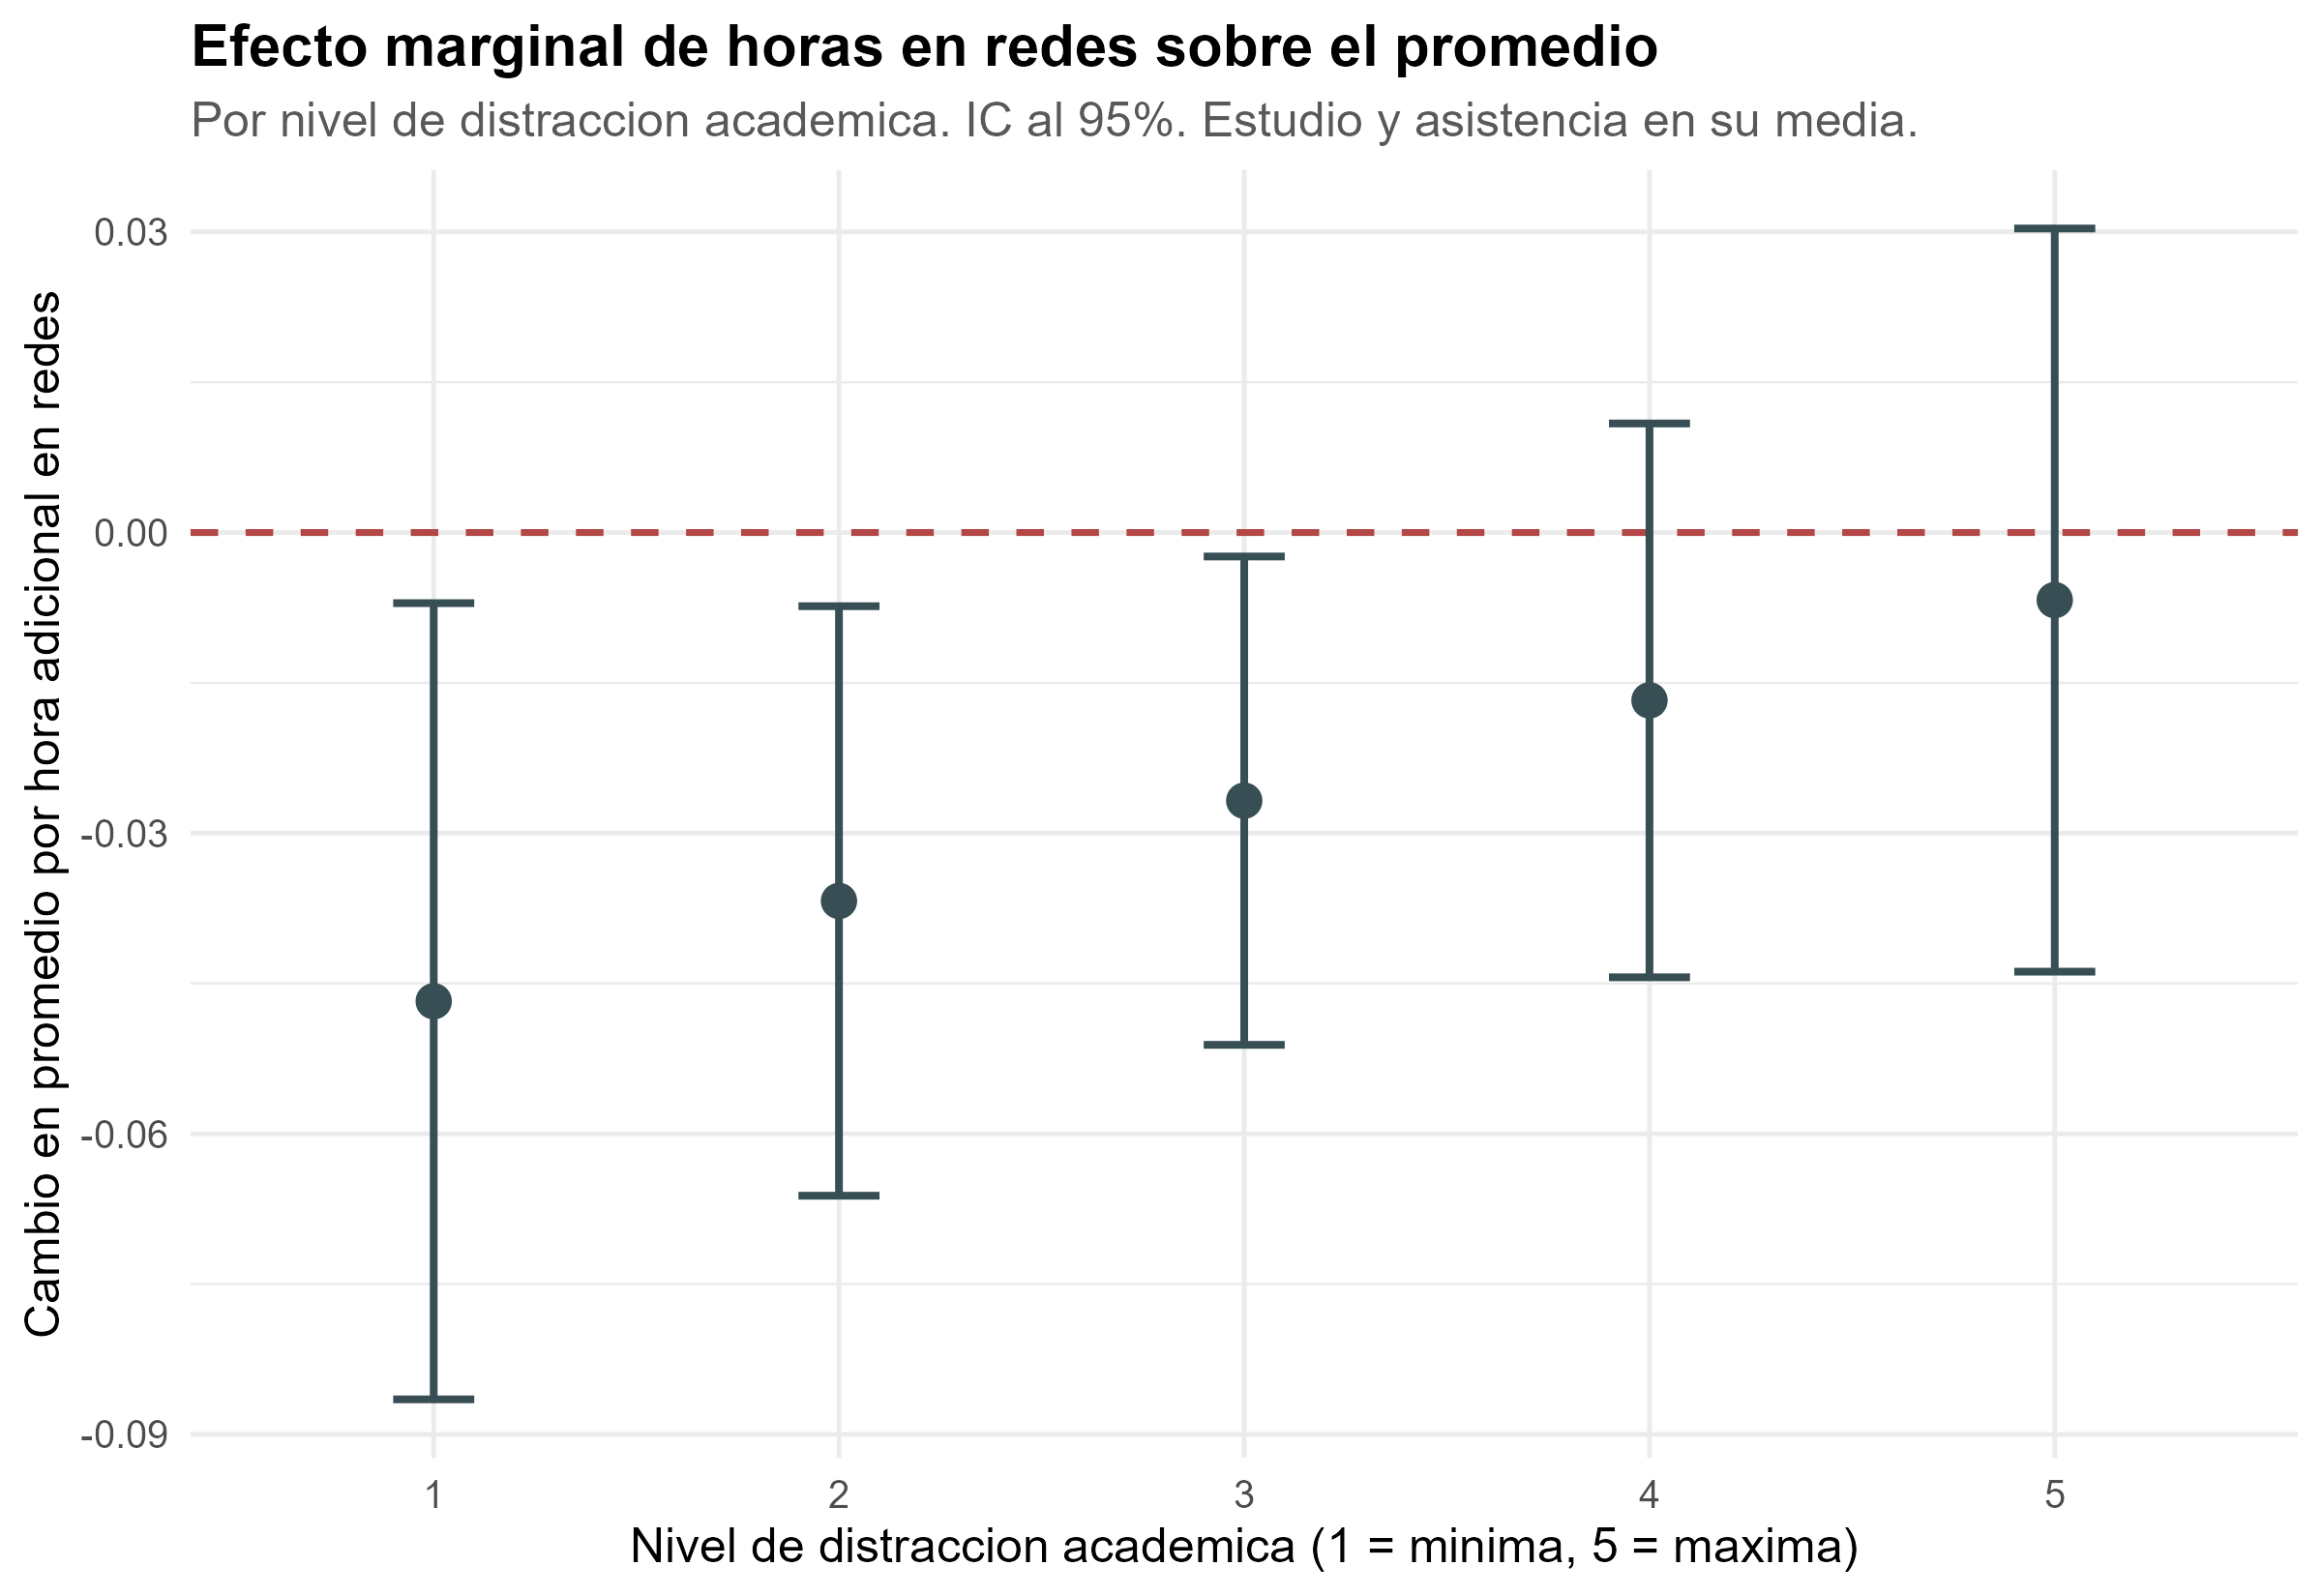
\includegraphics[width=0.7\textwidth]{figuras/figura_07_efecto_marginal_horas_redes.png}
    \caption{Efecto marginal de horas en redes sobre el promedio con intervalos de confianza al 95\%, según nivel de distracción.}
    \label{fig:efecto_marginal}
\end{figure}

La tabla y la Figura~\ref{fig:efecto_marginal} muestran un patrón claro: el efecto negativo de las redes sobre el promedio es estadísticamente significativo para estudiantes con distracción baja o media (niveles 1, 2 y 3), pero deja de serlo para quienes reportan distracción alta (niveles 4 y 5). En estos últimos, el intervalo de confianza cruza el cero, lo que indica que el efecto es incierto en esa subpoblación.

Un estudiante con distracción mínima (nivel 1) que pasa una hora adicional diaria en redes tiene un promedio predicho 0.047 puntos menor, con un rango de \(-0.086\) a \(-0.007\). Para un estudiante con distracción máxima (nivel 5), ese mismo cambio se asocia con apenas \(-0.007\) puntos y el intervalo es tan amplio (\([-0.044, +0.030]\)) que no permite descartar que el efecto sea nulo o incluso positivo. Esto no significa que las redes sean inofensivas para los más distraídos, sino que la muestra no tiene suficiente potencia para detectar el efecto en ese subgrupo.

\begin{table}[H]
\centering
\caption{Intervalos de confianza para predictores fijos del Modelo 3.}
\begin{tabular}{lcc}
\toprule
Predictor & \(\hat\beta\) & IC 95\% \\
\midrule
Horas de estudio & \(+0.069\) & \([+0.037, +0.100]\) \\
Asistencia & \(+0.011\) & \([+0.007, +0.015]\) \\
\bottomrule
\end{tabular}
\label{tab:ic_predictores_fijos}
\end{table}

\subsubsection{Cuadros, gráficos y algoritmos de respaldo}

Los resultados se respaldan con los siguientes elementos producidos por el script:

\begin{itemize}
    \item \textbf{Tablas de coeficientes} con estimaciones, errores estándar, estadísticos \(t\), \(p\)-valores e IC 95\% para los tres modelos (\texttt{13\_}, \texttt{14\_}, \texttt{15\_coeficientes\_*.csv}).
    \item \textbf{Tabla comparativa de modelos} con \(R^2\), \(\sigma\), AIC, BIC y prueba \(F\) secuencial (\texttt{12\_comparacion\_modelos.csv}, \texttt{16\_resumen\_modelos.txt}).
    \item \textbf{Tabla de efectos marginales con IC} por nivel de distracción (\texttt{23\_ic\_efecto\_marginal\_horas\_redes.csv}).
    \item \textbf{Figura 1 - Horas en redes vs. promedio académico (LOESS).} 
    \begin{figure}[H]
        \centering
        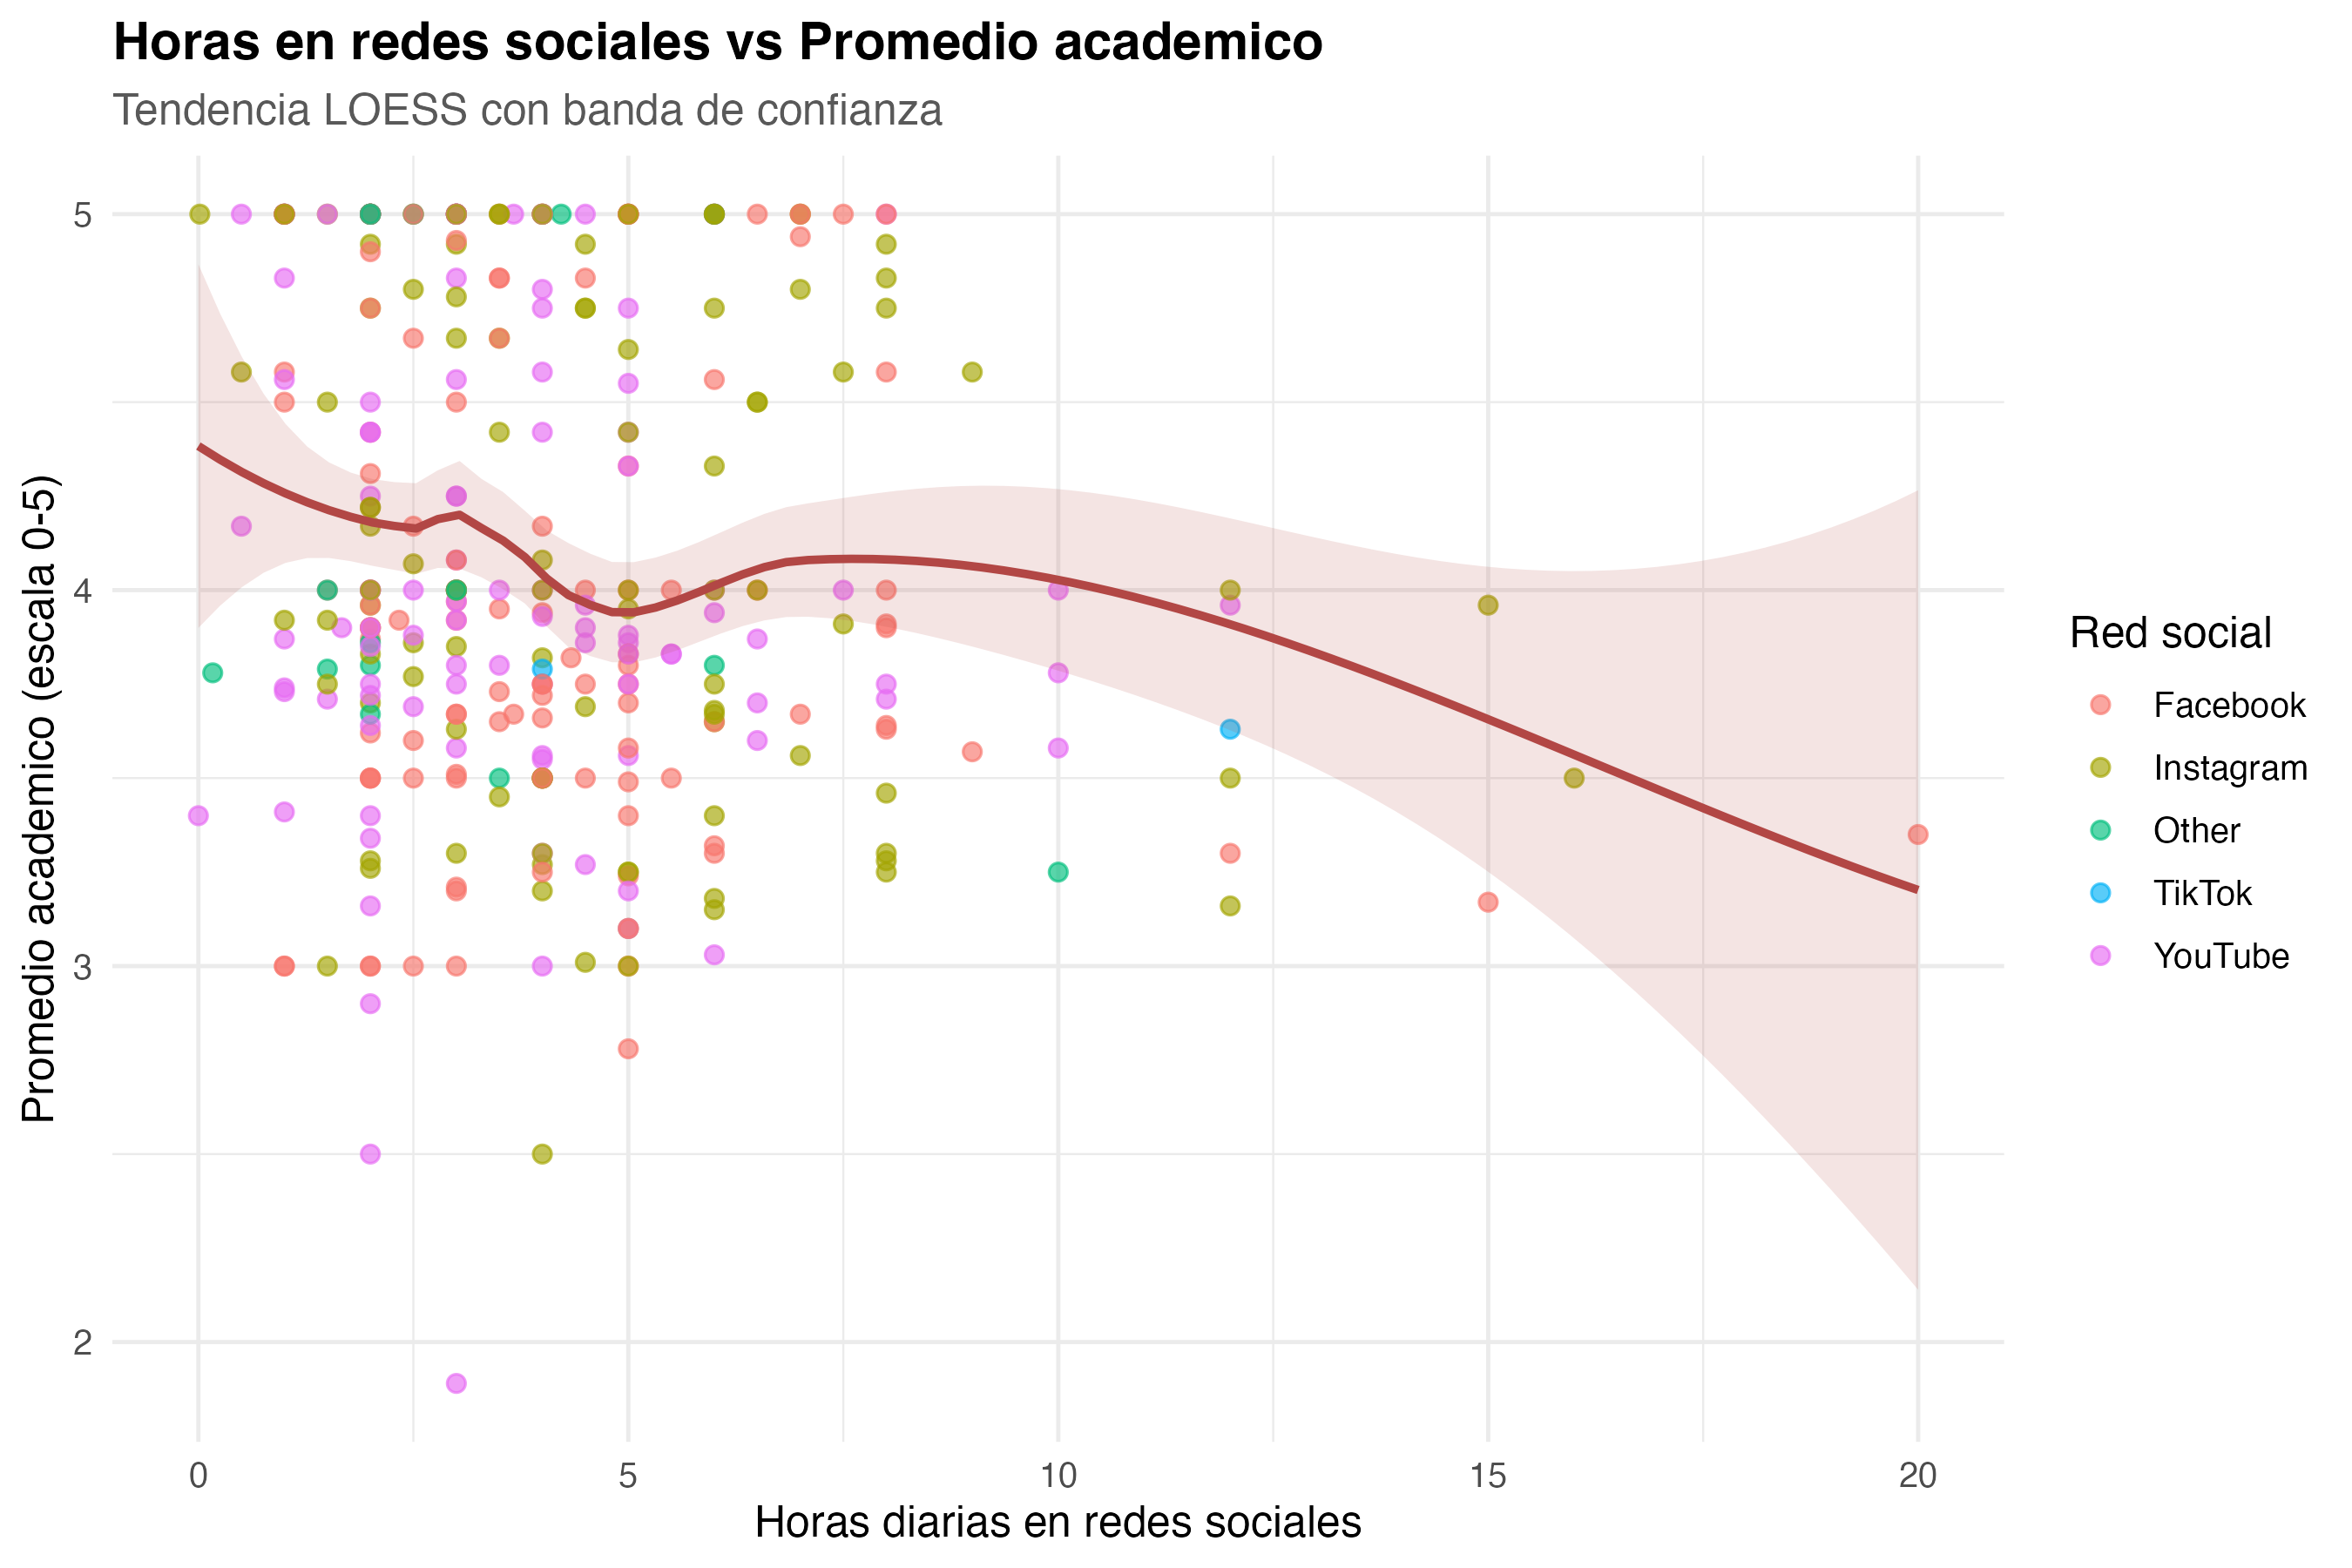
\includegraphics[width=0.7\linewidth]{figuras/figura_01_horas_redes_vs_promedio.png}
    \end{figure}
    
    La curva de tendencia muestra que el promedio se mantiene relativamente estable (alrededor de 4.0–4.3) hasta aproximadamente 6 horas diarias, a partir de donde desciende de forma marcada. La alta variabilidad en la franja 0–5 horas es coherente con la dispersión de colores por plataforma, lo que sugiere que la plataforma por sí sola no explica diferencias importantes.
    \item \textbf{Figura 2 - Boxplot por categoría de uso.}
    \begin{figure}[H]
        \centering
        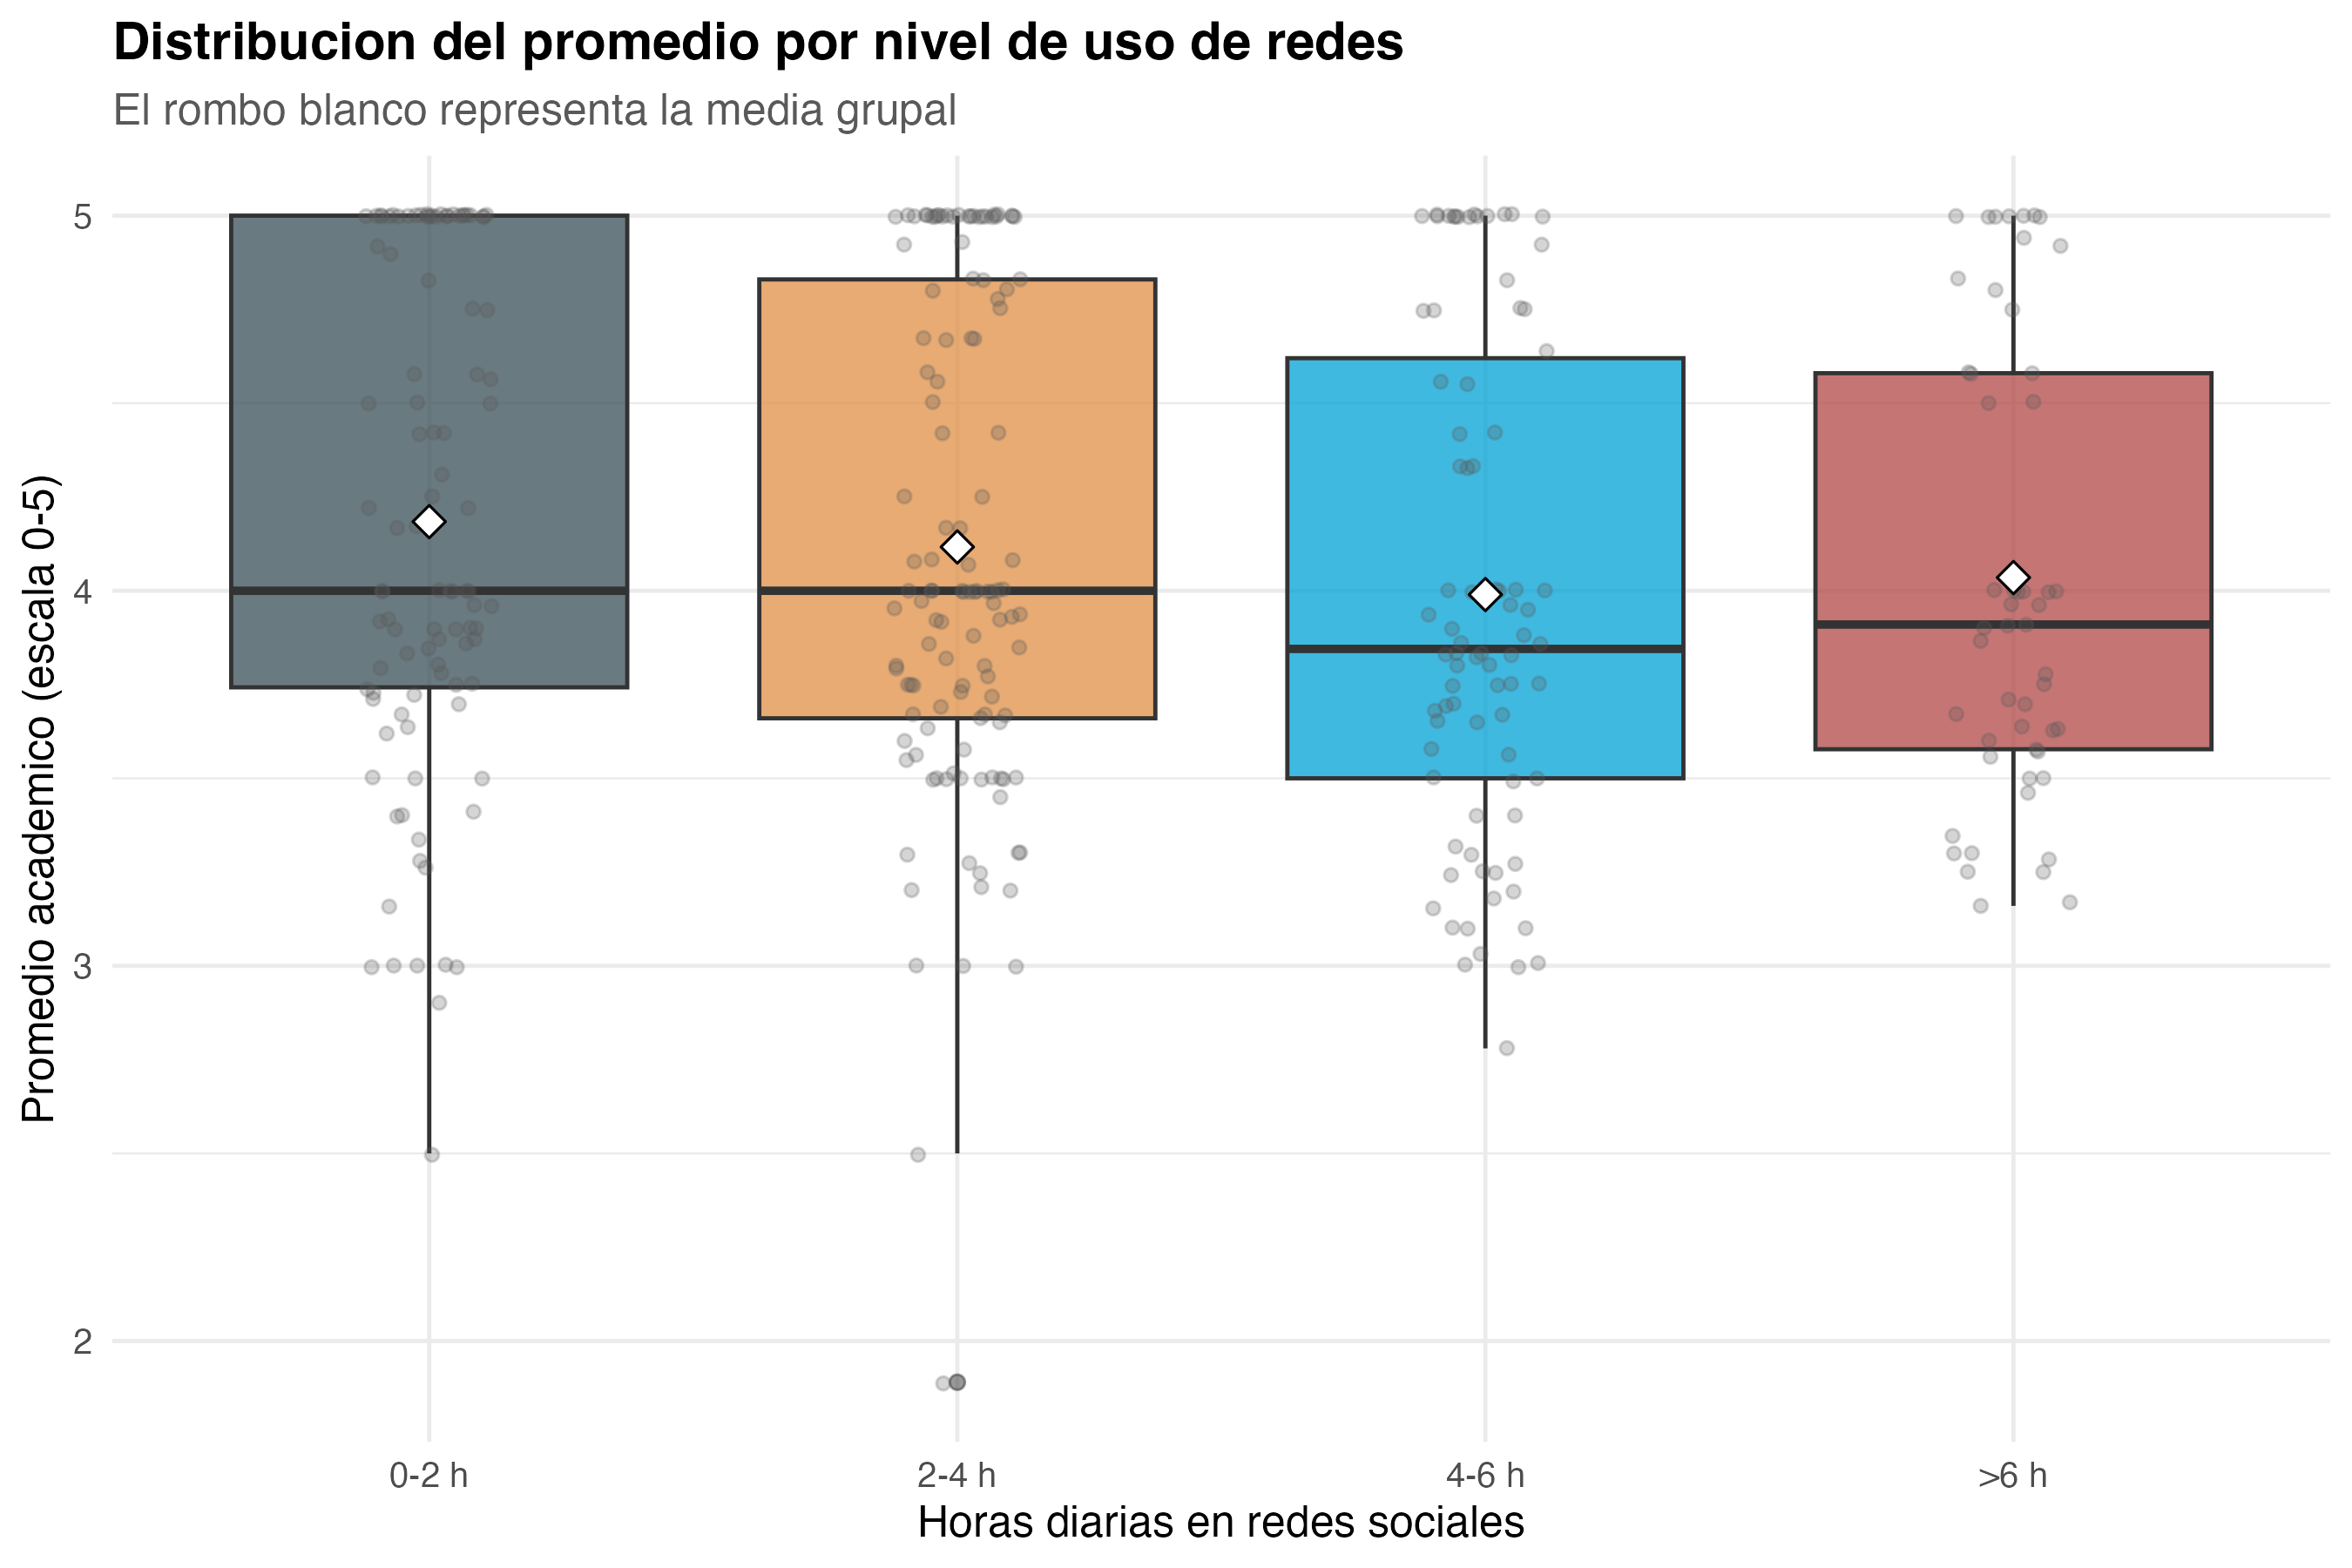
\includegraphics[width=0.7\linewidth]{figuras/figura_02_boxplot_uso_redes.png}
    \end{figure}
    
    Las medianas son similares entre los grupos 0–2 h, 2–4 h y 4–6 h (alrededor de 4.0), mientras que el grupo \(>6\) h muestra una mediana ligeramente inferior (\(\sim3.9\)) y mayor presencia de valores bajos. El descenso no es dramático en términos absolutos pero sí consistente.
    \item \textbf{Figura 3 - Horas de estudio vs. promedio.}
    \begin{figure}[H]
        \centering
        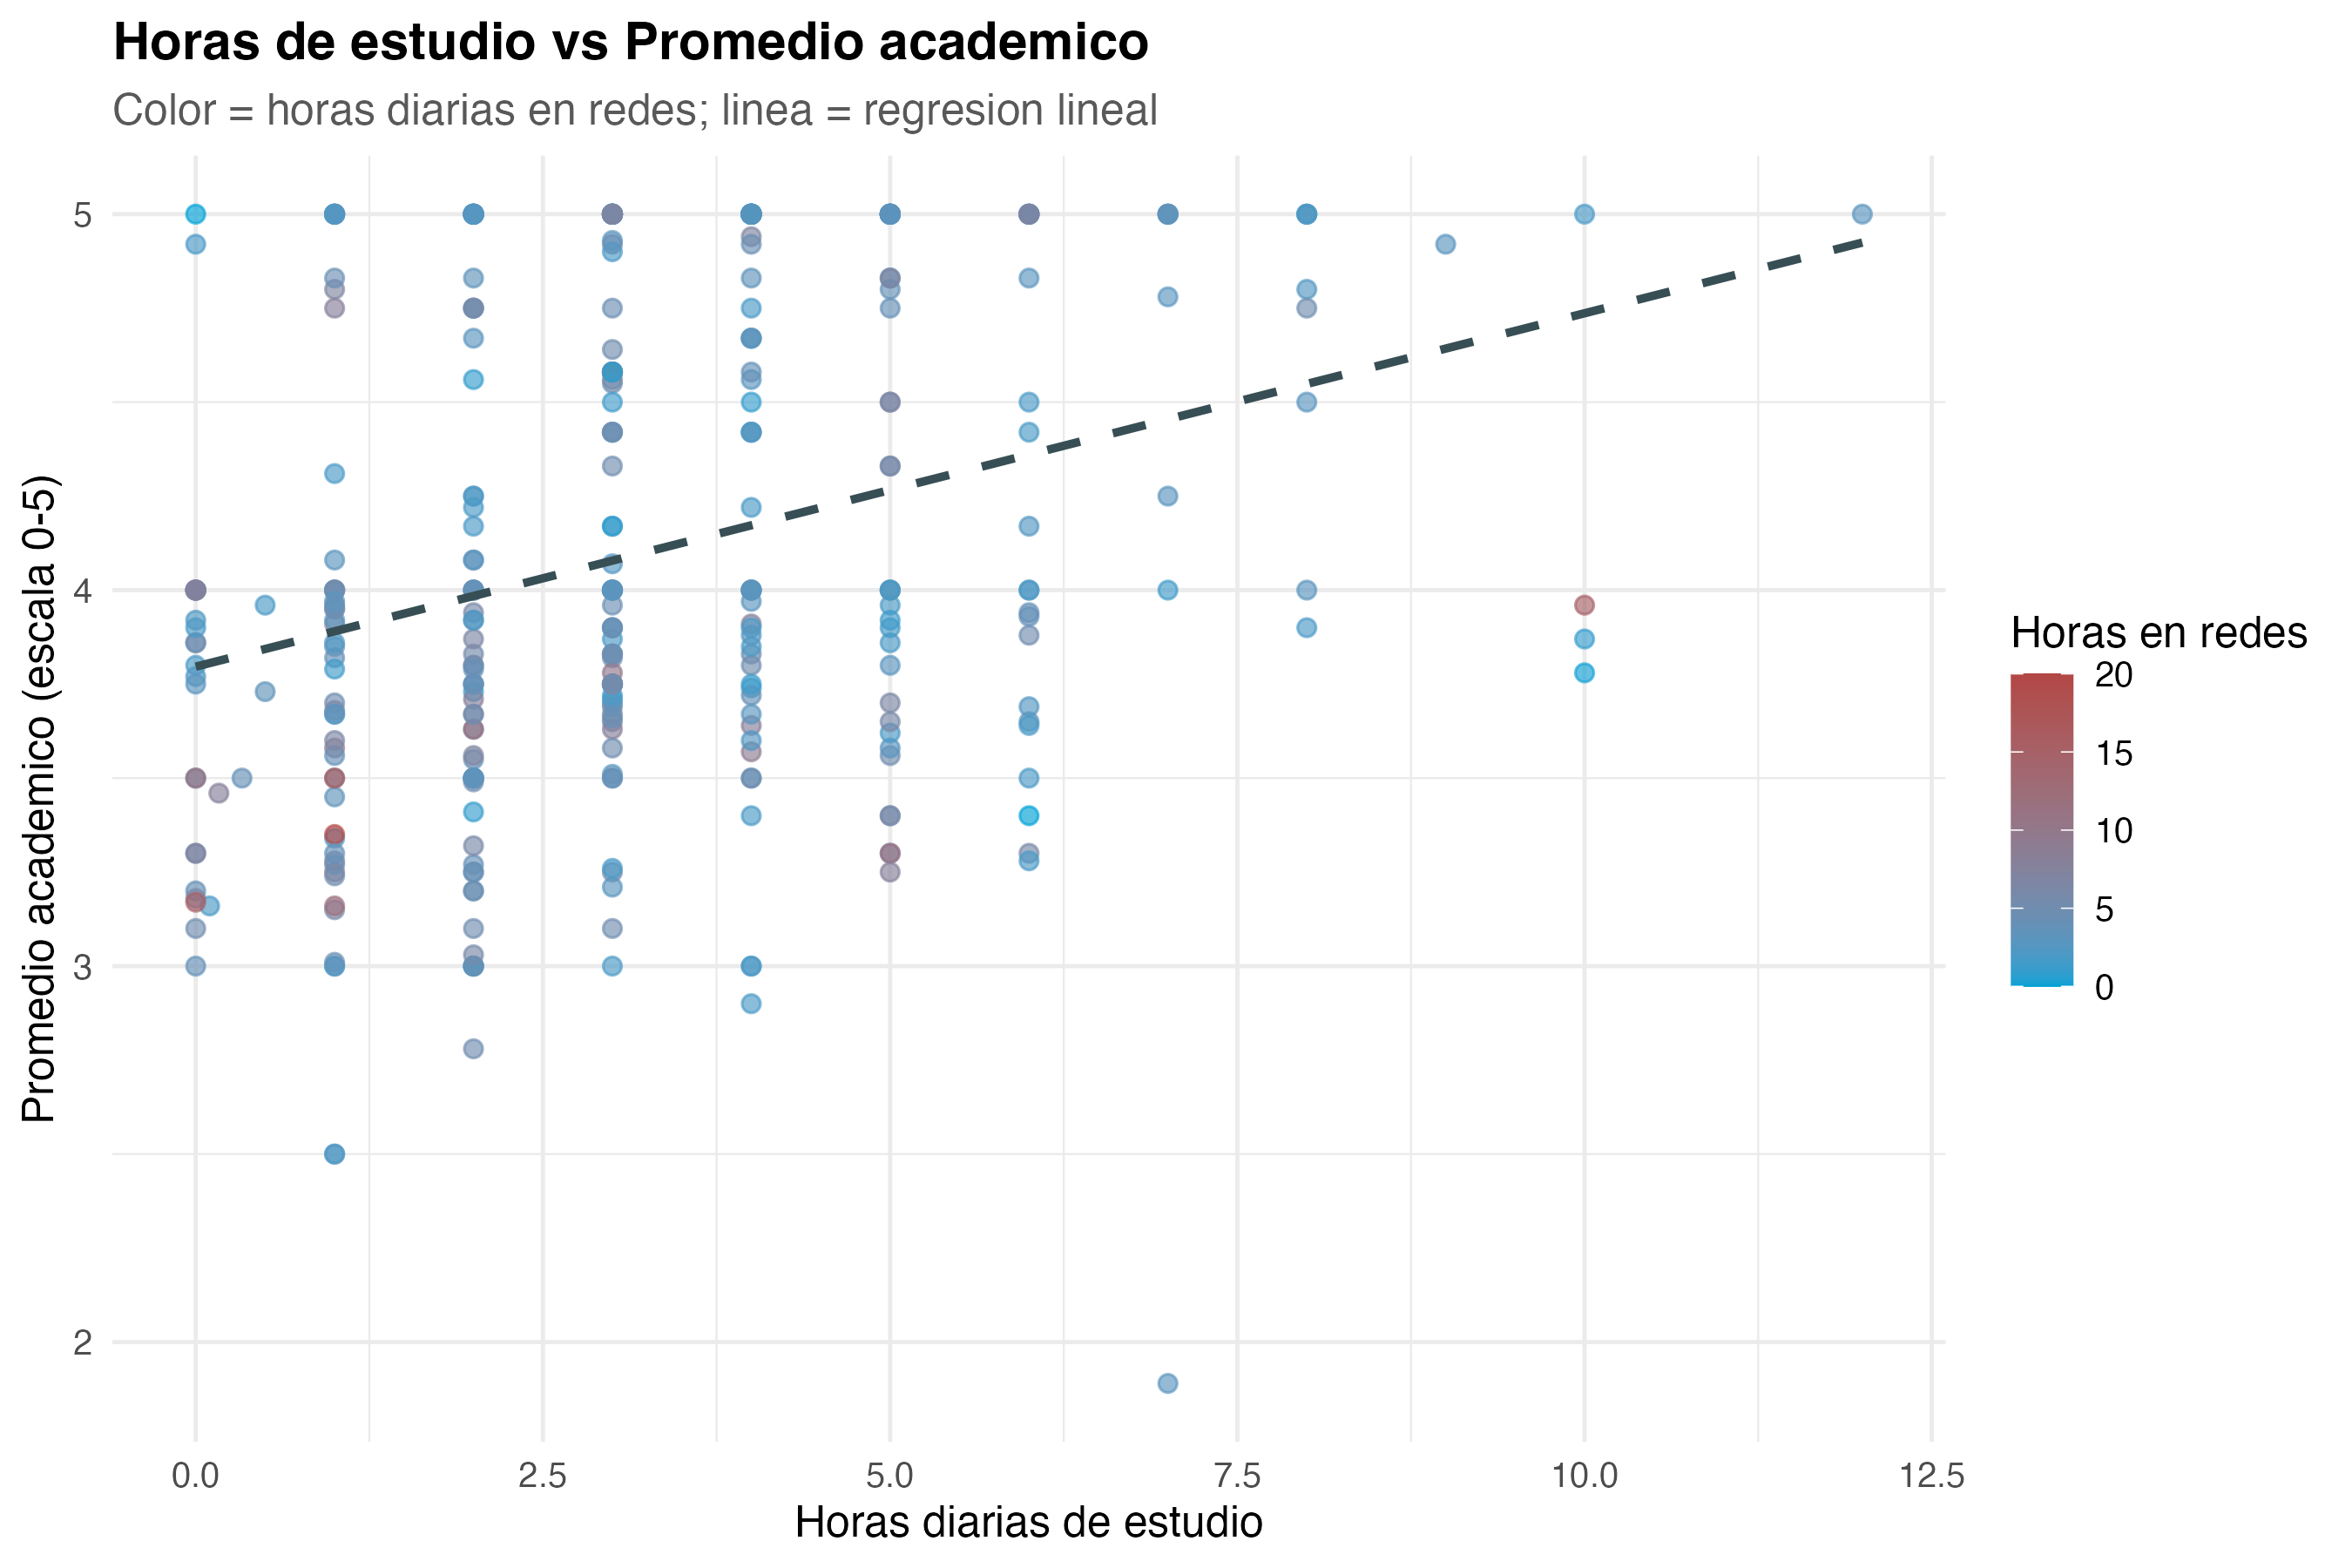
\includegraphics[width=0.7\linewidth]{figuras/figura_03_horas_estudio_vs_promedio.png}
    \end{figure}
    
    La regresión lineal muestra una pendiente positiva clara: más horas de estudio se asocian a mayor promedio. Los puntos de color más rojo (muchas horas en redes) no se concentran consistentemente en la parte baja del gráfico, lo que anticipa que el efecto de las redes puede ser moderado por otras variables.
    \item \textbf{Figura 4 - Promedio por plataforma.}
    \begin{figure}[H]
        \centering
        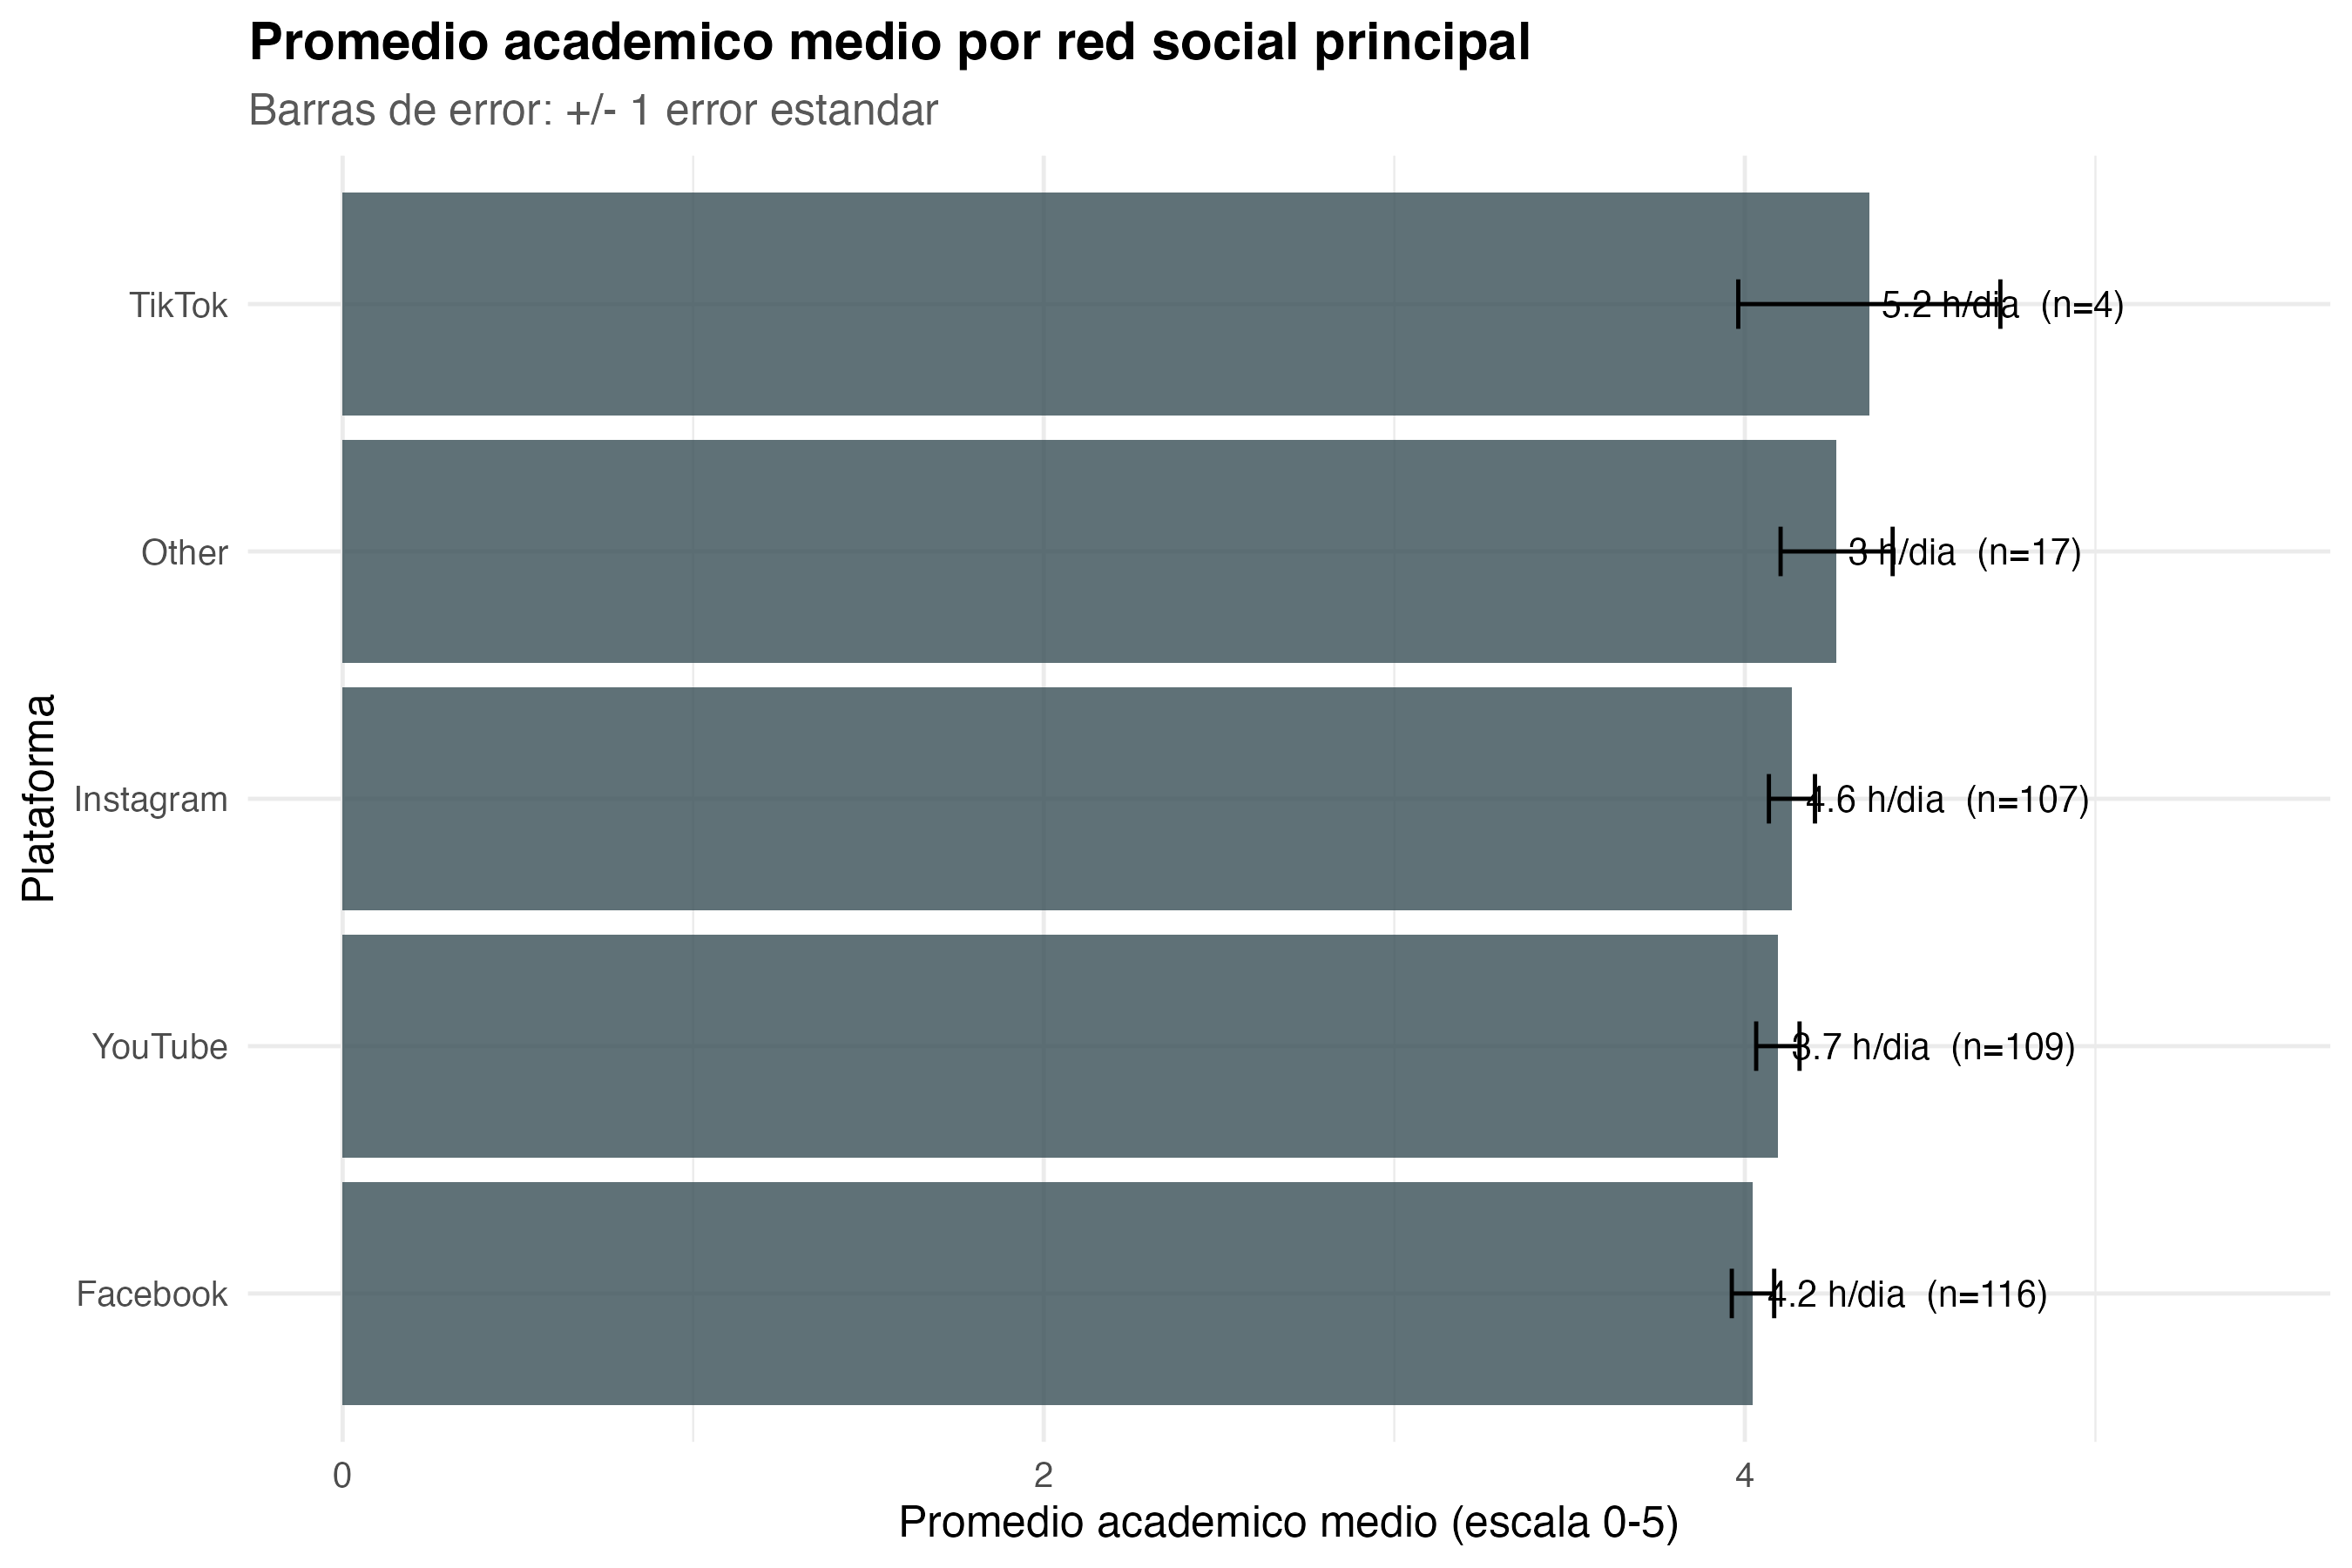
\includegraphics[width=0.7\linewidth]{figuras/figura_04_promedio_por_plataforma.png}
    \end{figure}
    
    Las diferencias entre plataformas son pequeñas (rango \(\approx 4.0\)–\(4.3\)). TikTok aparece con el promedio más alto pero con \(n=4\), lo que hace que esta estimación sea muy inestable. Facebook y YouTube concentran la mayoría de observaciones.
    \item \textbf{Figura 5 - Heatmap de uso de redes \(\times\) distracción.}
    \begin{figure}[H]
        \centering
        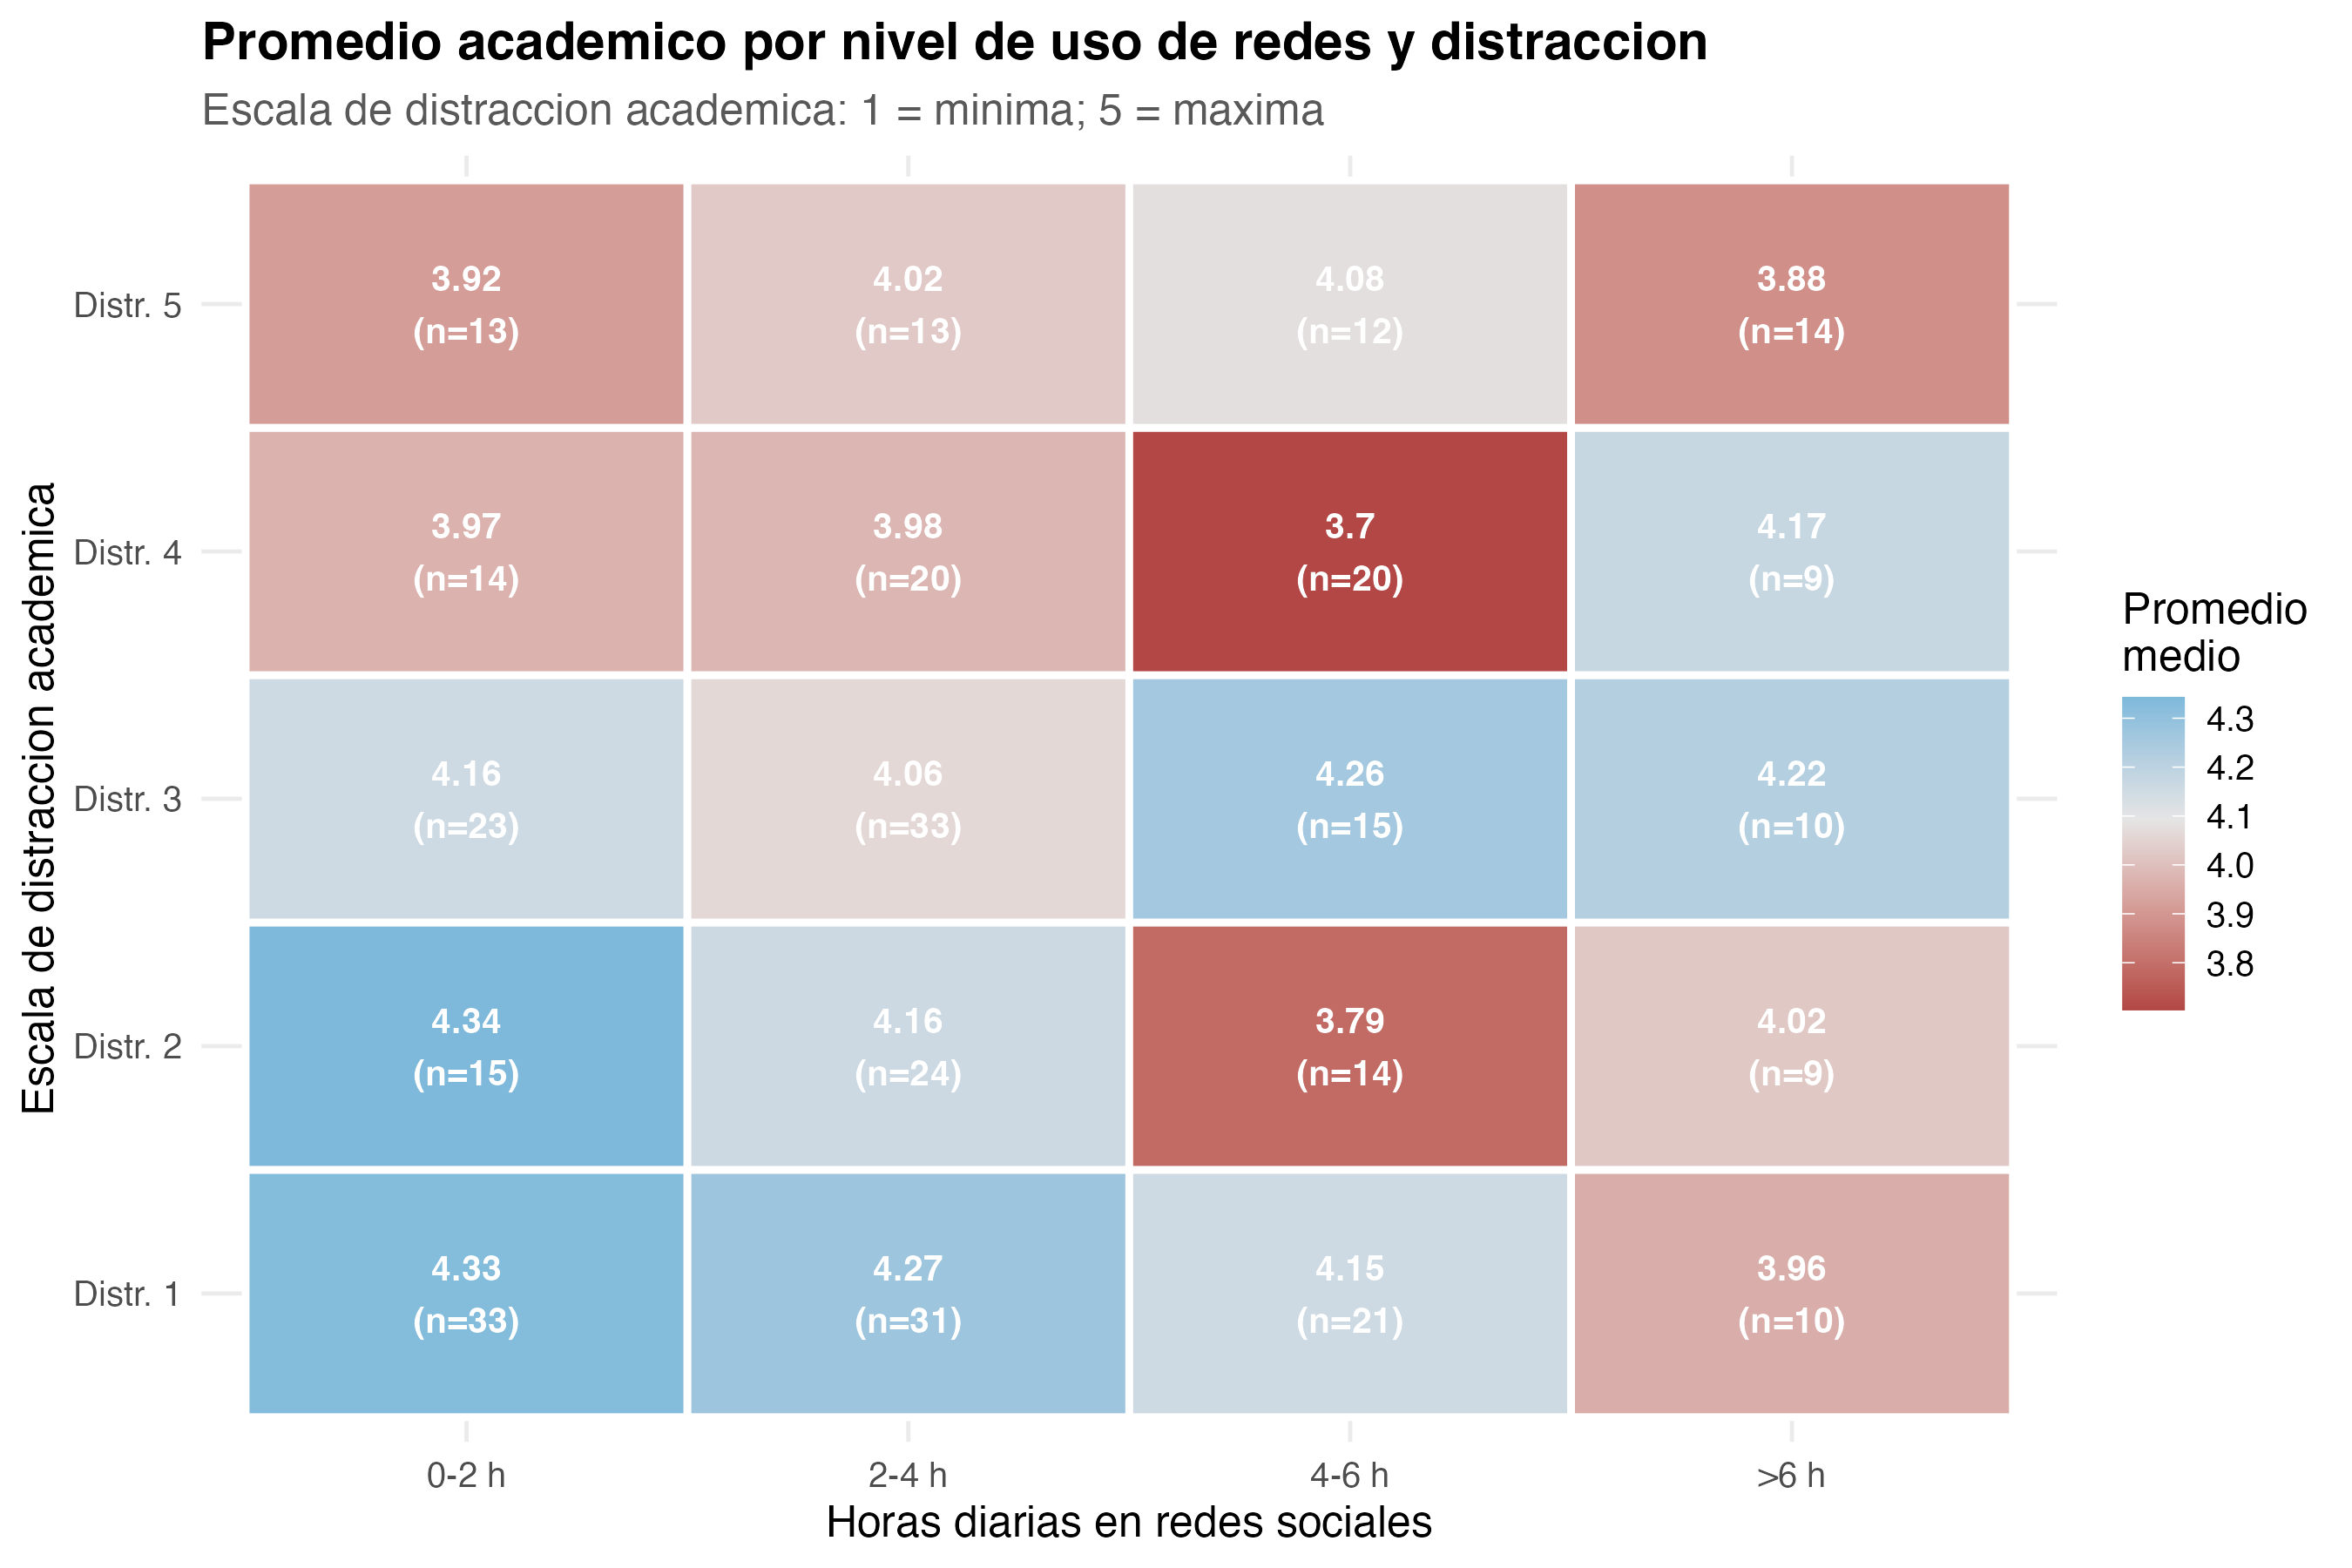
\includegraphics[width=0.7\linewidth]{figuras/figura_05_heatmap_redes_distraccion.png}
    \end{figure}
    
    El patrón más consistente es que en niveles de distracción baja (Distr. 1 y 2), el promedio decrece conforme aumentan las horas en redes. En niveles altos de distracción (Distr. 4 y 5), el patrón es menos monótono, con algunas celdas de promedio relativamente alto asociadas a uso moderado o alto de redes. Esta heterogeneidad motivó incluir el término de interacción en el modelo.
    \item \textbf{Figura 6 - Predicciones del Modelo 3} 
    \begin{figure}[H]
        \centering
        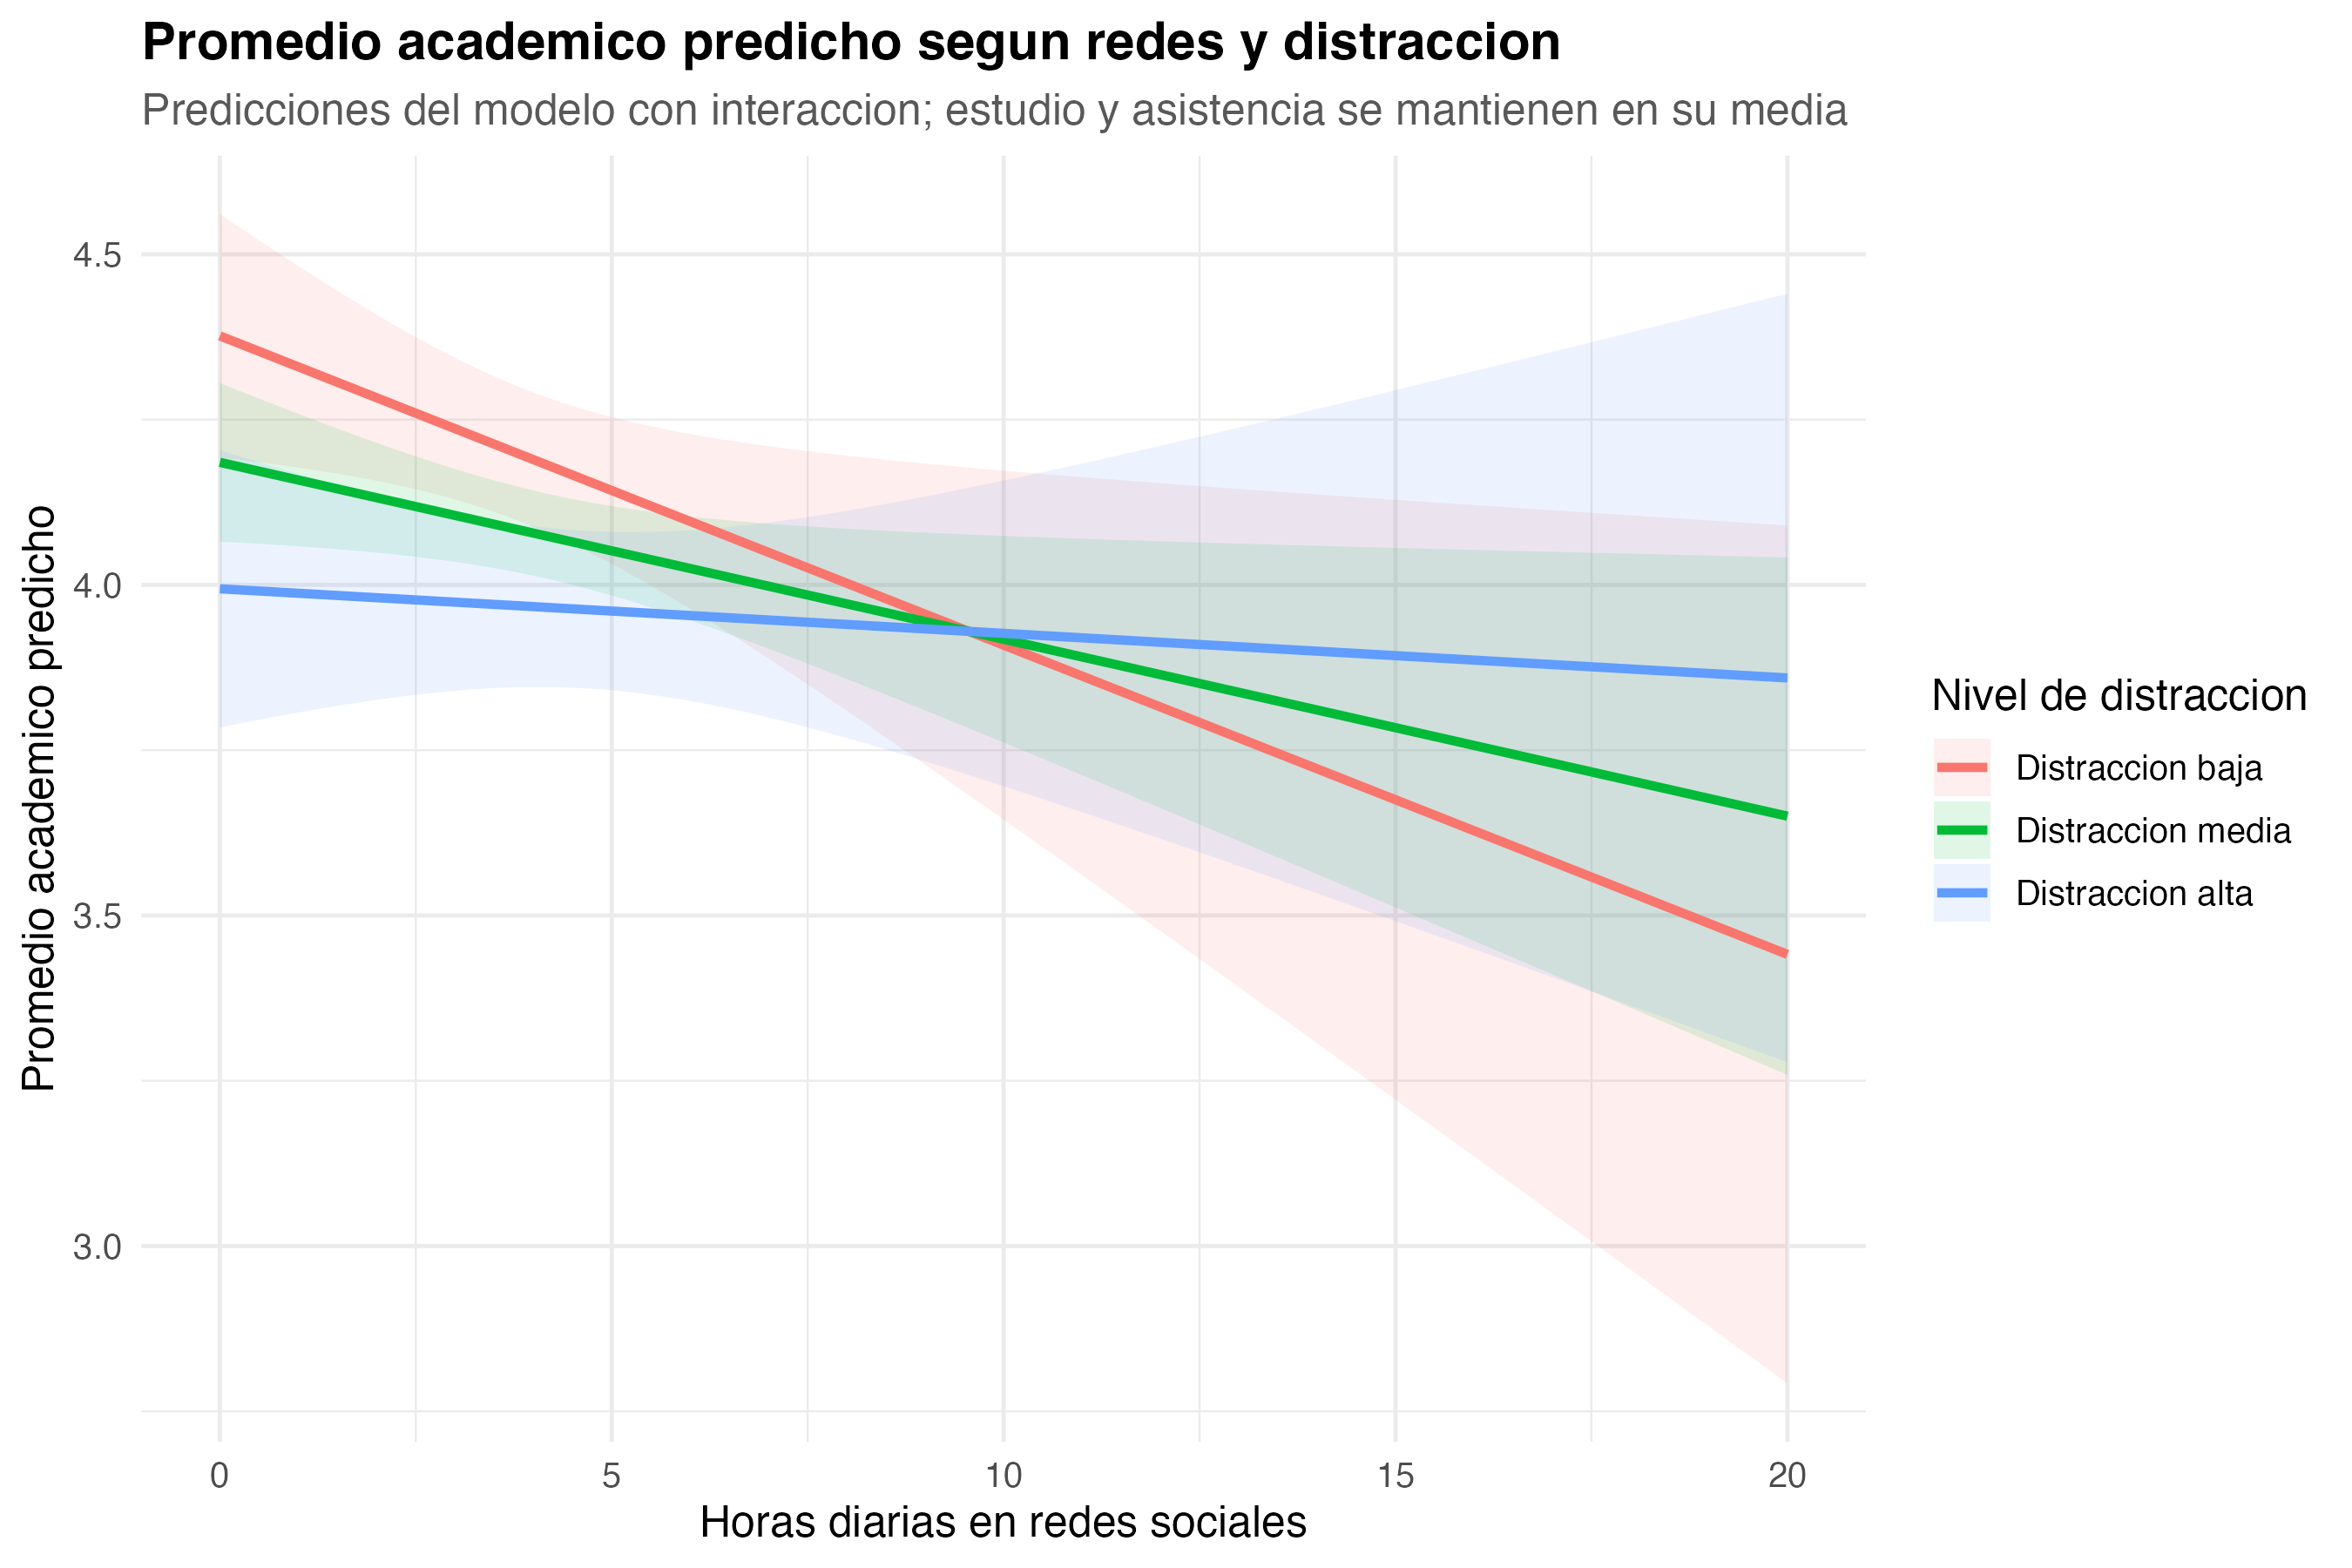
\includegraphics[width=0.7\linewidth]{figuras/figura_06_predicciones_modelo_interaccion.png}
    \end{figure}
    
    Sintetiza el hallazgo principal mostrando pendientes diferenciadas por nivel de distracción.
    \item \textbf{Figura 7 - Efecto marginal con IC}
    \begin{figure}[H]
        \centering
        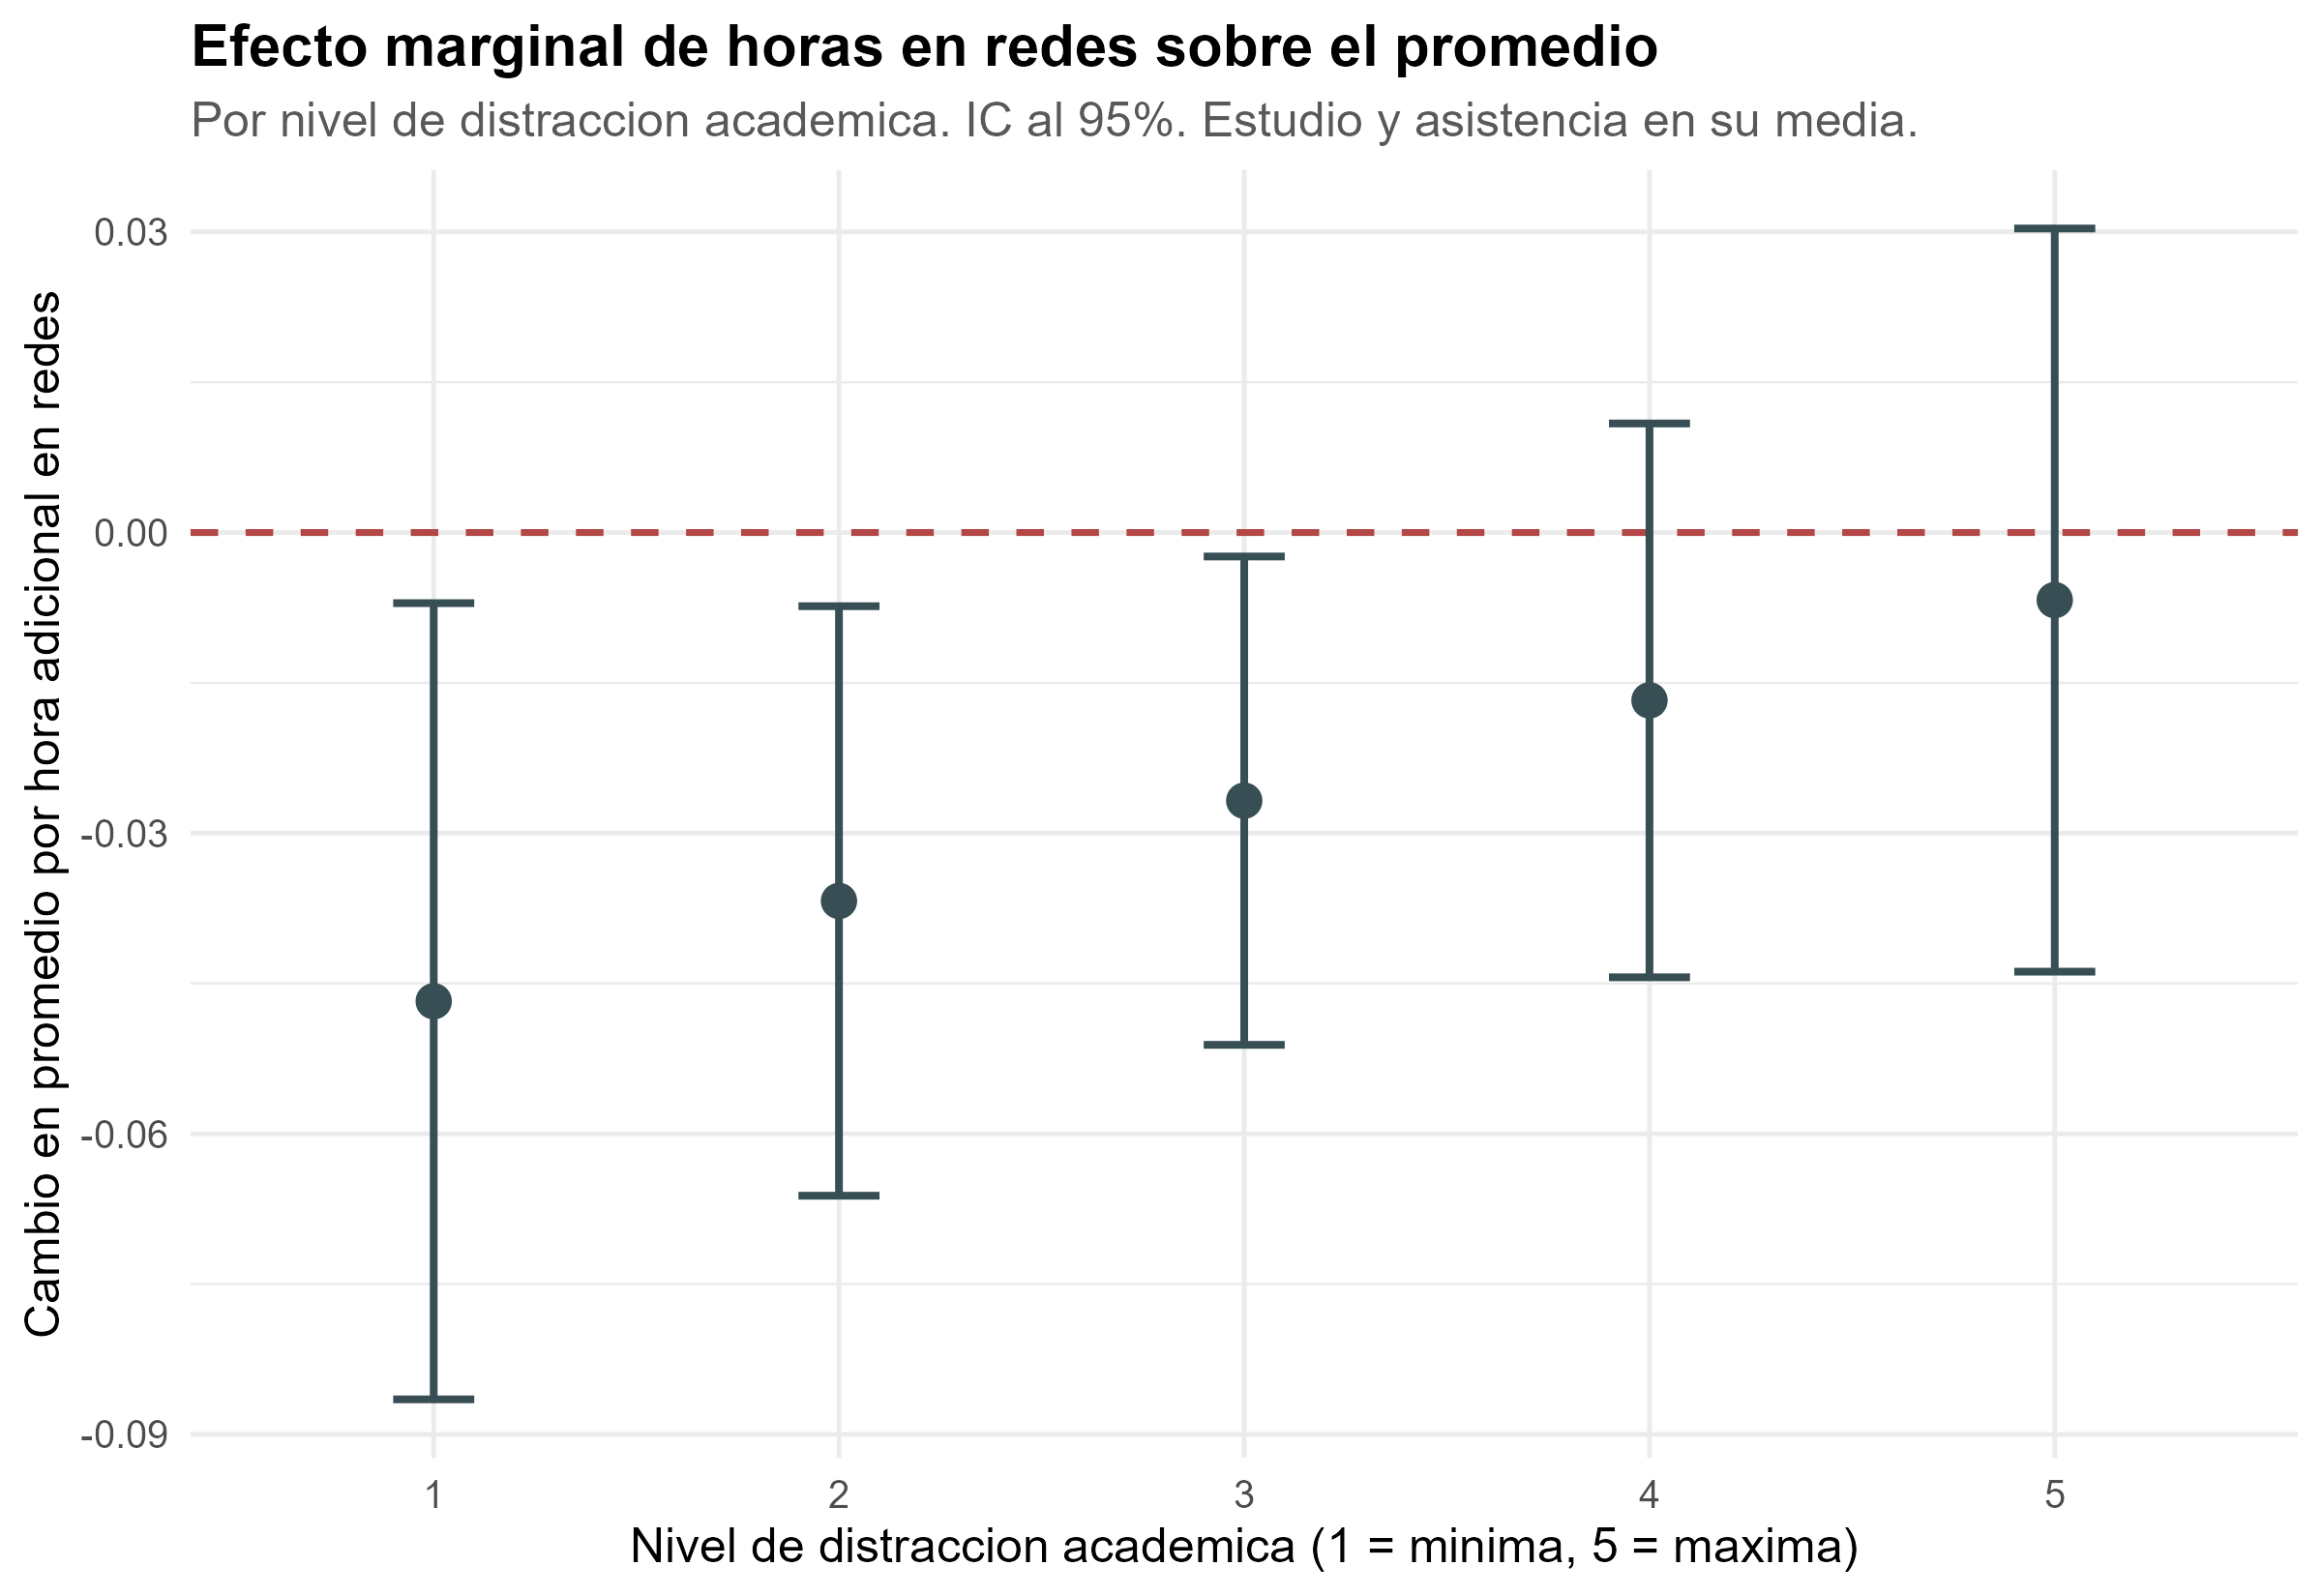
\includegraphics[width=0.7\linewidth]{figuras/figura_07_efecto_marginal_horas_redes.png}
    \end{figure}
    
    Muestra para qué niveles de distracción el efecto de las redes es estadísticamente significativo. Las barras que no cruzan el cero (niveles 1–3) indican efectos detectables; las que sí lo cruzan (niveles 4–5) indican incertidumbre.
    \item \textbf{Diagnósticos 1–4}: residuales vs. ajustados, QQ plot, histograma de residuales y distancia de Cook.

    \begin{figure}[H]
        \centering
        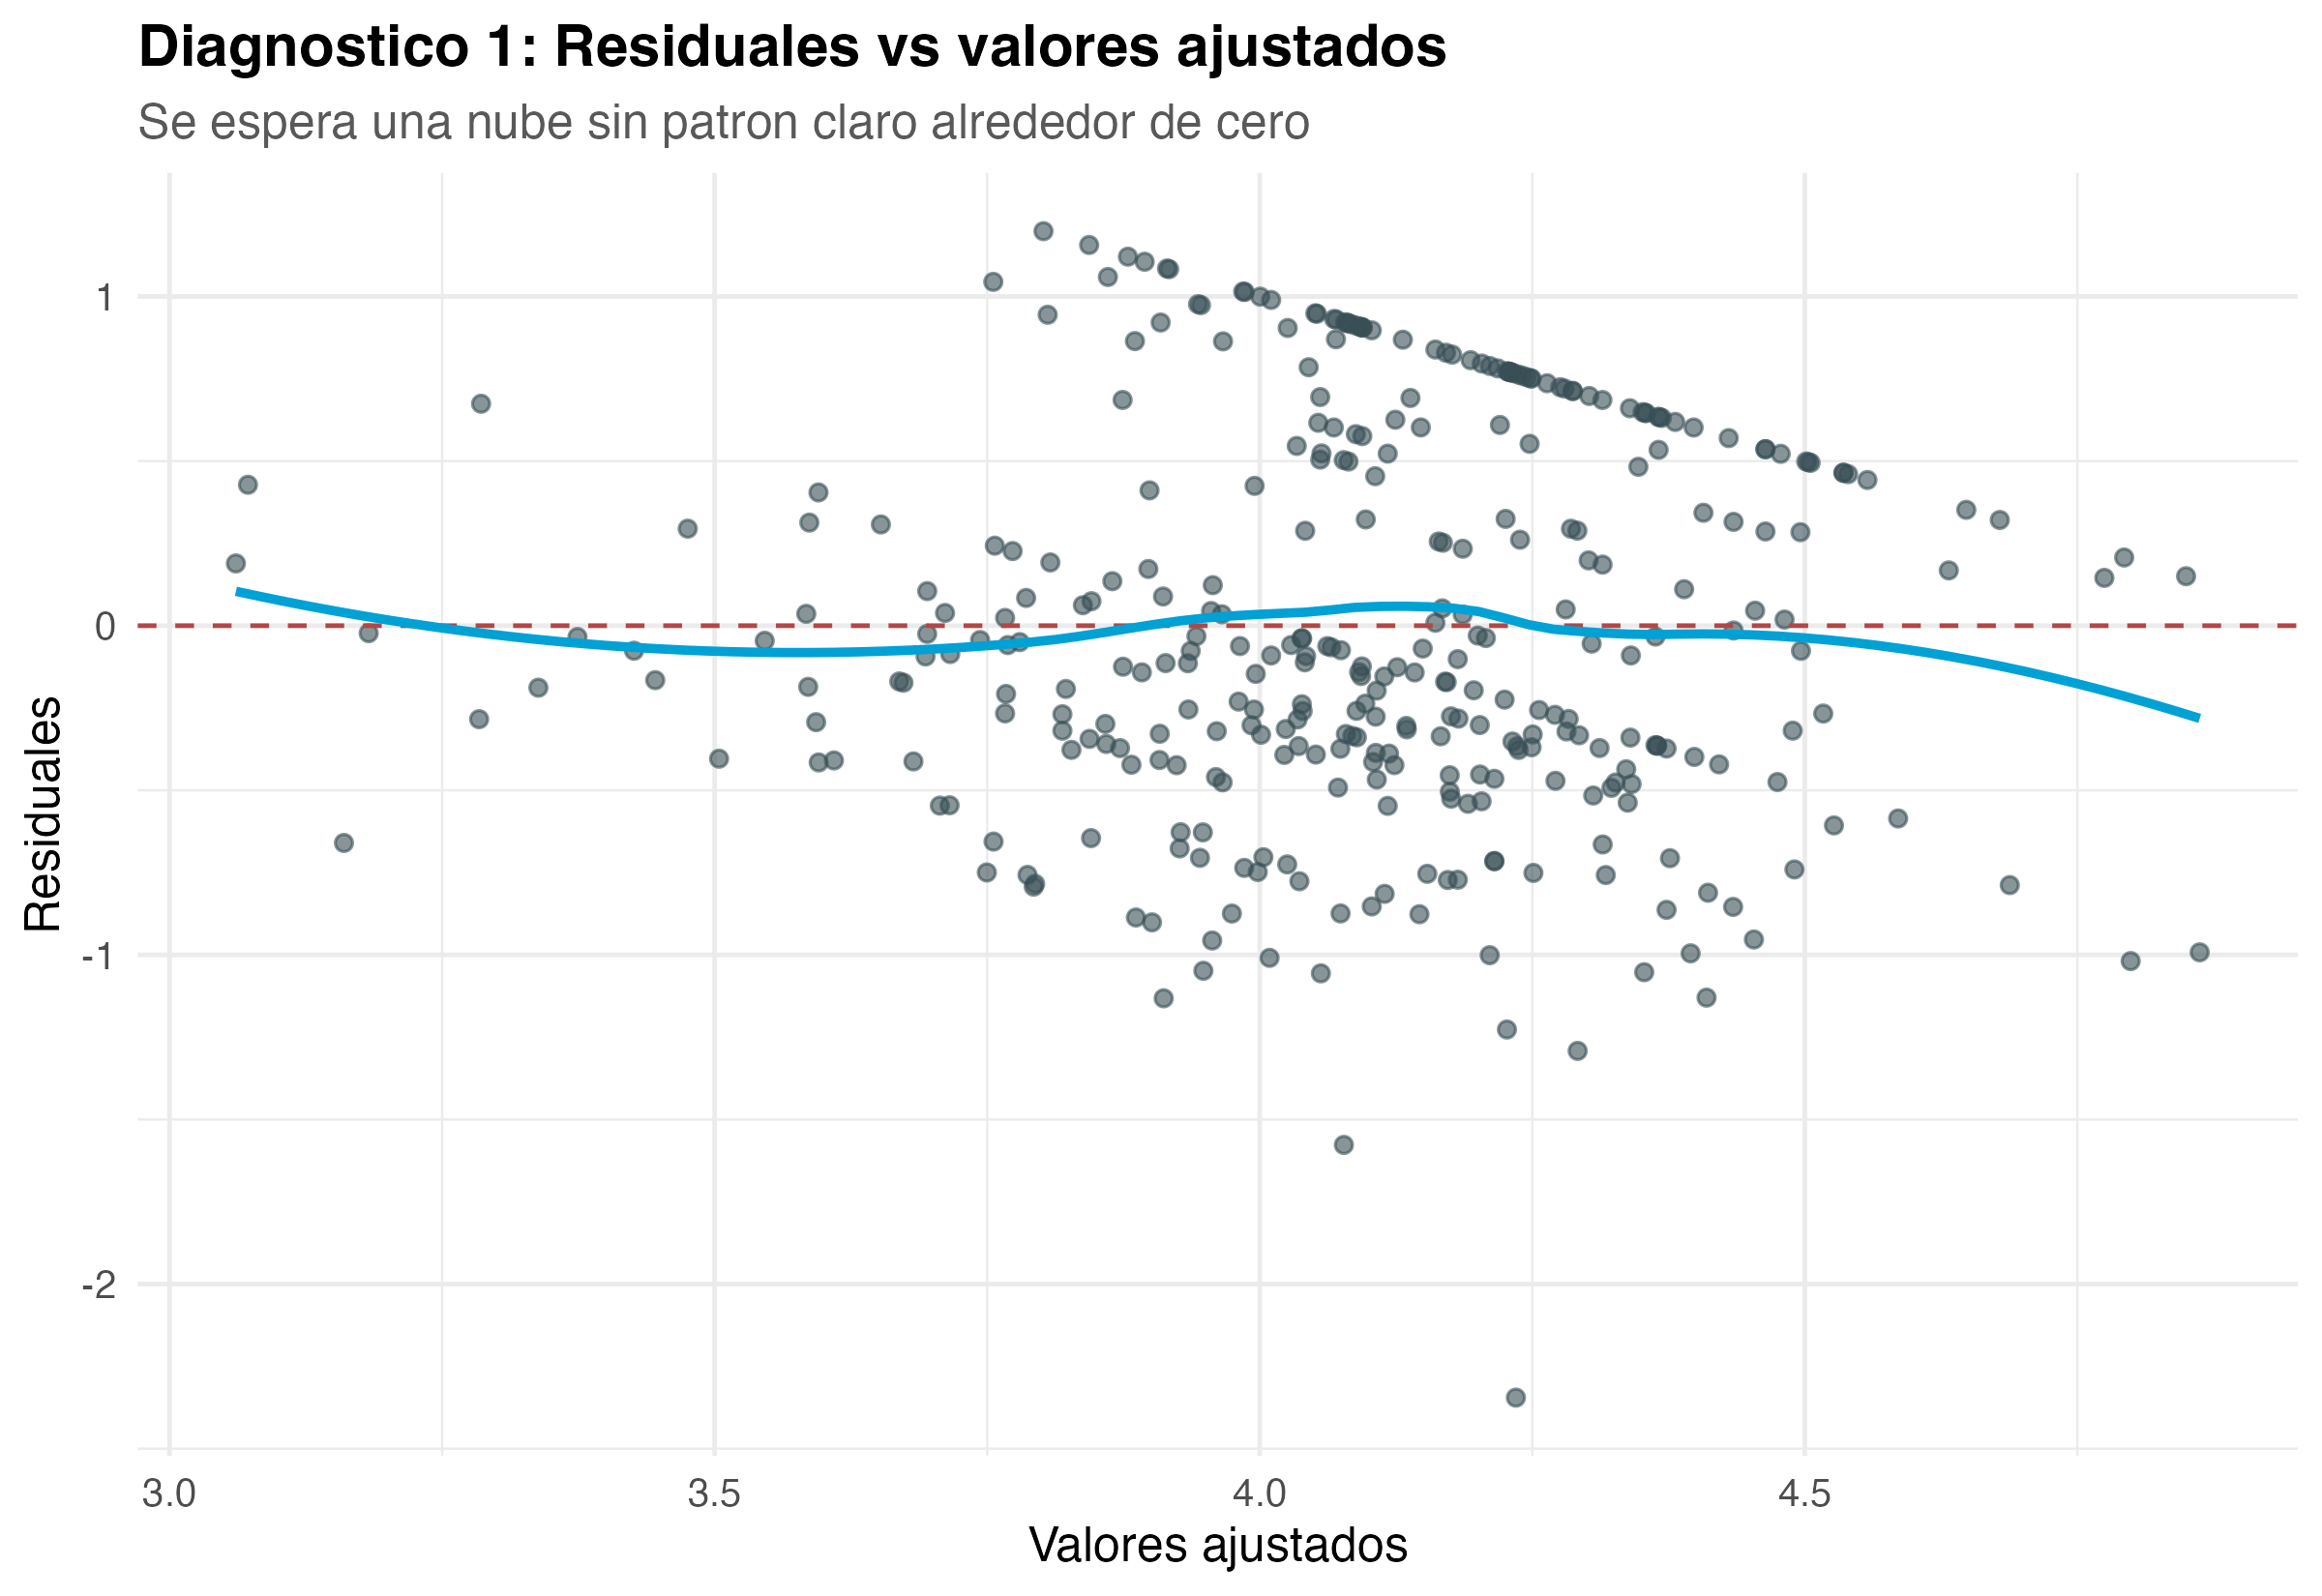
\includegraphics[width=0.7\linewidth]{figuras/diagnostico_01_residuales_vs_ajustados.png}
    \end{figure}
    \begin{figure}[H]
        \centering
        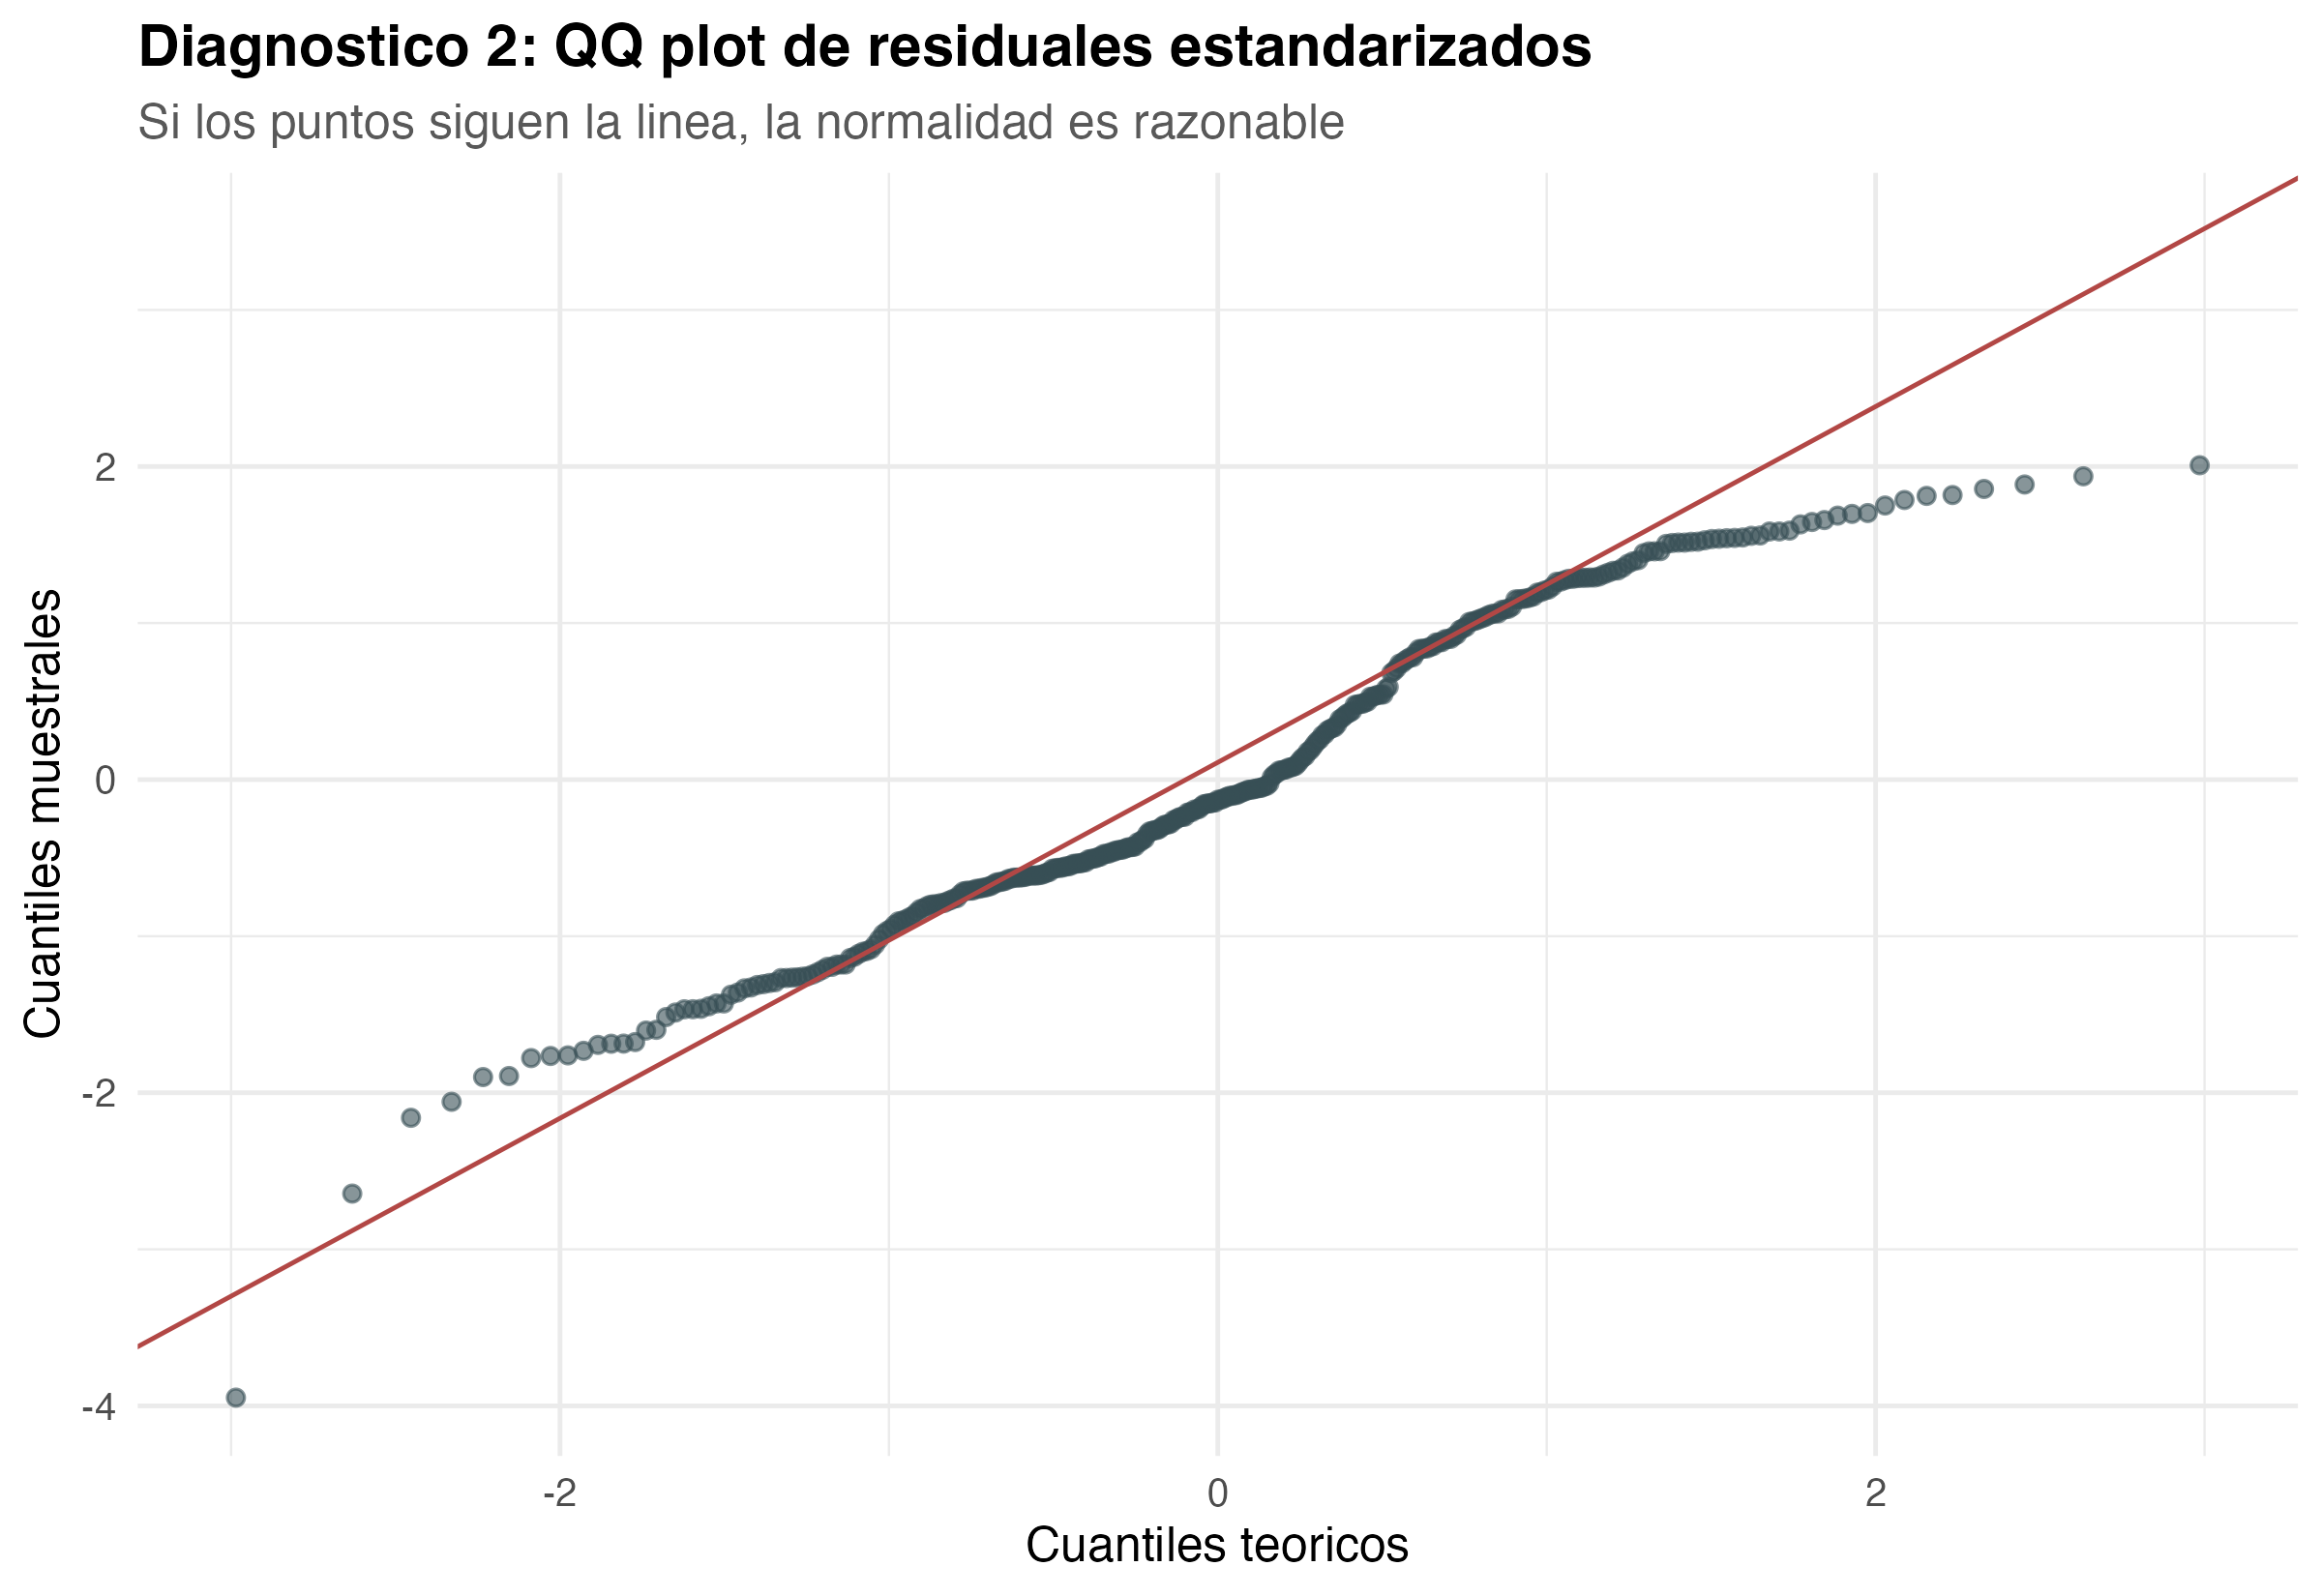
\includegraphics[width=0.7\linewidth]{figuras/diagnostico_02_qqplot_residuales.png}
    \end{figure}
    \begin{figure}[H]
        \centering
        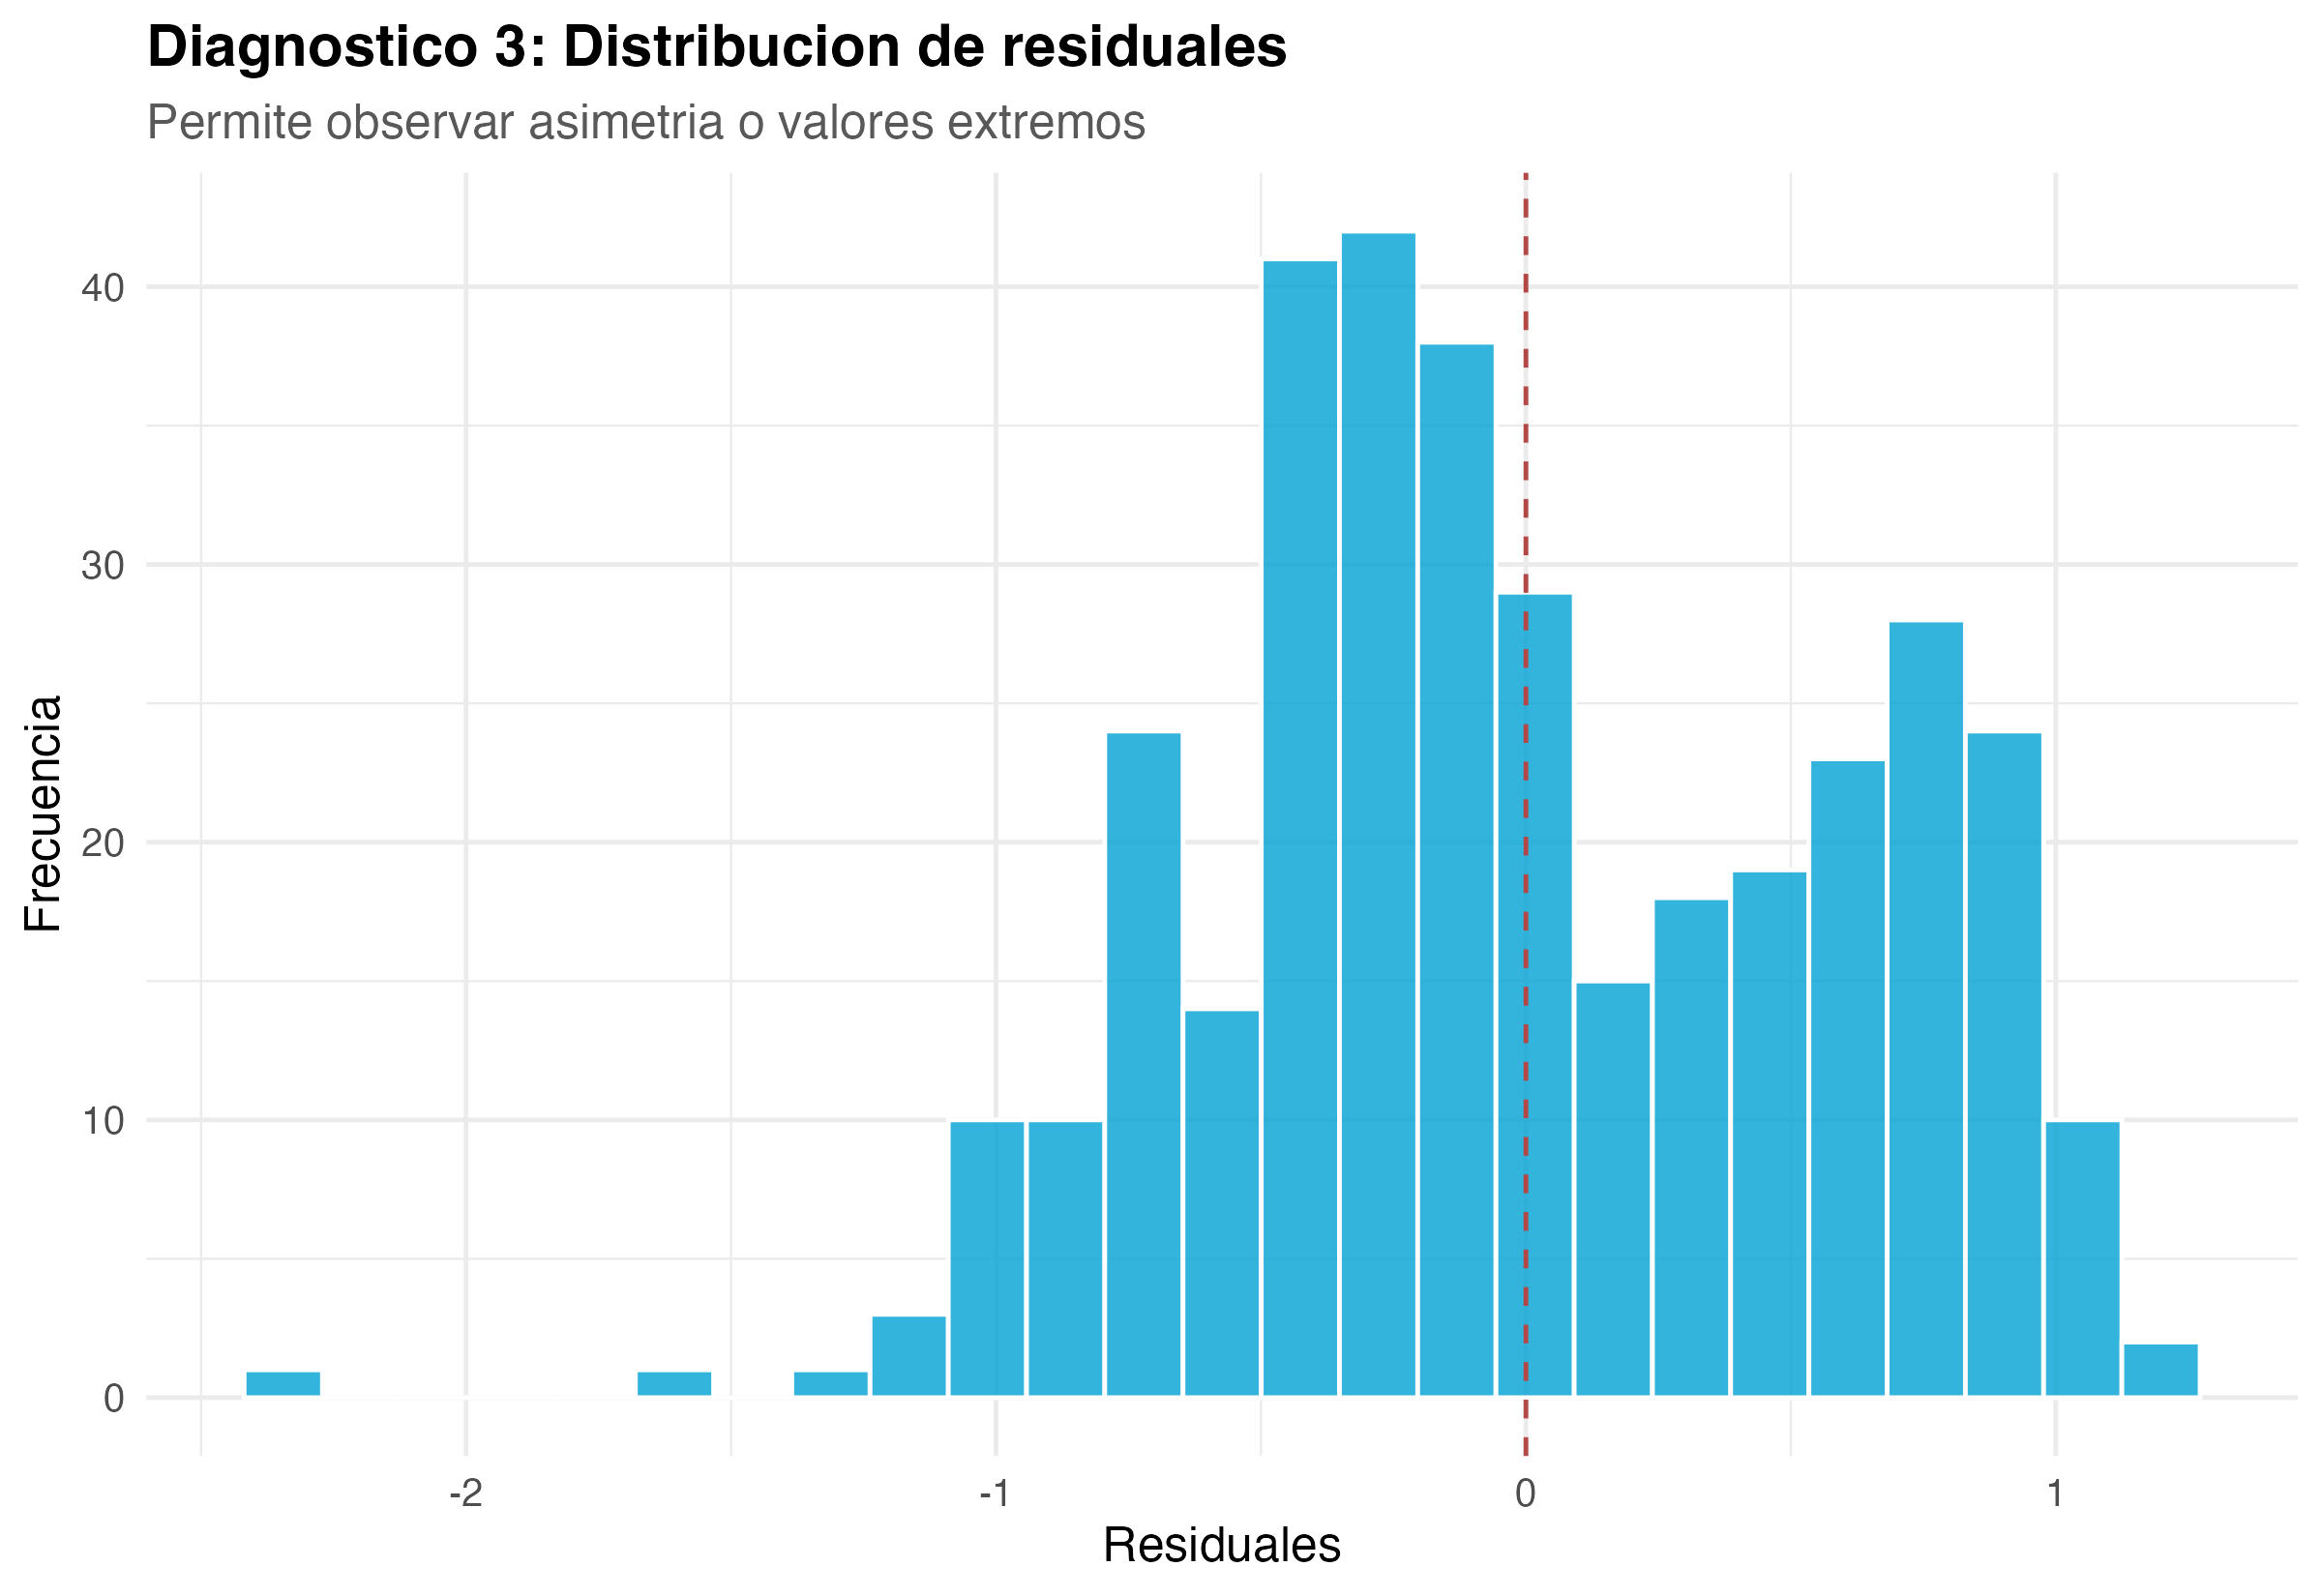
\includegraphics[width=0.7\linewidth]{figuras/diagnostico_03_histograma_residuales.png}
    \end{figure}
    \begin{figure}[H]
        \centering
        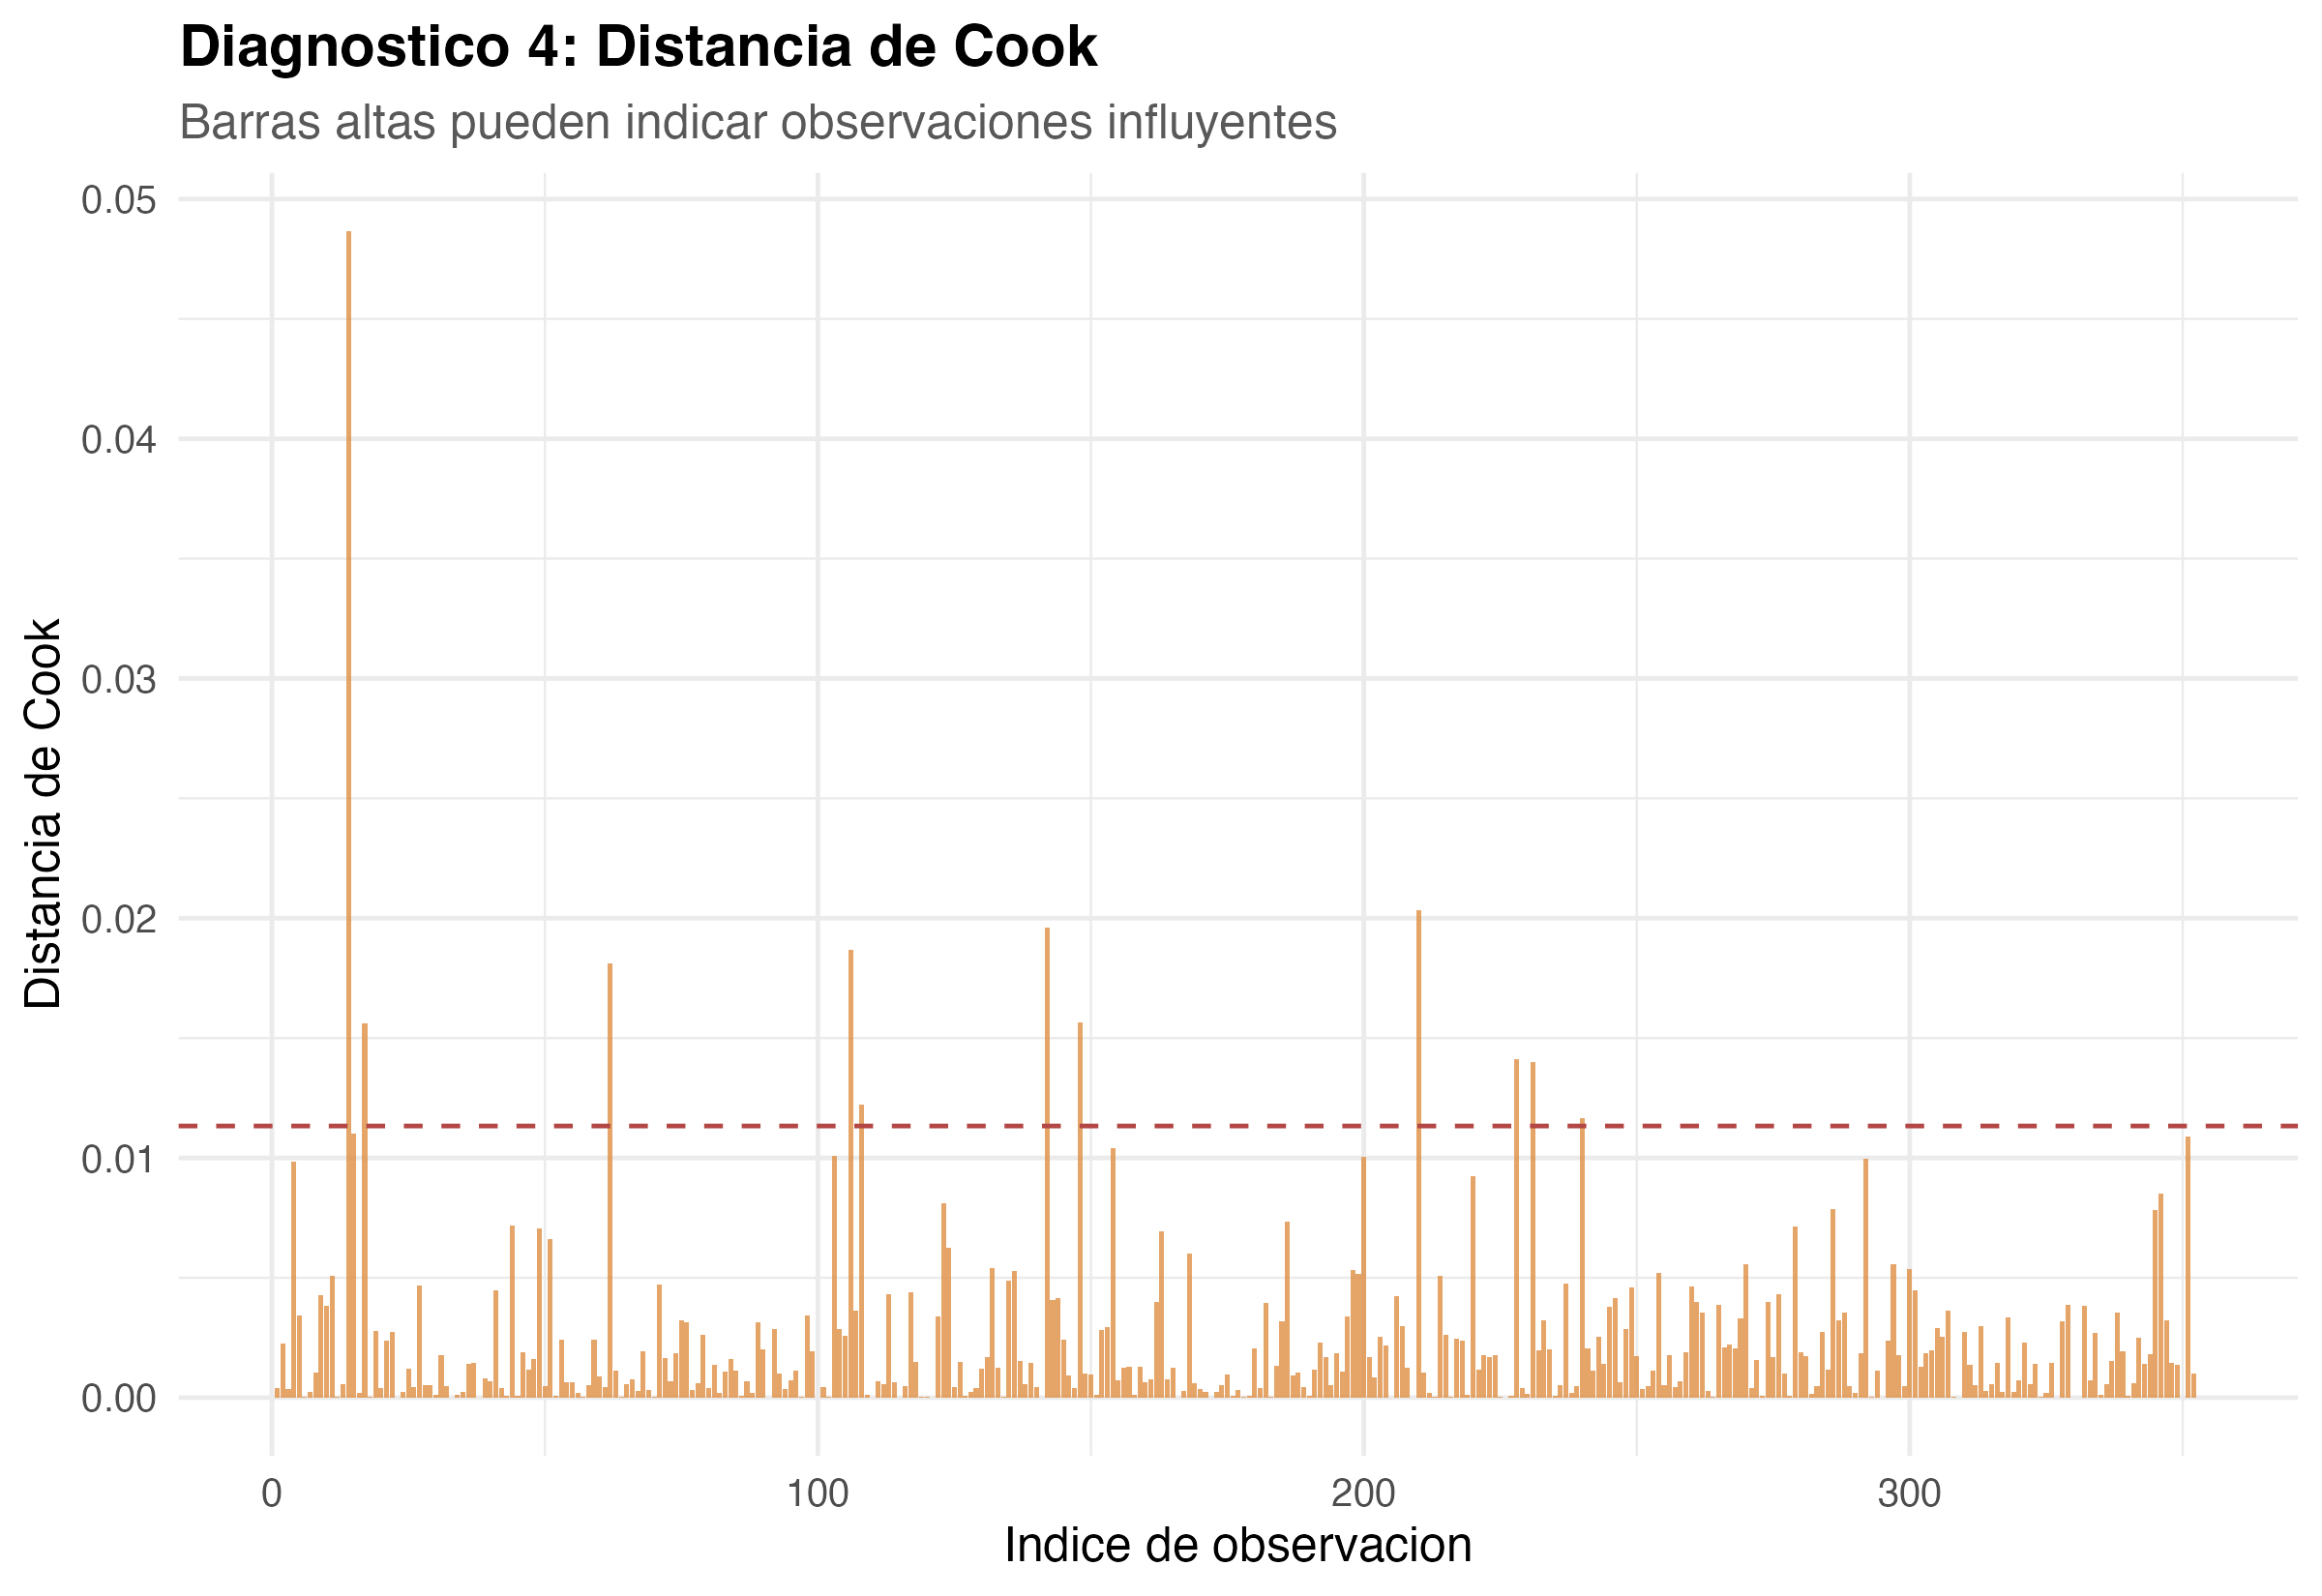
\includegraphics[width=0.7\linewidth]{figuras/diagnostico_04_distancia_cook.png}
    \end{figure}
\end{itemize}

Finalmente, se documentó un análisis fallido. Inicialmente, se consideró usar la red social principal como eje central del análisis, especialmente YouTube, porque podría tener un uso académico. Sin embargo, esta idea se descartó porque la plataforma no indica si el uso fue académico o recreativo. Además, algunas categorías tenían pocos estudiantes, lo que podía producir comparaciones poco confiables. Por esta razón, se decidió dejar la plataforma como una variable secundaria y centrar el análisis en la intensidad de uso, la distracción académica, las horas de estudio y la asistencia.

\subsection{Construcción de fichas de resultados}

A continuación se presentan las fichas de resultados principales obtenidas durante la etapa de modelación. Cada ficha se organiza en dos niveles: primero se describe qué se encontró y luego se interpreta qué significa ese resultado para la pregunta de investigación.

\begin{figure}[H]
    \centering
    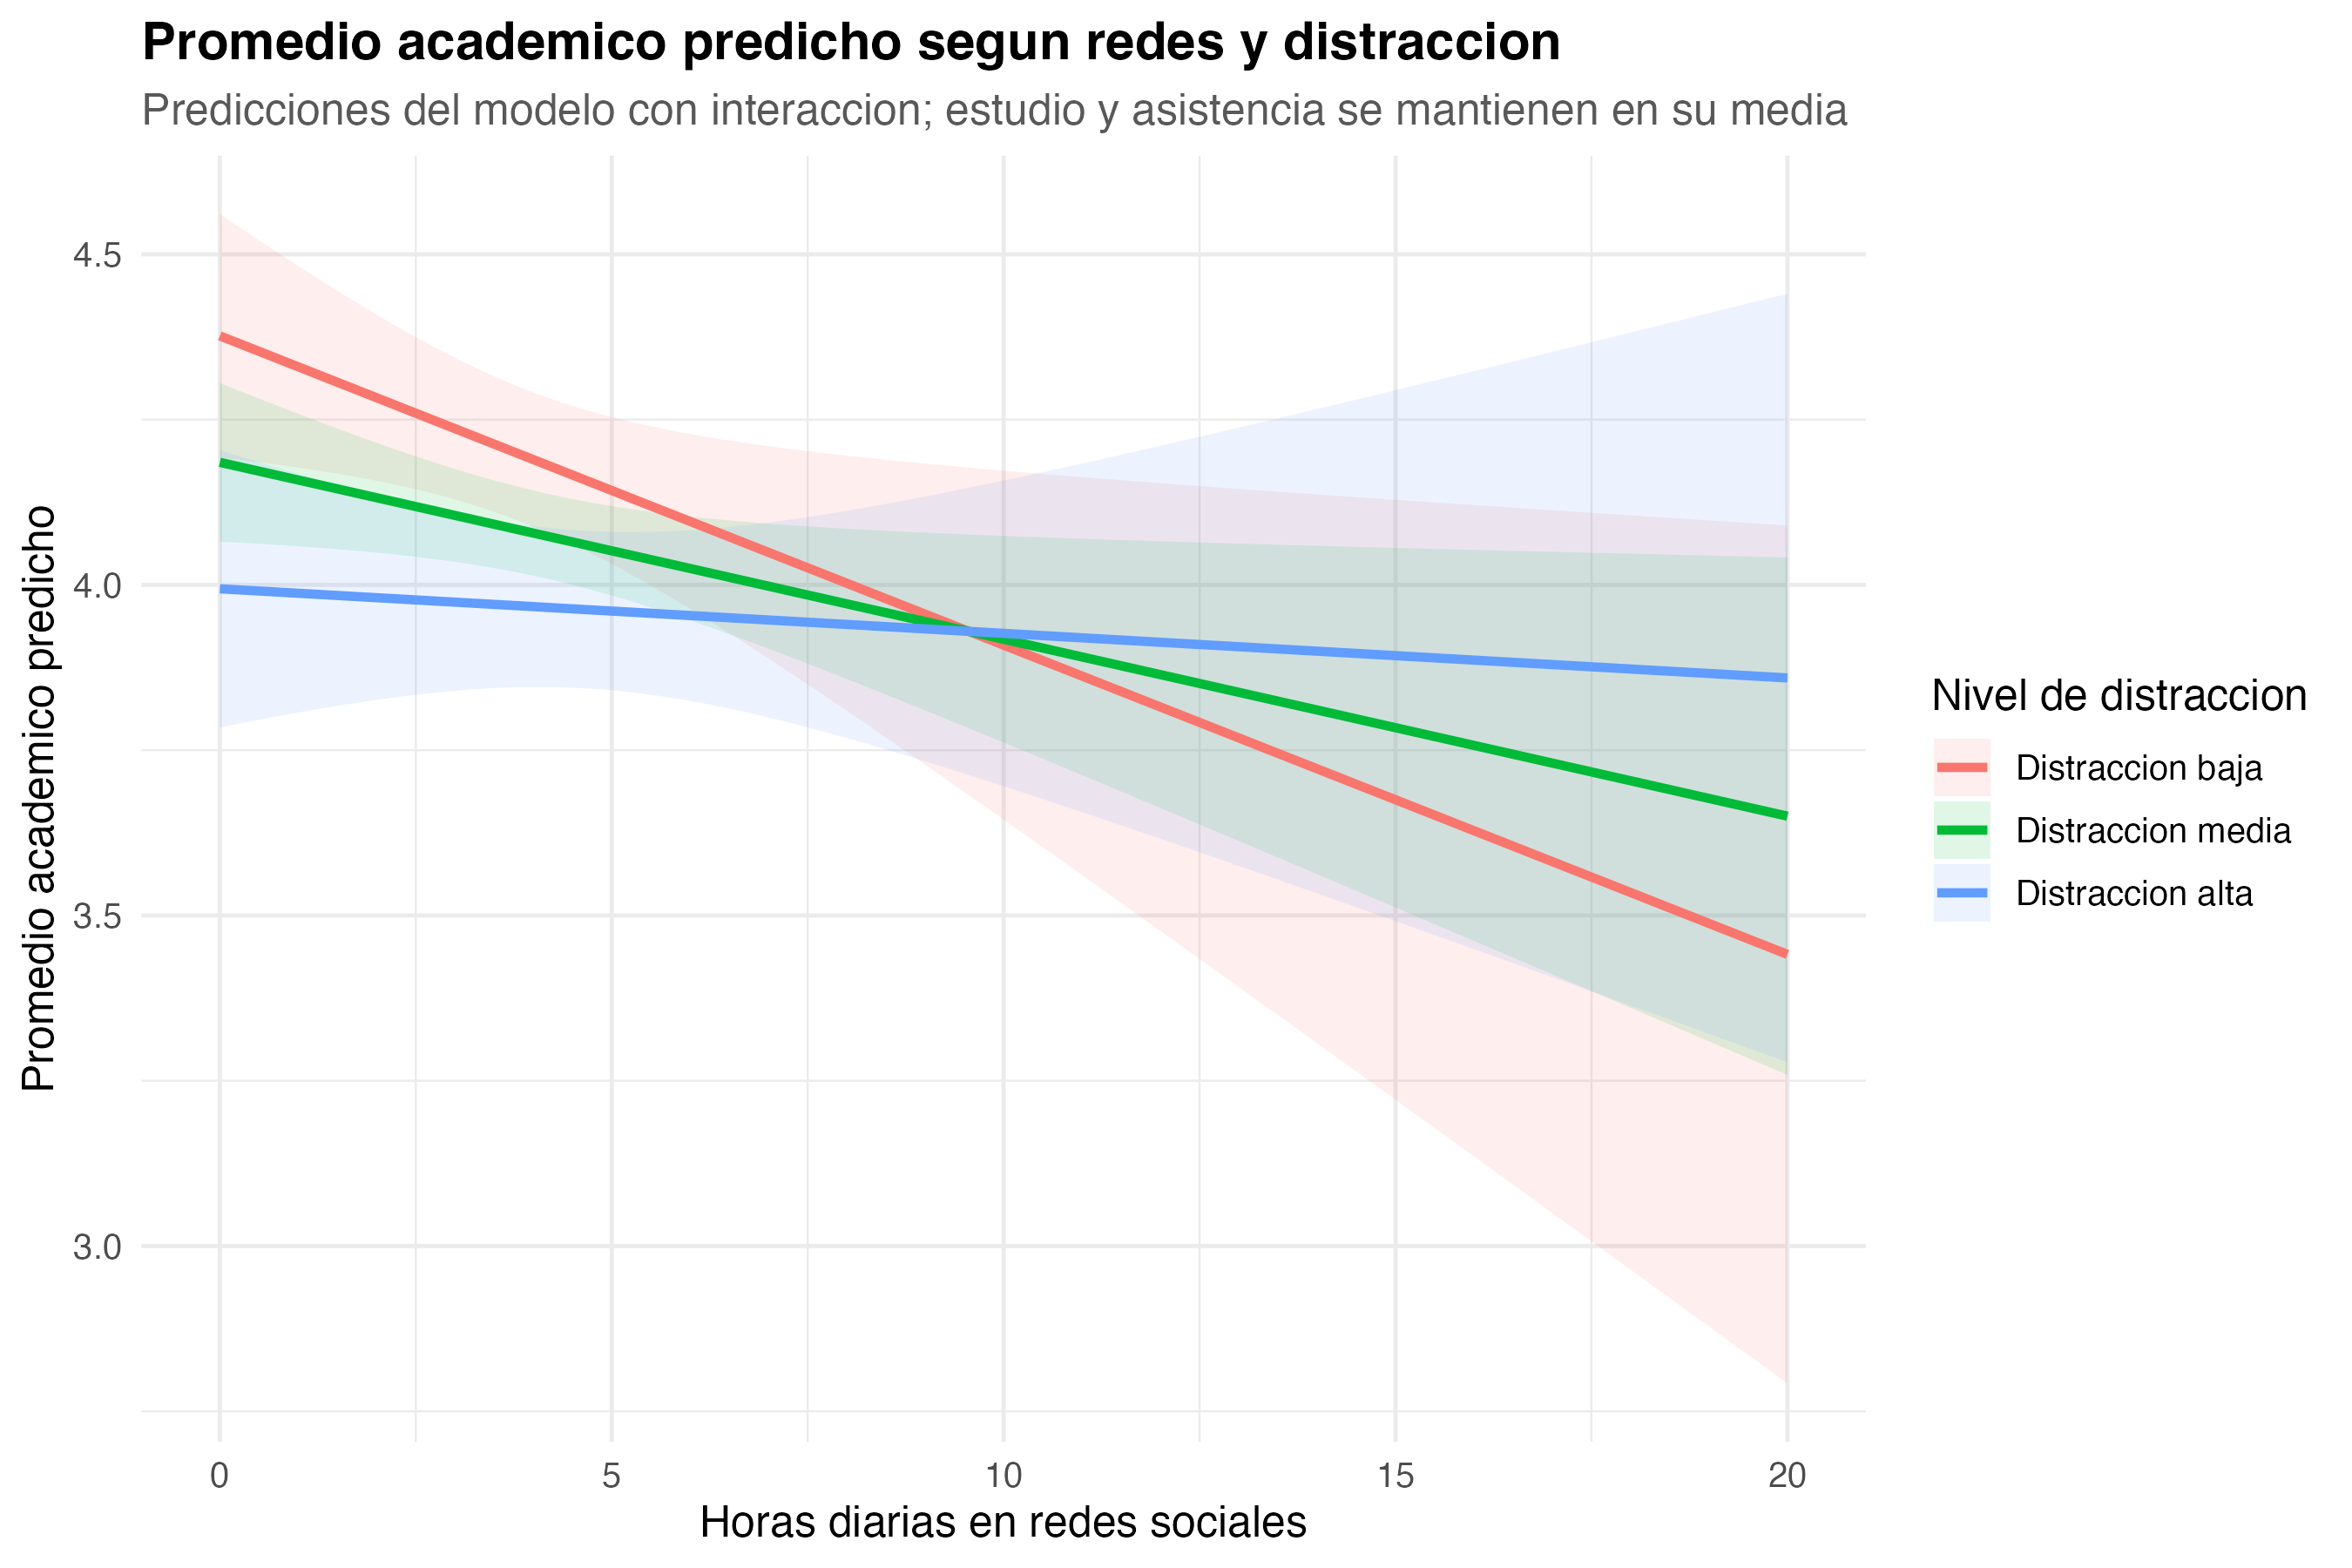
\includegraphics[width=0.82\linewidth]{figuras/figura_06_predicciones_modelo_interaccion.png}
    \caption{Promedio académico predicho según horas en redes sociales y distracción académica}
    \label{fig:predicciones-modelo}
\end{figure}

\subsubsection*{Ficha 1. Prueba t: bajo/moderado uso vs alto uso}

\textbf{Nivel descriptivo: qué encontramos}

\textbf{Titular:} El uso alto muestra menor promedio.

\textbf{Nombre del hallazgo/resultado:} Comparación del promedio académico entre estudiantes con bajo/moderado uso y alto uso de redes sociales.

\textbf{Resumen en una oración:} Los estudiantes con mayor uso tienden a mostrar promedios ligeramente menores.

\textbf{Método o análisis que lo produjo:} Prueba t para dos grupos independientes.

\textbf{Evidencia:} Archivo \texttt{09\_prueba\_t\_grupo\_uso.csv} y comparación entre grupos de uso de redes sociales.

\textbf{Nivel analítico: qué significa}

\textbf{Conexión con la pregunta de investigación:} Este resultado ayuda a responder si el rendimiento académico cambia entre estudiantes con distinto nivel de uso de redes sociales. La prueba permite revisar si la diferencia observada entre grupos es estadísticamente relevante y no solo una diferencia visual.

\textbf{Contraste con la literatura:} Esta ficha se puede comparar con los estudios que plantean que un uso elevado de redes puede relacionarse con menor rendimiento académico. Coincide parcialmente con esa idea, pero el resultado debe interpretarse con cuidado porque el uso de redes no explica todo el promedio.

\textbf{Lo que NO explica este resultado:} No explica si las redes sociales causan un menor promedio. Tampoco explica si el uso fue académico, recreativo o social.

\textbf{Implicación para el siguiente paso:} Fue necesario complementar esta prueba con ANOVA, correlaciones y un modelo que incluyera otras variables académicas.

\subsubsection*{Ficha 2. ANOVA: comparación entre cuatro categorías}

\textbf{Nivel descriptivo: qué encontramos}

\textbf{Titular:} Los grupos no son iguales.

\textbf{Nombre del hallazgo/resultado:} Comparación del promedio académico entre cuatro categorías de uso de redes sociales.

\textbf{Resumen en una oración:} El promedio cambia entre categorías, pero con diferencias moderadas.

\textbf{Método o análisis que lo produjo:} ANOVA de una vía.

\textbf{Evidencia:} Archivo \texttt{10\_anova\_cat\_horas\_redes.csv} y Figura \ref{fig:boxplot-redes}.

\begin{figure}[H]
    \centering
    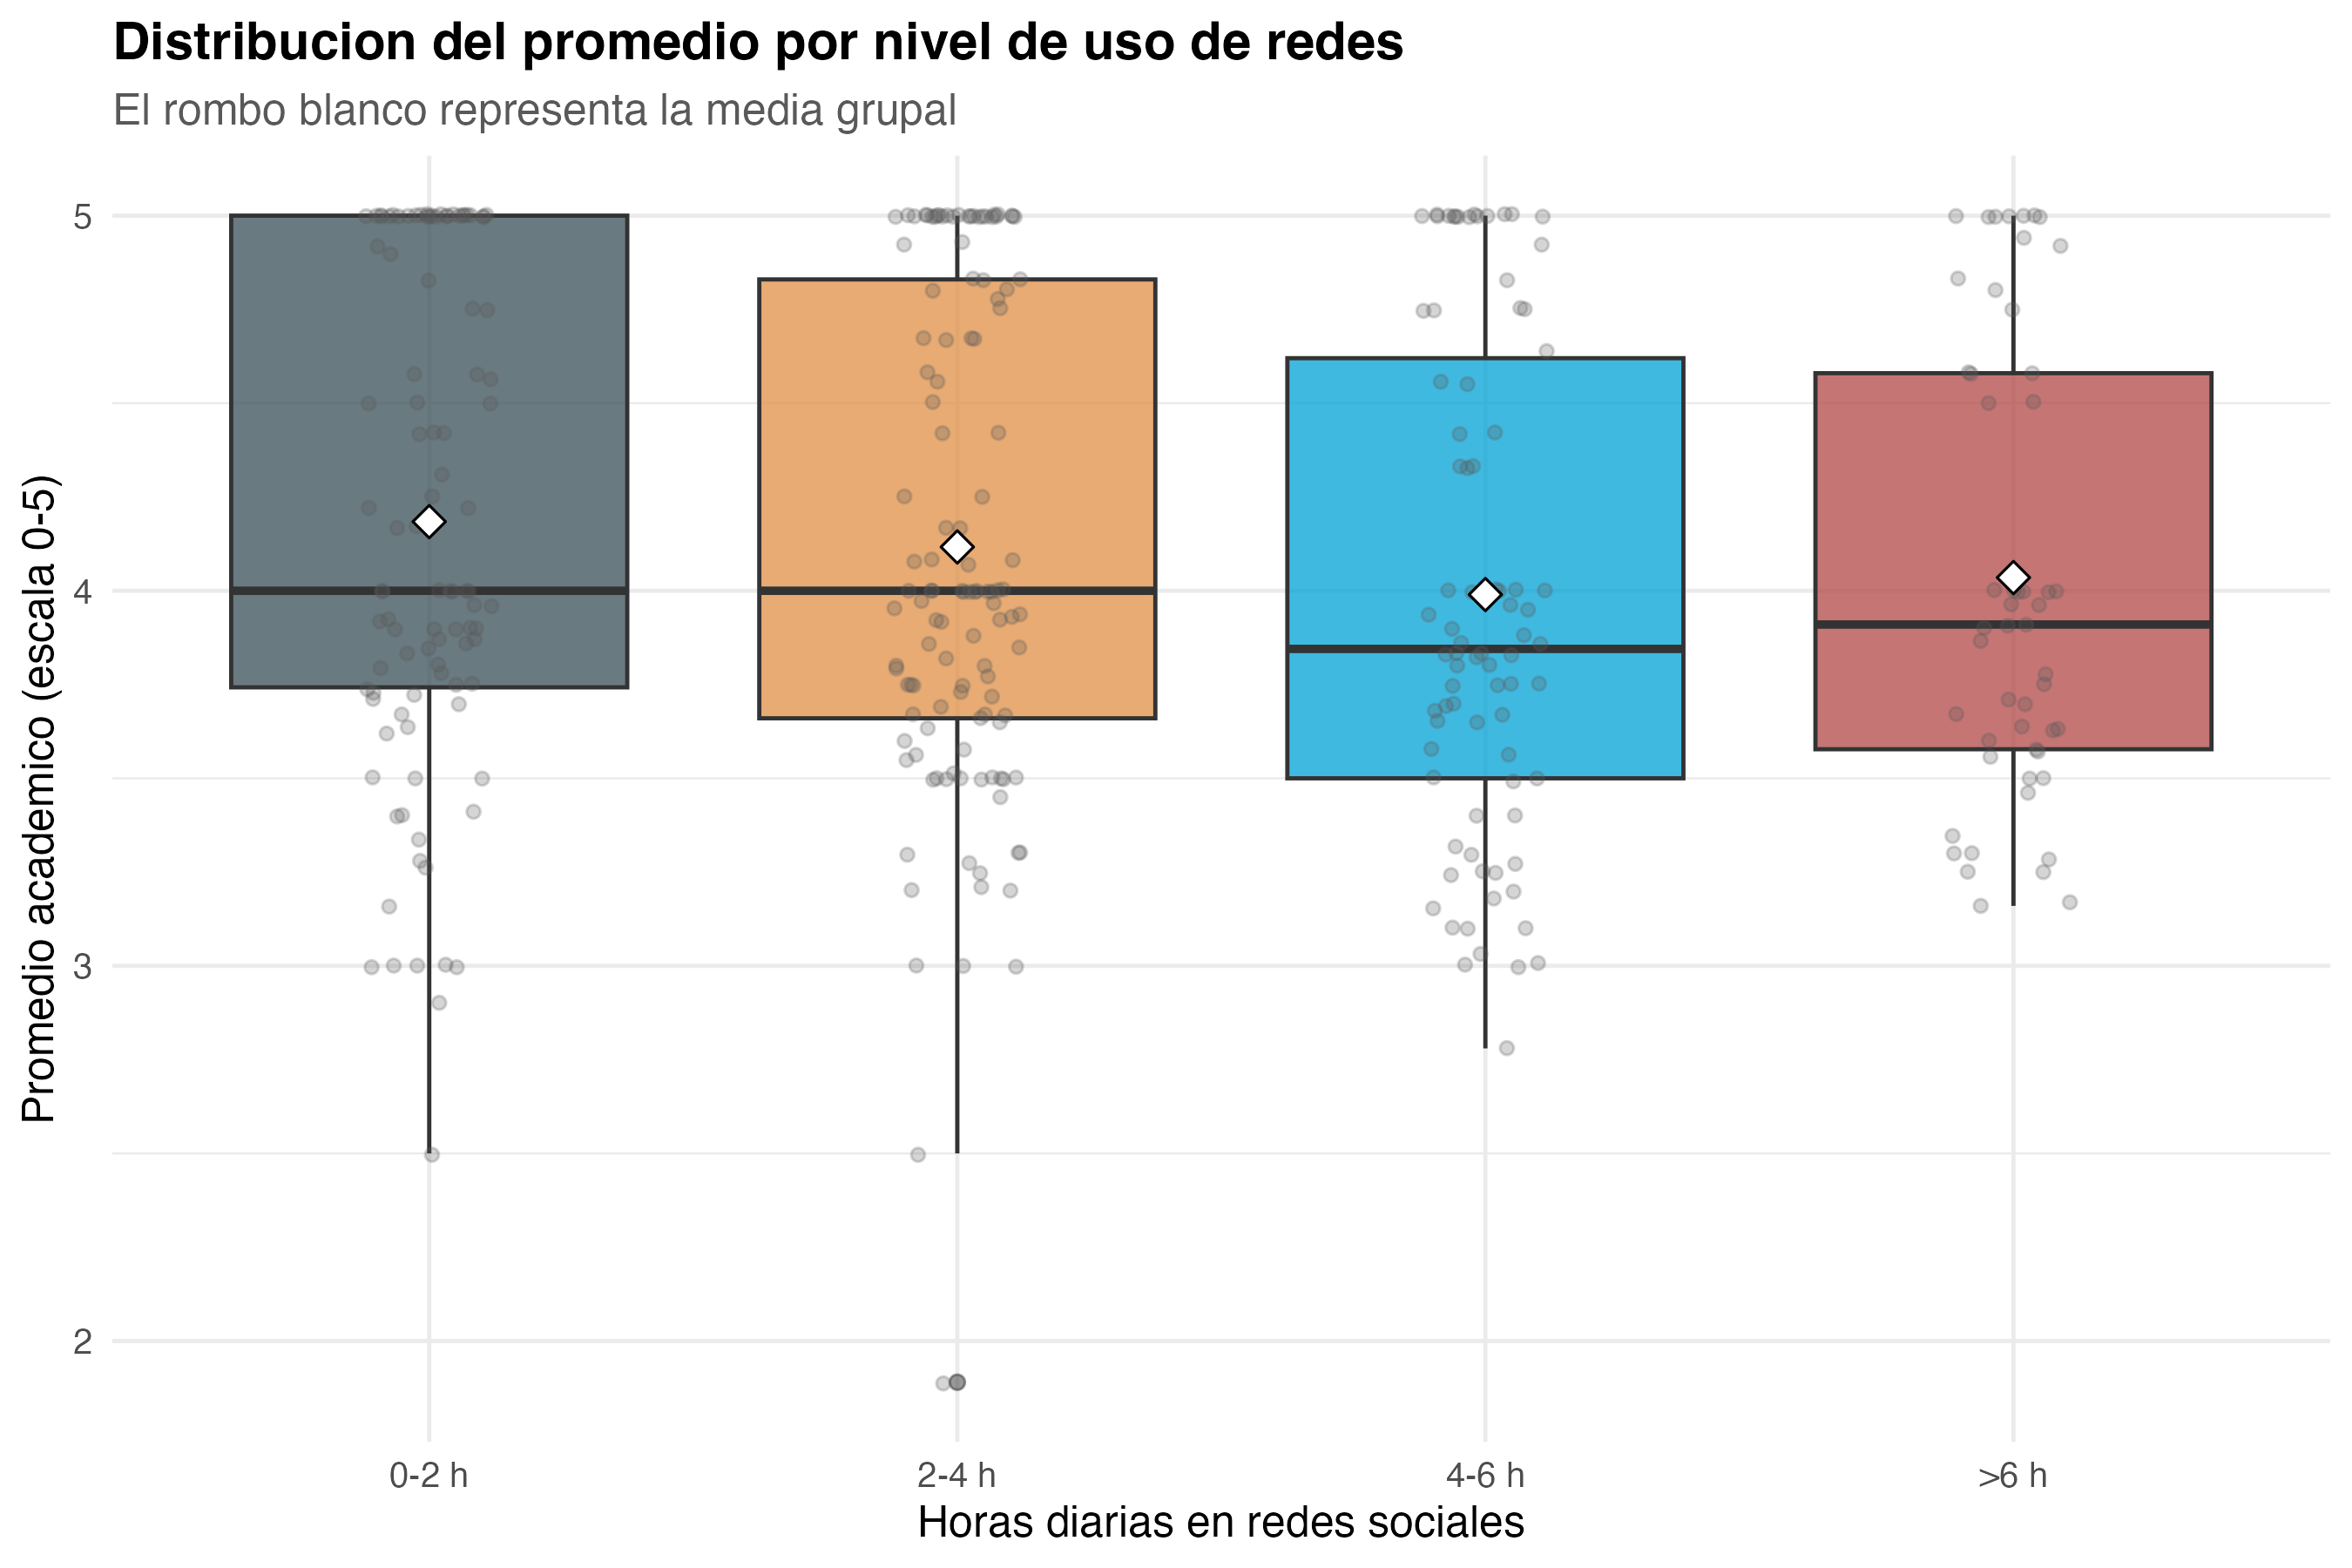
\includegraphics[width=0.72\linewidth]{figuras/figura_02_boxplot_uso_redes.png}
    \caption{Distribución del promedio académico por nivel de uso de redes sociales}
    \label{fig:boxplot-redes}
\end{figure}

\textbf{Nivel analítico: qué significa}

\textbf{Conexión con la pregunta de investigación:} El ANOVA permite evaluar si existen diferencias en el rendimiento académico según el nivel de uso diario de redes sociales. Este análisis es útil porque no reduce el uso de redes a solo dos grupos, sino que permite comparar varios niveles.

\textbf{Contraste con la literatura:} Este resultado se relaciona con la literatura que muestra resultados mixtos. Las diferencias existen, pero no parecen lo suficientemente grandes como para afirmar que el tiempo en redes explique por sí solo el rendimiento académico.

\textbf{Lo que NO explica este resultado:} No indica qué grupo específico causa la diferencia ni explica por qué algunos estudiantes con alto uso mantienen buenos promedios.

\textbf{Implicación para el siguiente paso:} Se necesitó aplicar una prueba no paramétrica como Kruskal-Wallis y luego un modelo con más variables.

\subsubsection*{Ficha 3. Kruskal-Wallis: respaldo no paramétrico}

\textbf{Nivel descriptivo: qué encontramos}

\textbf{Titular:} El respaldo confirma la comparación.

\textbf{Nombre del hallazgo/resultado:} Comparación no paramétrica entre categorías de uso de redes sociales.

\textbf{Resumen en una oración:} Kruskal-Wallis permitió validar la comparación sin exigir normalidad estricta.

\textbf{Método o análisis que lo produjo:} Prueba de Kruskal-Wallis.

\textbf{Evidencia:} Archivo \texttt{11\_kruskal\_cat\_horas\_redes.csv}.

\textbf{Nivel analítico: qué significa}

\textbf{Conexión con la pregunta de investigación:} Esta prueba refuerza el análisis porque permite comparar los grupos de uso de redes sociales aun cuando los supuestos del ANOVA no se cumplan completamente. Esto hace que la respuesta a la pregunta de investigación sea más prudente.

\textbf{Contraste con la literatura:} Esta ficha no se compara directamente con un autor específico, sino que fortalece la validez del análisis estadístico usado para contrastar los patrones observados.

\textbf{Lo que NO explica este resultado:} No mide el tamaño exacto del efecto ni indica causalidad. Solo permite evaluar si existen diferencias entre los grupos.

\textbf{Implicación para el siguiente paso:} Ayudó a decidir que las conclusiones debían apoyarse en más de una prueba y no solo en el ANOVA.

\subsubsection*{Ficha 4. Pearson: horas en redes vs promedio}

\textbf{Nivel descriptivo: qué encontramos}

\textbf{Titular:} Más redes, menor promedio.

\textbf{Nombre del hallazgo/resultado:} Asociación lineal entre horas diarias en redes sociales y promedio académico.

\textbf{Resumen en una oración:} Las horas en redes se asocian negativamente con el promedio académico.

\textbf{Método o análisis que lo produjo:} Correlación de Pearson.

\textbf{Evidencia:} Archivo \texttt{08\_correlaciones\_horas\_redes\_promedio.csv} y Figura \ref{fig:redes-promedio}.

\begin{figure}[H]
    \centering
    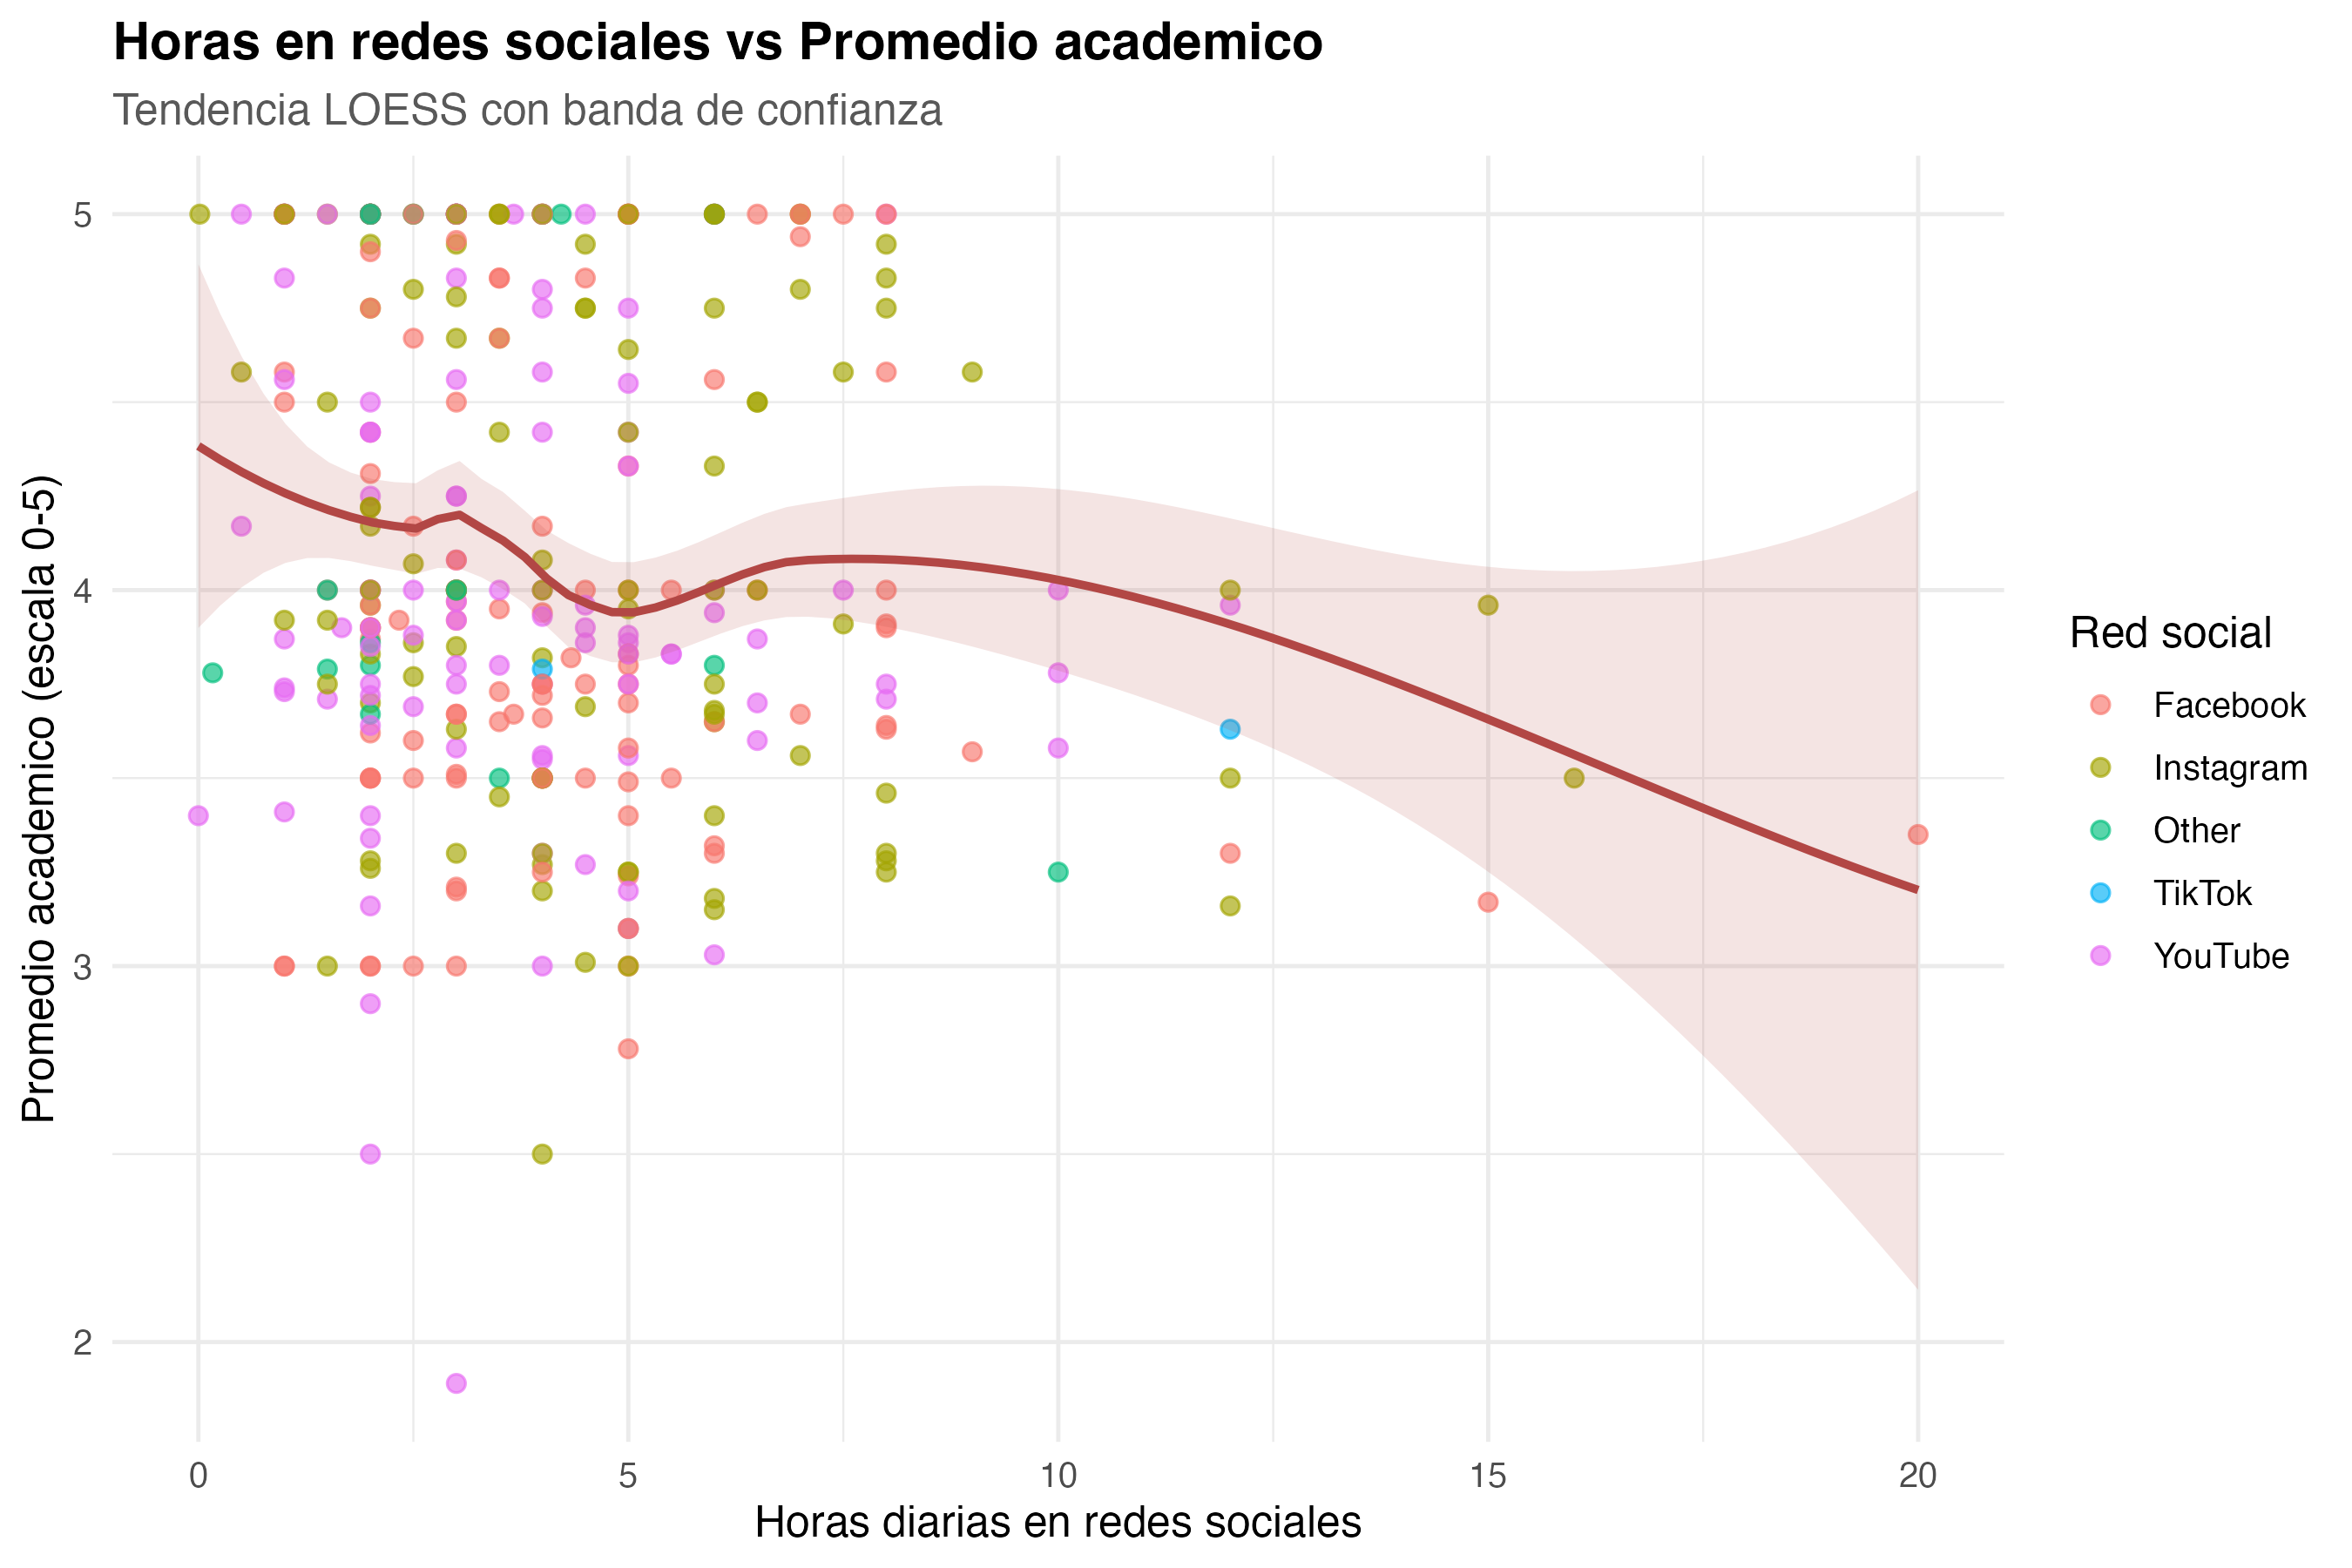
\includegraphics[width=0.75\linewidth]{figuras/figura_01_horas_redes_vs_promedio.png}
    \caption{Horas en redes sociales y promedio académico}
    \label{fig:redes-promedio}
\end{figure}

\textbf{Nivel analítico: qué significa}

\textbf{Conexión con la pregunta de investigación:} Esta ficha conecta directamente con la pregunta principal, porque analiza si el tiempo en redes sociales se relaciona con el rendimiento académico. La tendencia observada es negativa, aunque no totalmente fuerte.

\textbf{Contraste con la literatura:} Esta ficha coincide parcialmente con autores que señalan que el uso elevado de redes puede afectar el rendimiento. Sin embargo, también coincide con estudios de resultados mixtos, porque la relación no es perfecta ni explica todos los casos.

\textbf{Lo que NO explica este resultado:} No explica el tipo de uso de redes sociales ni si el estudiante usa esas plataformas para estudiar, entretenerse o comunicarse.

\textbf{Implicación para el siguiente paso:} Fue necesario incluir variables como distracción académica, horas de estudio y asistencia.

\subsubsection*{Ficha 5. Spearman: horas en redes vs promedio}

\textbf{Nivel descriptivo: qué encontramos}

\textbf{Titular:} La relación no es perfectamente lineal.

\textbf{Nombre del hallazgo/resultado:} Asociación monotónica entre horas en redes sociales y promedio académico.

\textbf{Resumen en una oración:} Spearman confirma que la relación no depende solo de linealidad.

\textbf{Método o análisis que lo produjo:} Correlación de Spearman.

\textbf{Evidencia:} Archivo \texttt{08\_correlaciones\_horas\_redes\_promedio.csv}.

\textbf{Nivel analítico: qué significa}

\textbf{Conexión con la pregunta de investigación:} Esta prueba ayuda a revisar la relación entre redes sociales y rendimiento sin asumir que la relación debe ser completamente lineal. Esto es importante porque los gráficos mostraron una relación irregular.

\textbf{Contraste con la literatura:} Esta ficha se relaciona con los estudios que muestran resultados no concluyentes. El uso de redes puede tener relación con el promedio, pero esa relación no se comporta igual para todos los estudiantes.

\textbf{Lo que NO explica este resultado:} No explica diferencias individuales, como organización del tiempo, dificultad de los cursos o motivación académica.

\textbf{Implicación para el siguiente paso:} Confirmó que era necesario construir una interpretación más completa y no basarse únicamente en una correlación simple.

\subsubsection*{Ficha 6. Pearson: horas de estudio vs promedio}

\textbf{Nivel descriptivo: qué encontramos}

\textbf{Titular:} Estudiar más ayuda al promedio.

\textbf{Nombre del hallazgo/resultado:} Asociación entre horas de estudio y promedio académico.

\textbf{Resumen en una oración:} Más horas de estudio se asocian con mejores promedios académicos.

\textbf{Método o análisis que lo produjo:} Correlación de Pearson y modelo de regresión.

\textbf{Evidencia:} Figura \ref{fig:estudio-promedio} y coeficiente positivo de \texttt{horas\_estudio} en el modelo seleccionado.

\begin{figure}[H]
    \centering
    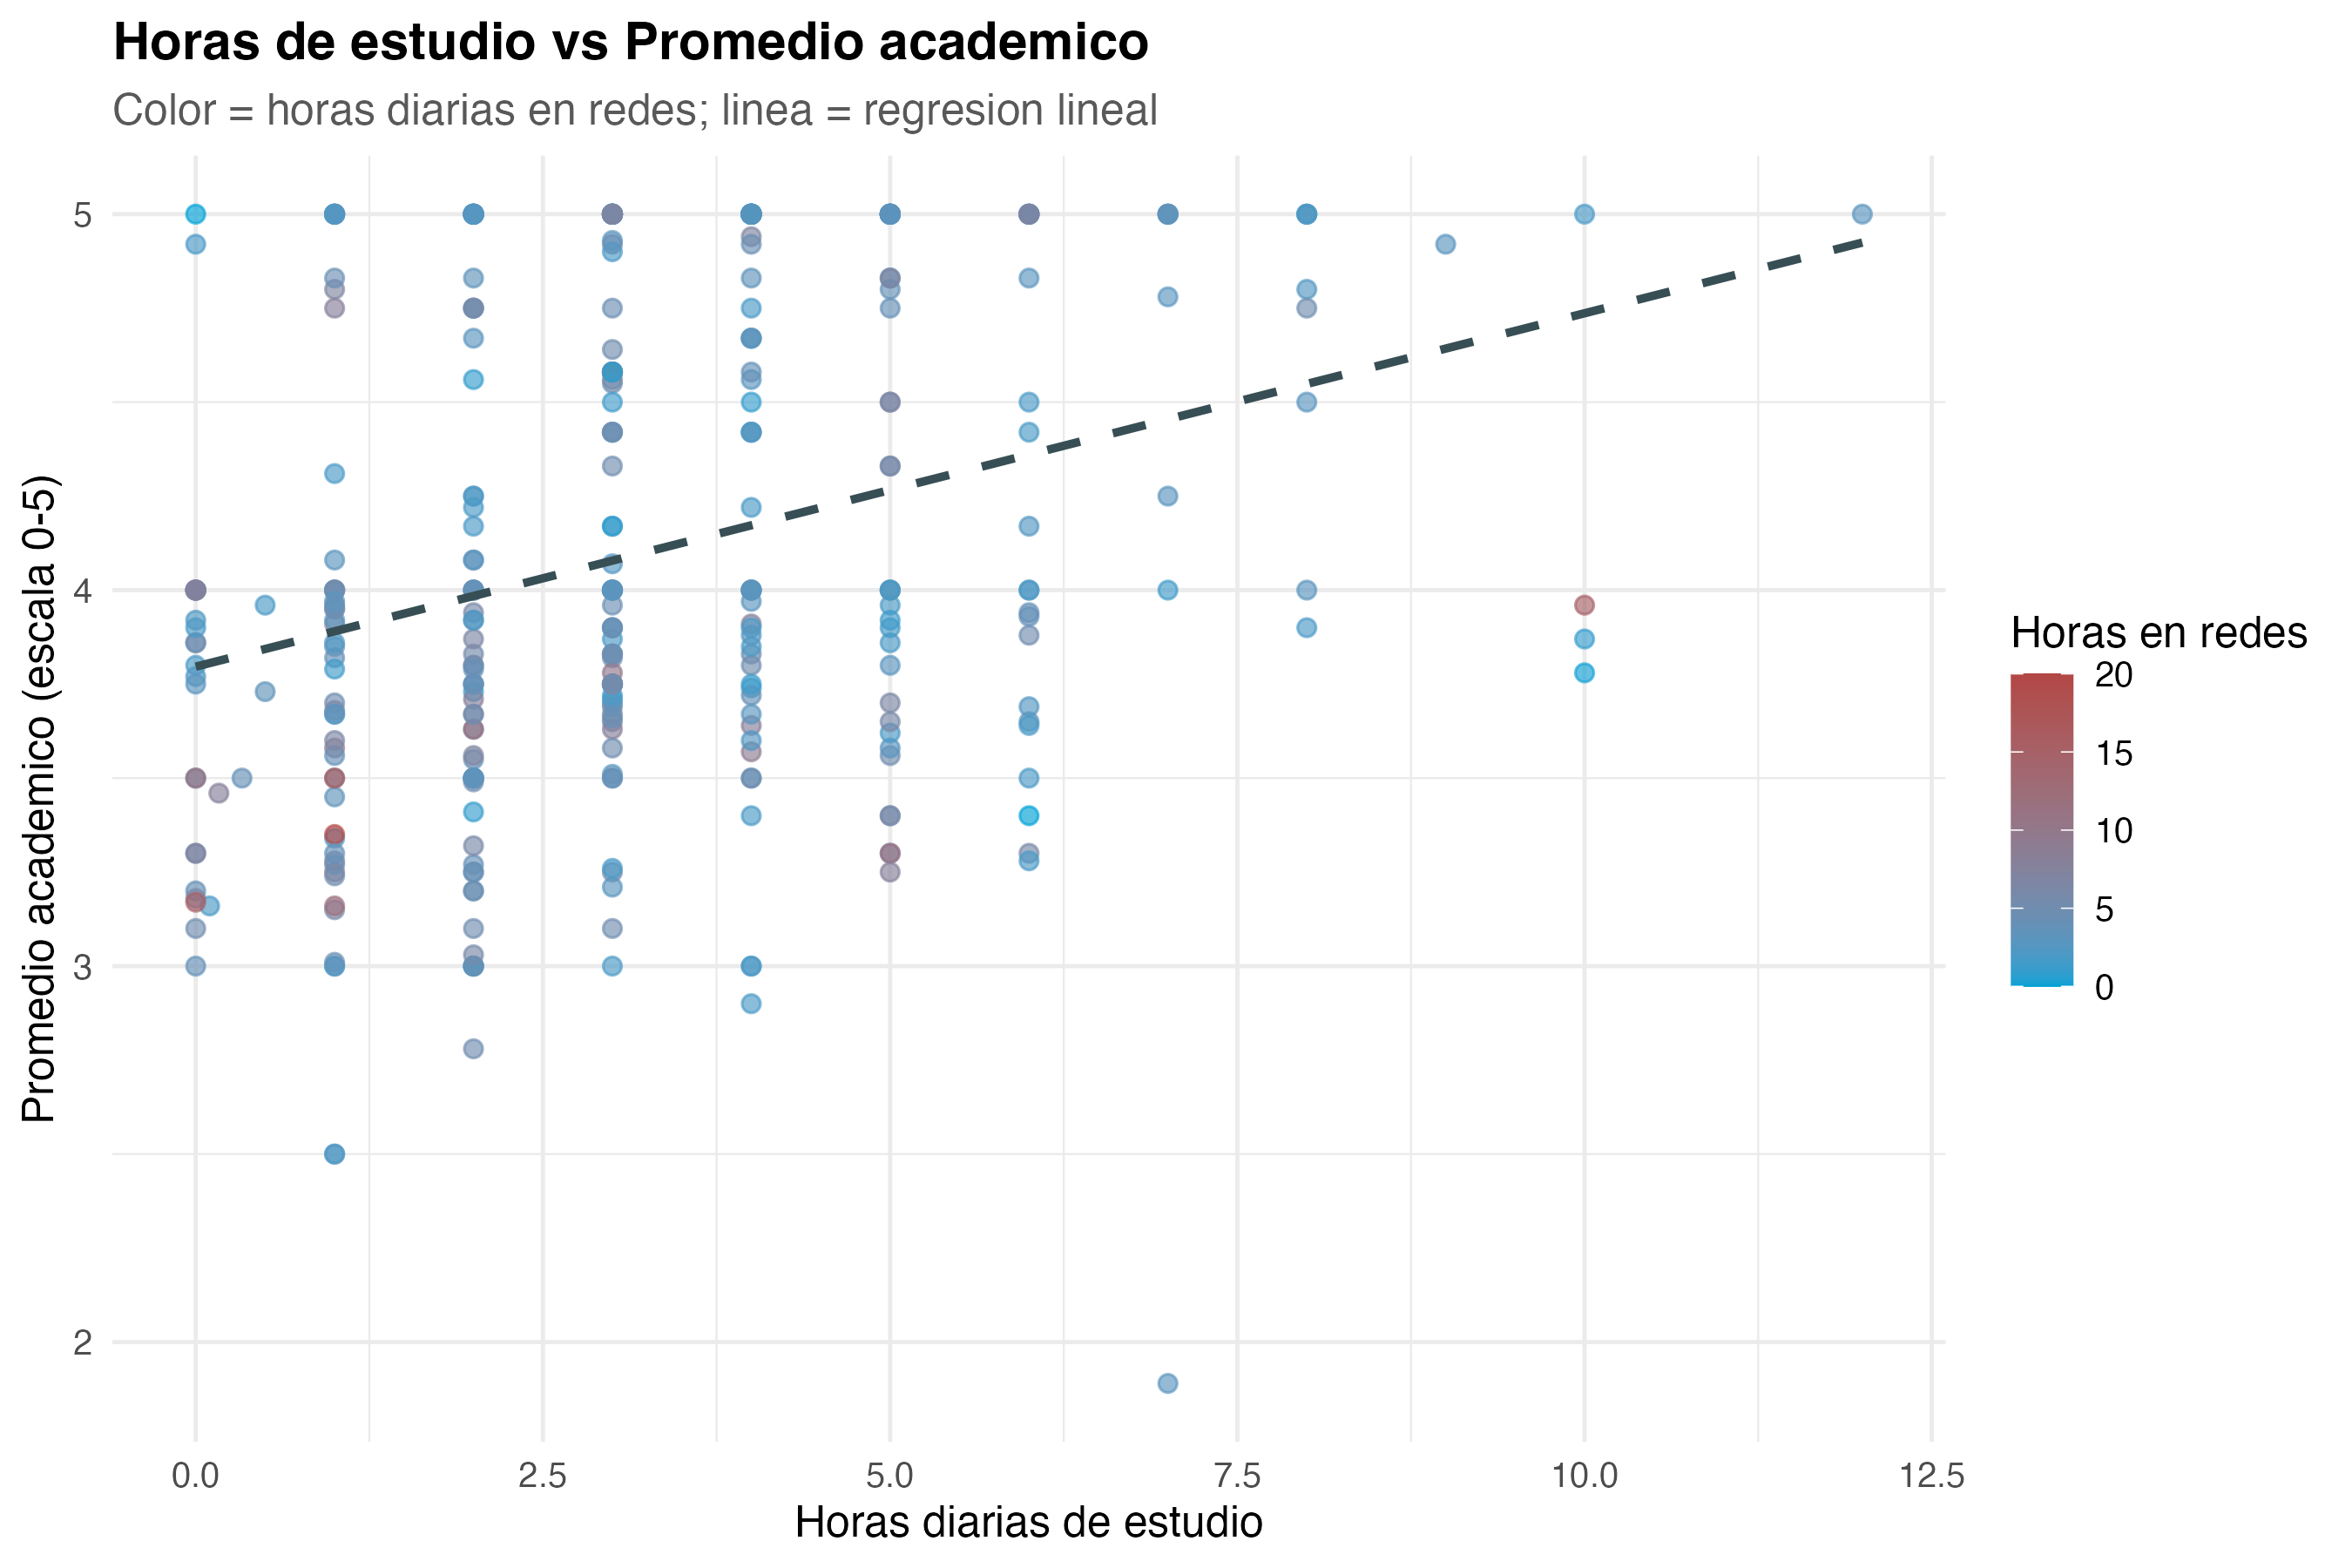
\includegraphics[width=0.75\linewidth]{figuras/figura_03_horas_estudio_vs_promedio.png}
    \caption{Horas de estudio y promedio académico}
    \label{fig:estudio-promedio}
\end{figure}

\textbf{Nivel analítico: qué significa}

\textbf{Conexión con la pregunta de investigación:} Este resultado muestra que el rendimiento académico no debe explicarse únicamente por el uso de redes sociales. Las horas de estudio también tienen un papel importante en el promedio.

\textbf{Contraste con la literatura:} Este resultado coincide con la idea general de que el rendimiento académico es multifactorial. No contradice la literatura sobre redes sociales, sino que ayuda a explicar por qué el tiempo en redes no es suficiente para entender el rendimiento.

\textbf{Lo que NO explica este resultado:} No mide la calidad del estudio. Un estudiante puede estudiar muchas horas, pero con baja concentración o poca organización.

\textbf{Implicación para el siguiente paso:} Se incorporó esta variable dentro del modelo seleccionado para controlar parcialmente los hábitos académicos.

\subsubsection*{Ficha 7. Distracción académica vs promedio}

\textbf{Nivel descriptivo: qué encontramos}

\textbf{Titular:} La distracción sí importa.

\textbf{Nombre del hallazgo/resultado:} Asociación entre distracción académica y promedio académico.

\textbf{Resumen en una oración:} Mayor distracción académica se relaciona con menor promedio académico.

\textbf{Método o análisis que lo produjo:} Correlación y modelo de regresión.

\textbf{Evidencia:} Figura \ref{fig:heatmap-redes-distraccion} y coeficiente negativo de \texttt{distraccion\_acad} en el modelo seleccionado.

\begin{figure}[H]
    \centering
    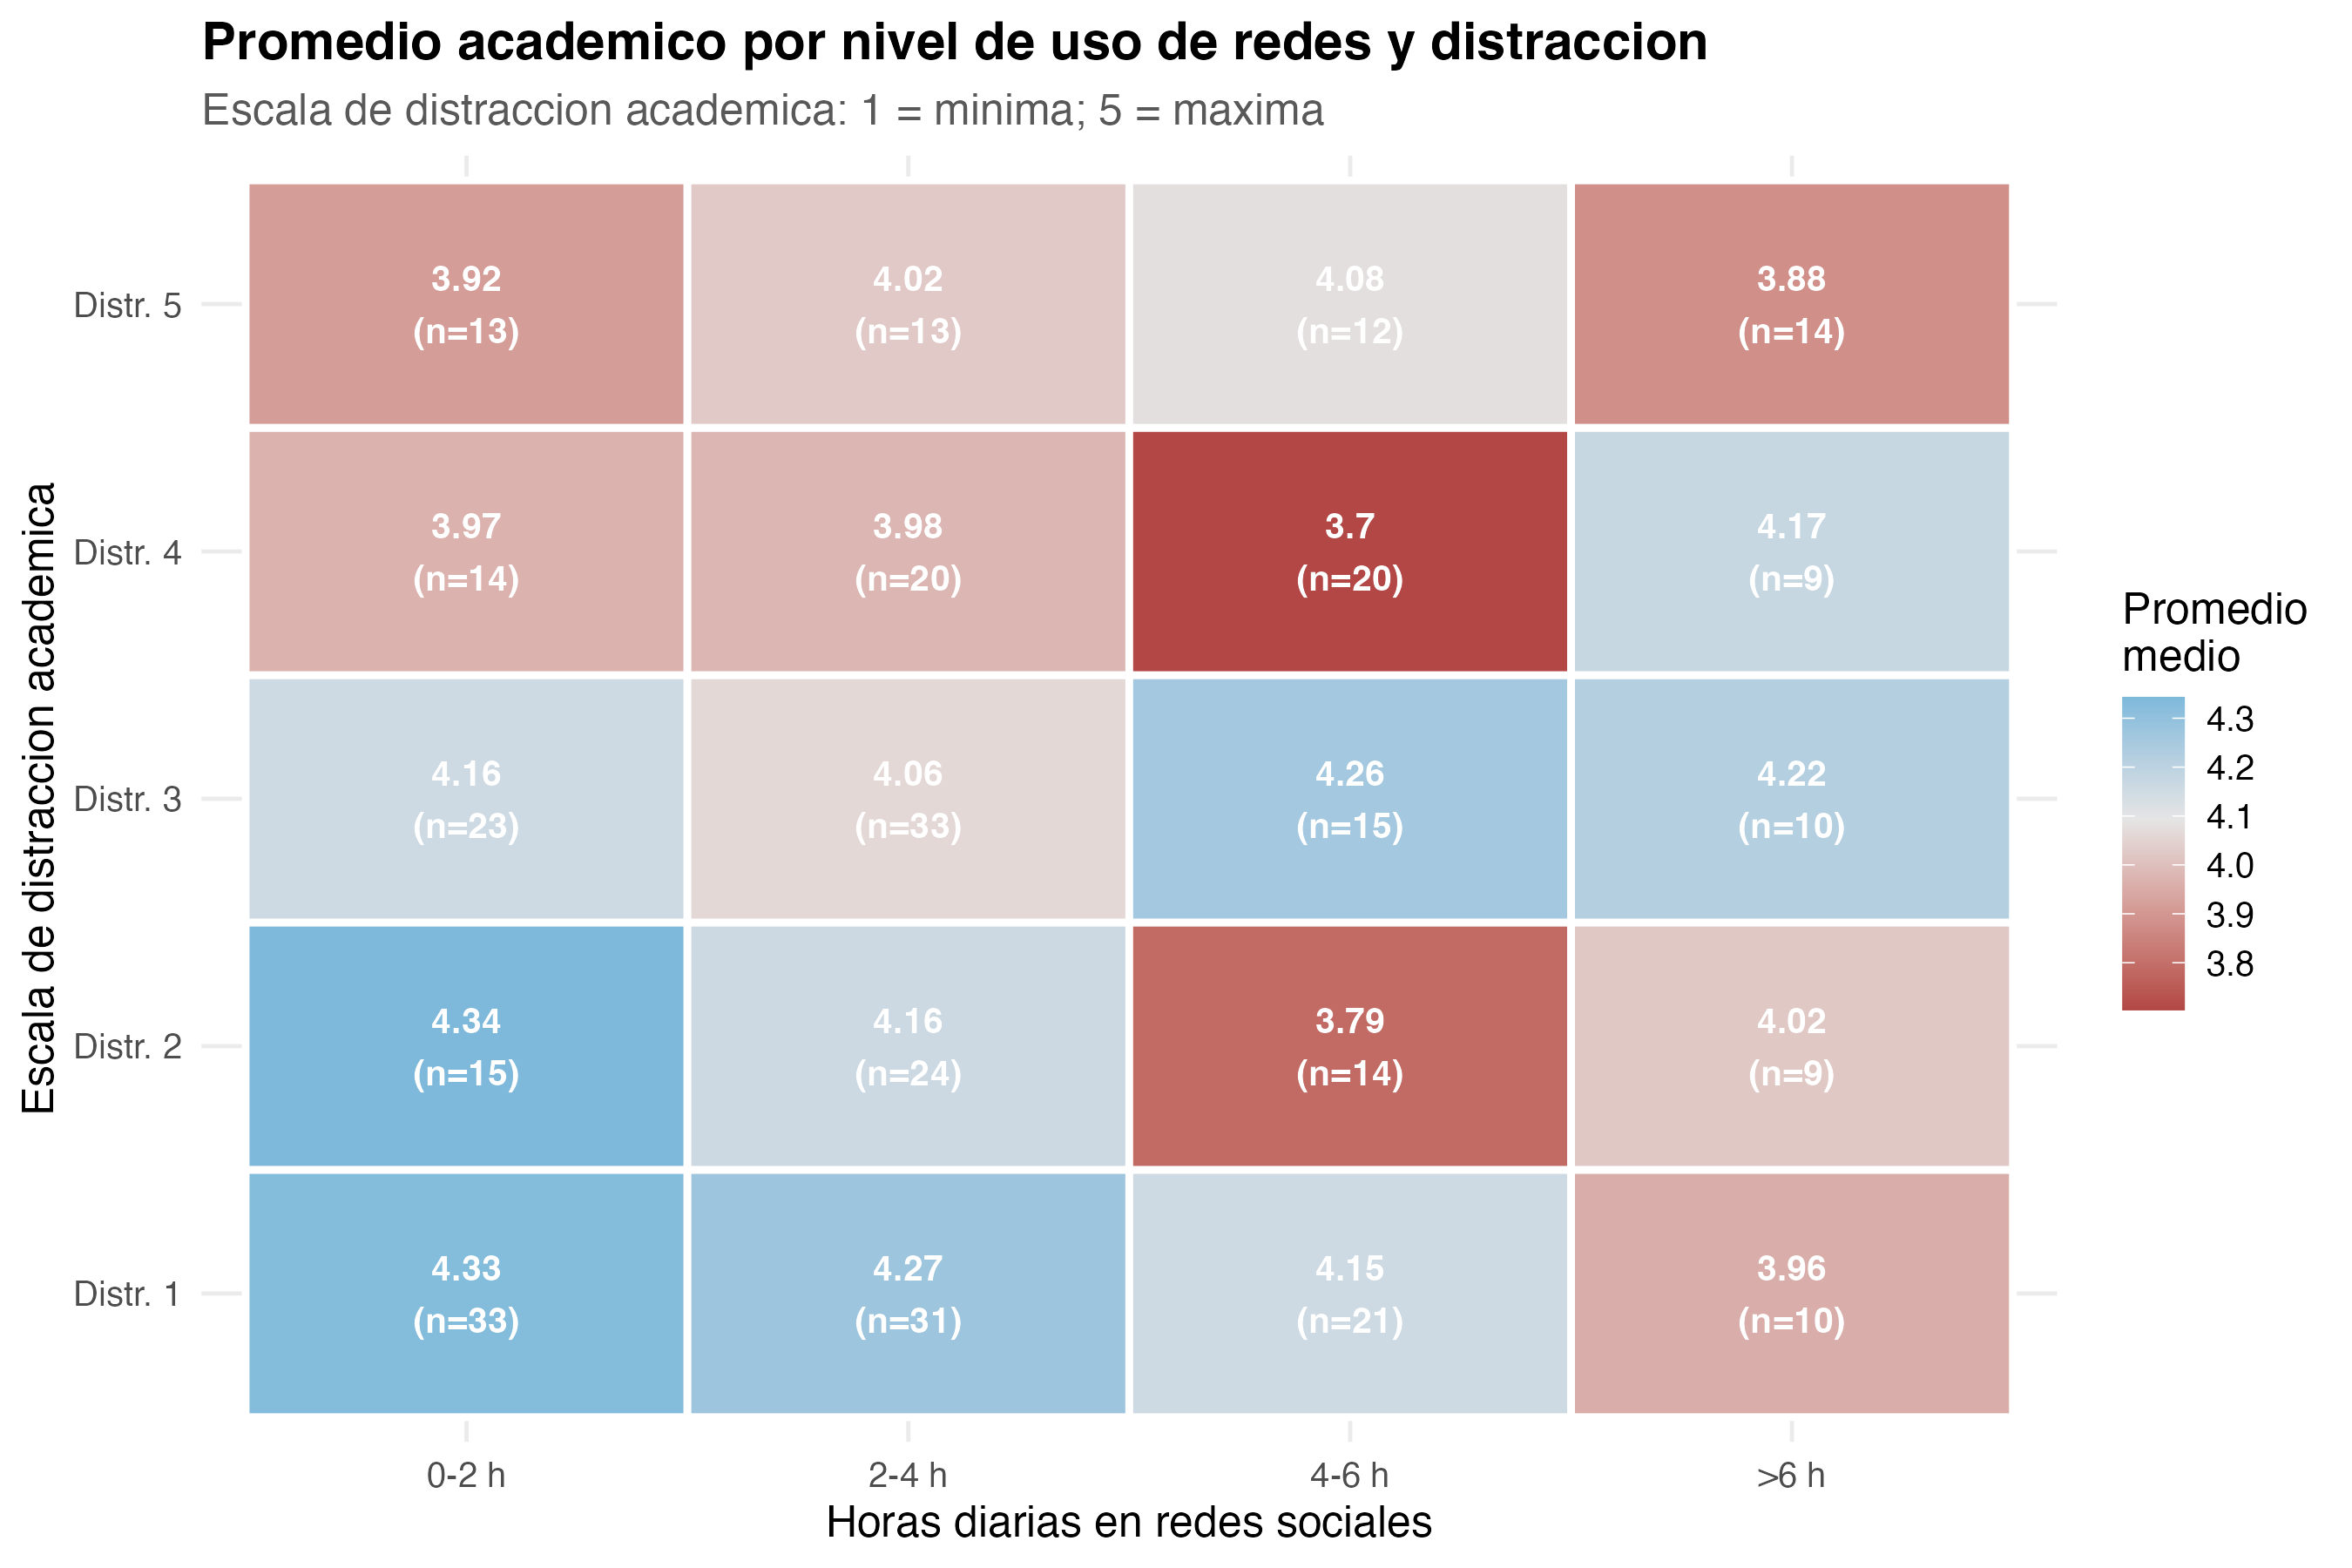
\includegraphics[width=0.78\linewidth]{figuras/figura_05_heatmap_redes_distraccion.png}
    \caption{Promedio académico por nivel de uso de redes y distracción}
    \label{fig:heatmap-redes-distraccion}
\end{figure}

\textbf{Nivel analítico: qué significa}

\textbf{Conexión con la pregunta de investigación:} Esta ficha es una de las más importantes, porque muestra que no solo importa cuánto tiempo se usan las redes sociales, sino también si ese uso interrumpe el estudio. Esto permite entender mejor la relación entre redes y rendimiento.

\textbf{Contraste con la literatura:} Esta ficha coincide con autores que señalan que el uso de redes puede afectar la concentración. También ayuda a explicar por qué algunos estudios no encuentran una relación directa entre tiempo en redes y rendimiento.

\textbf{Lo que NO explica este resultado:} No demuestra que la distracción sea causada únicamente por redes sociales. La distracción también puede venir de otros factores personales, familiares o académicos.

\textbf{Implicación para el siguiente paso:} La distracción académica se mantuvo como variable principal dentro del modelo final.

\subsubsection*{Ficha 8. Diagnóstico del modelo}

\textbf{Nivel descriptivo: qué encontramos}

\textbf{Titular:} El modelo requiere cautela.

\textbf{Nombre del hallazgo/resultado:} Revisión gráfica de los supuestos y valores influyentes del modelo.

\textbf{Resumen en una oración:} Los diagnósticos permiten interpretar el modelo con precaución razonable.

\textbf{Método o análisis que lo produjo:} Gráficos de residuos, QQ plot, histograma de residuos y distancia de Cook.

\textbf{Evidencia:} Figuras \ref{fig:diagnostico-residuos} y \ref{fig:diagnostico-qq}.

\begin{figure}[H]
    \centering
    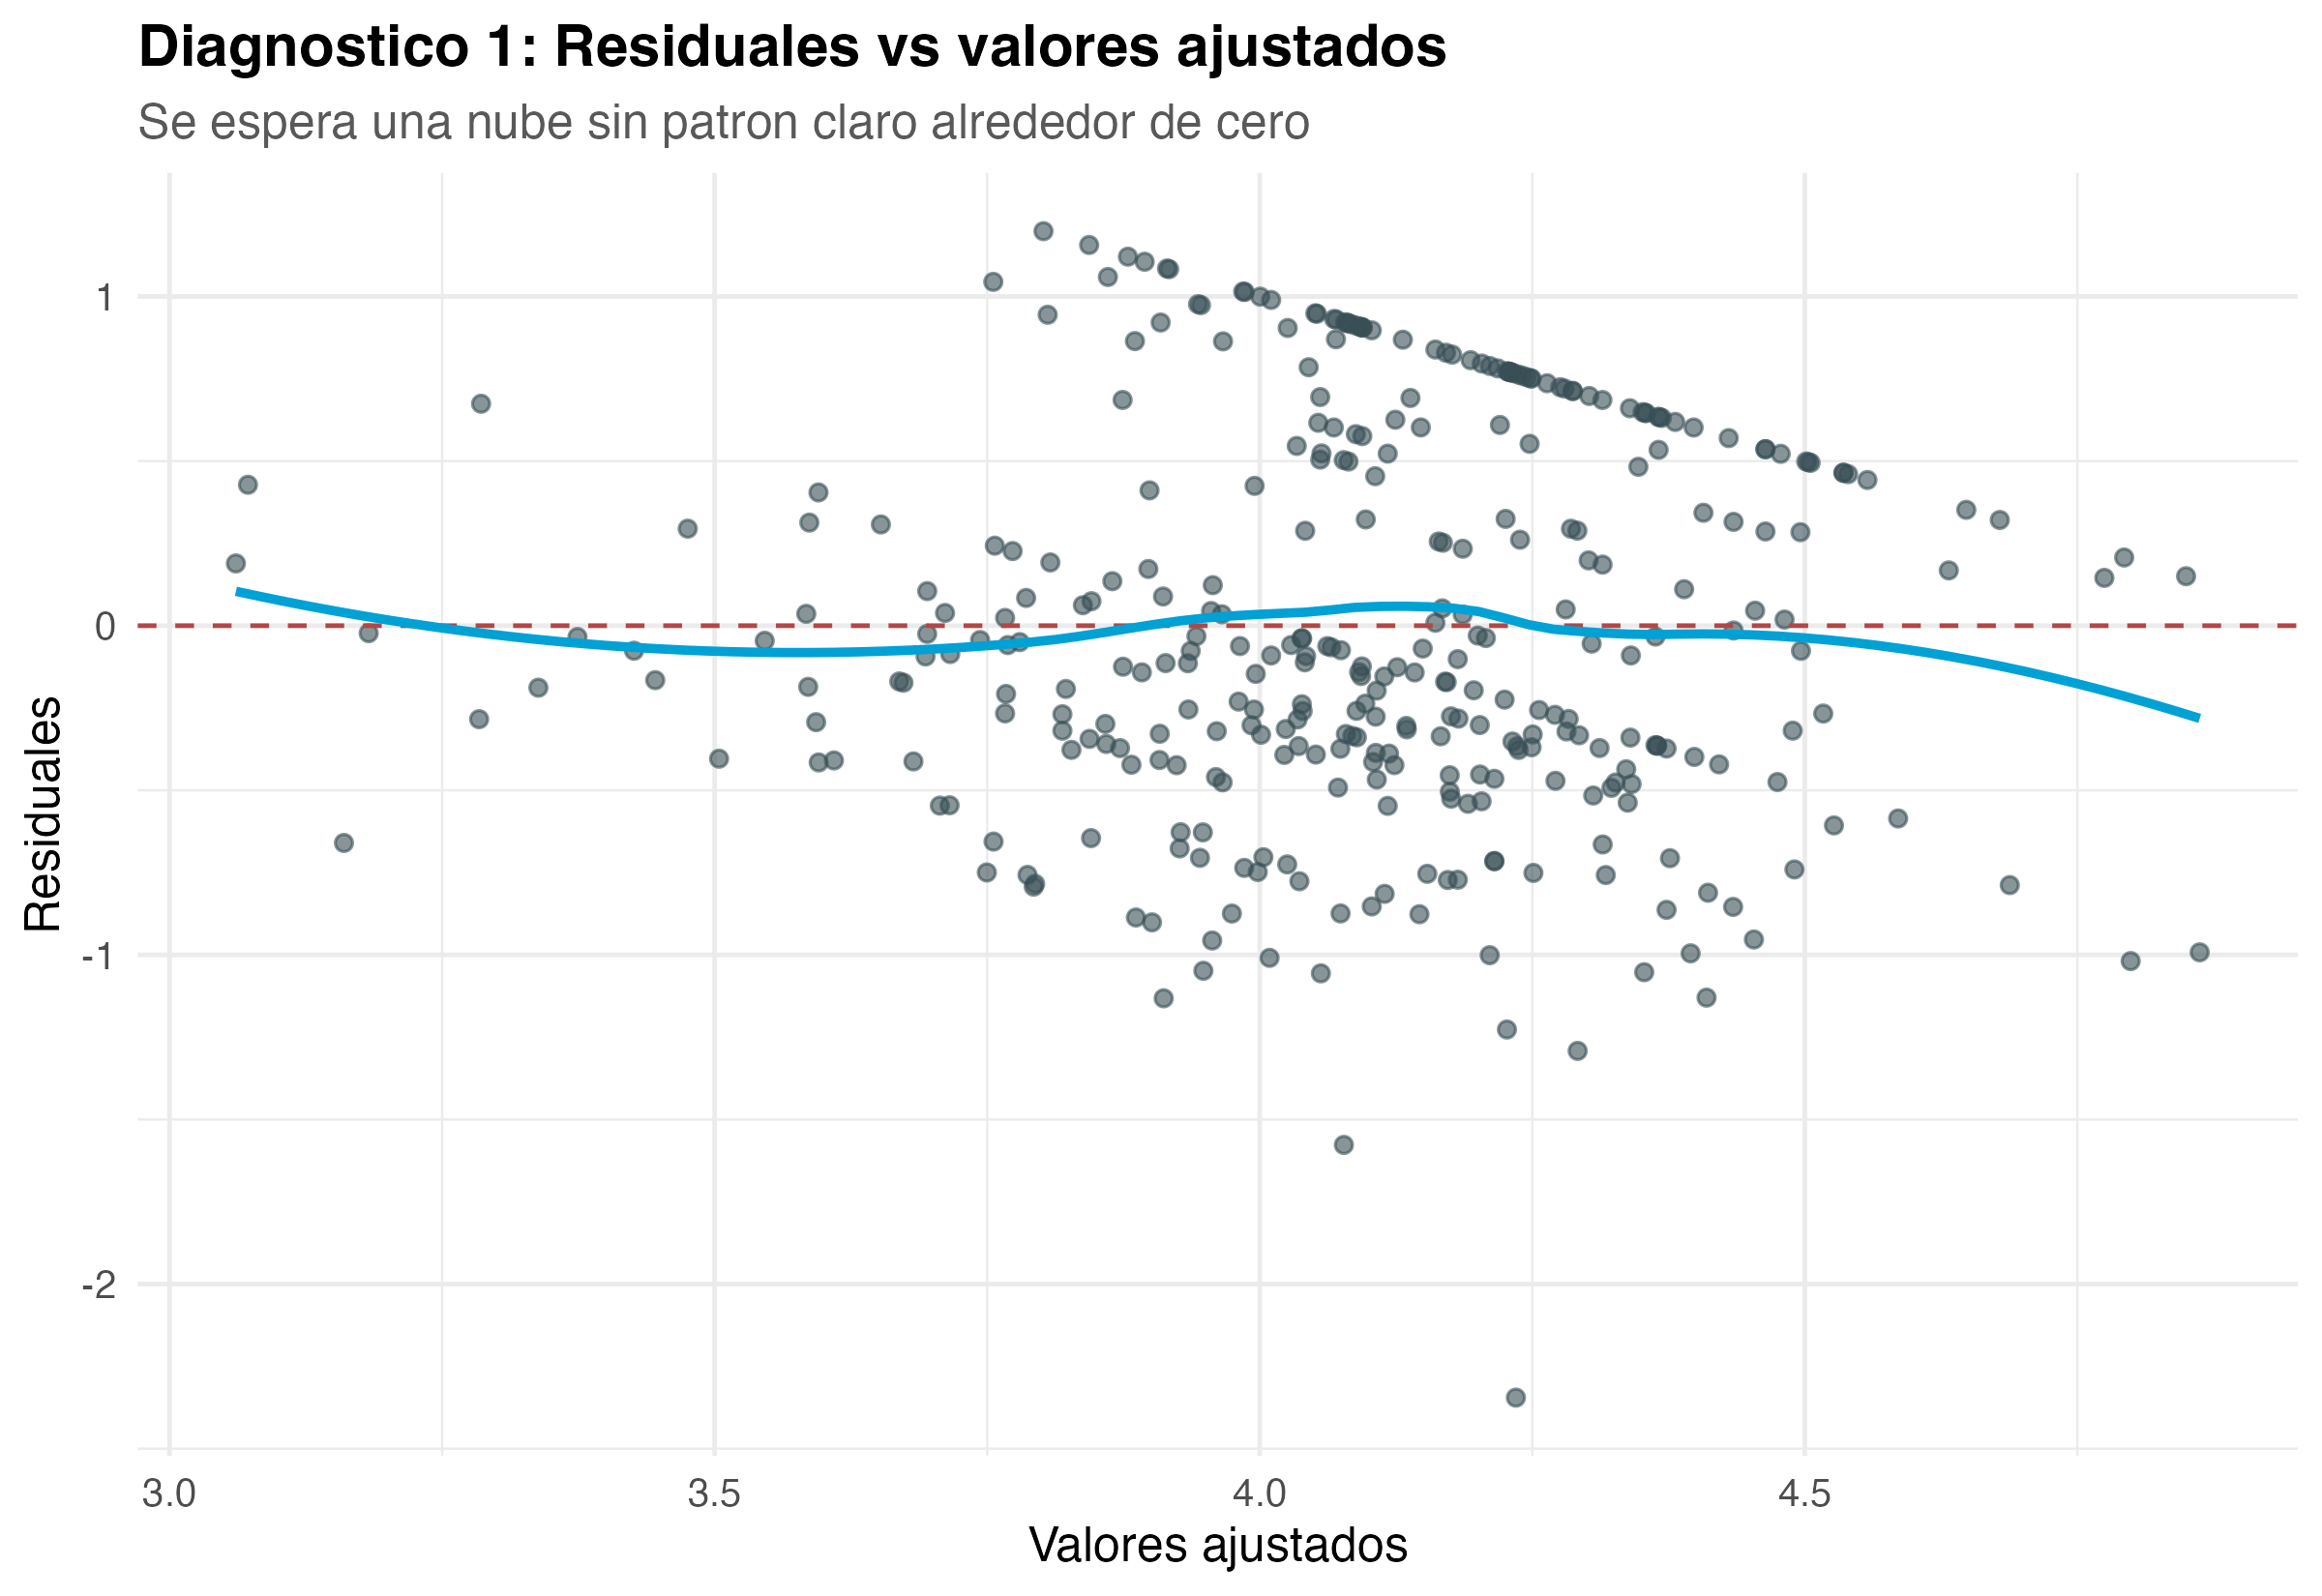
\includegraphics[width=0.75\linewidth]{figuras/diagnostico_01_residuales_vs_ajustados.png}
    \caption{Diagnóstico del modelo: residuales frente a valores ajustados}
    \label{fig:diagnostico-residuos}
\end{figure}

\begin{figure}[H]
    \centering
    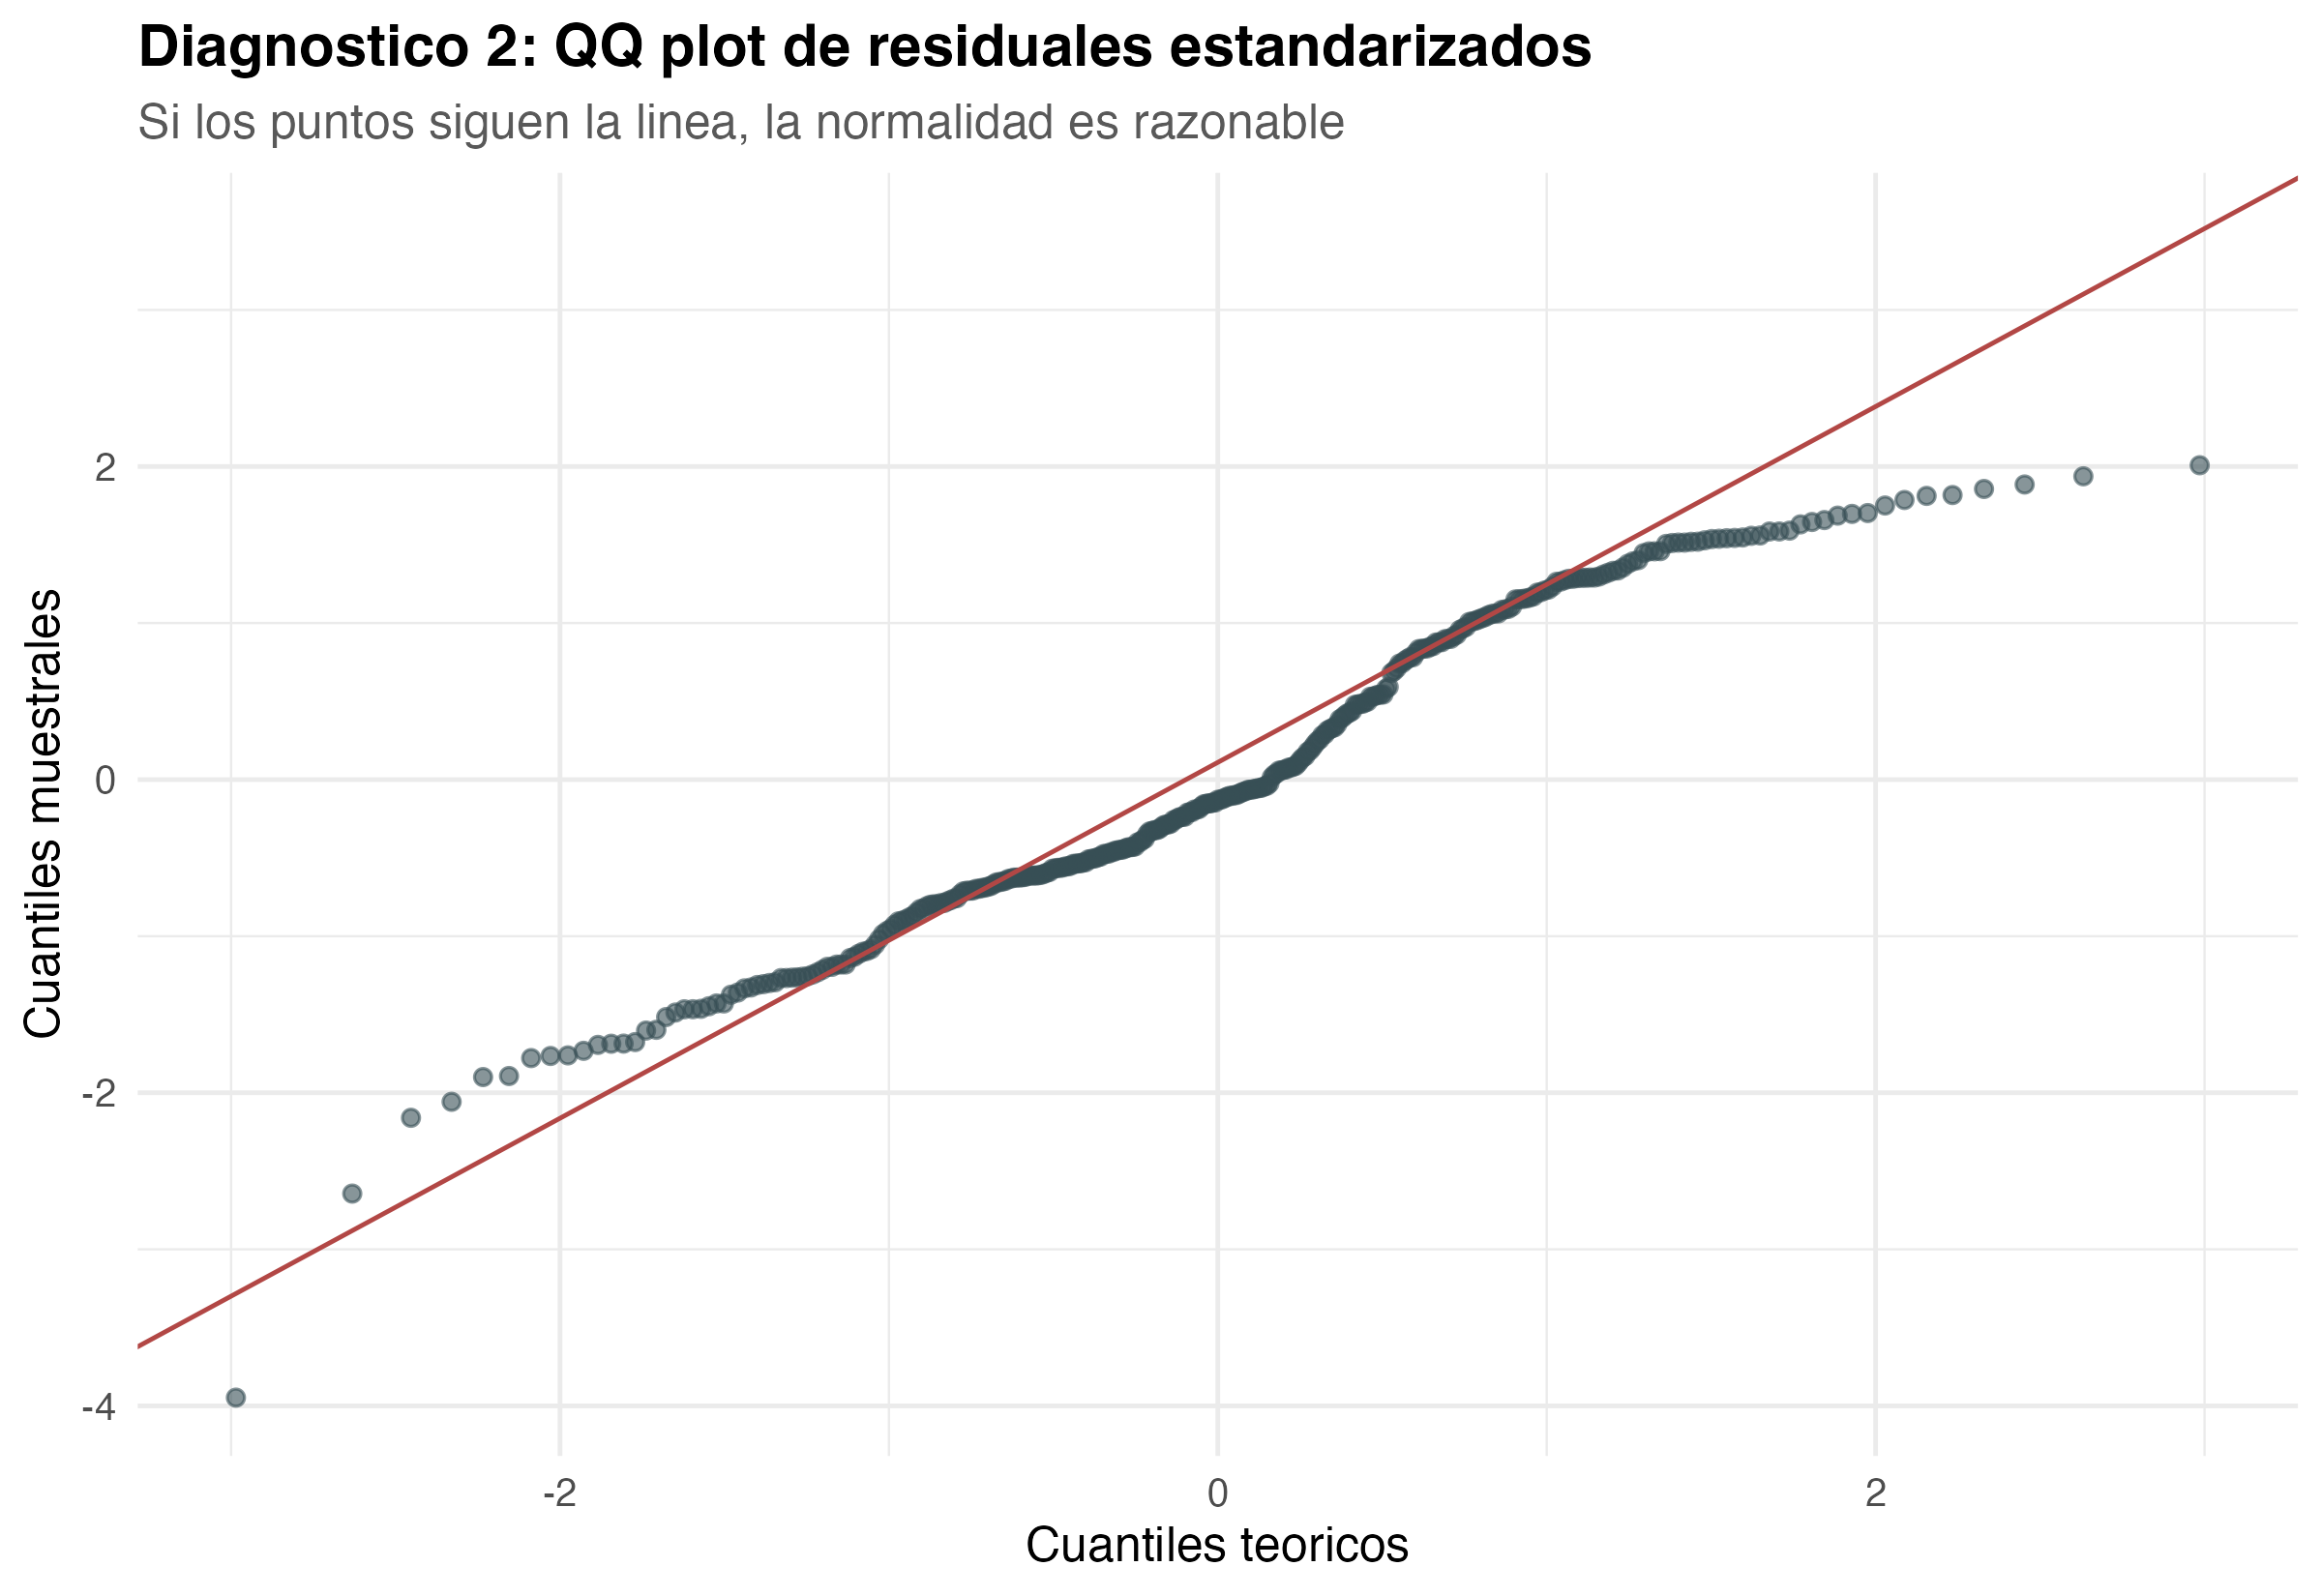
\includegraphics[width=0.75\linewidth]{figuras/diagnostico_02_qqplot_residuales.png}
    \caption{Diagnóstico del modelo: QQ plot de residuales estandarizados}
    \label{fig:diagnostico-qq}
\end{figure}

\textbf{Nivel analítico: qué significa}

\textbf{Conexión con la pregunta de investigación:} El diagnóstico no responde directamente si existe relación entre redes sociales y rendimiento, pero permite saber si el modelo usado para responder la pregunta puede interpretarse de forma razonable.

\textbf{Contraste con la literatura:} Esta ficha no se contrasta directamente con literatura teórica, porque corresponde a la validación estadística del modelo.

\textbf{Lo que NO explica este resultado:} No explica el comportamiento académico de los estudiantes. Solo revisa si el modelo presenta problemas importantes.

\textbf{Implicación para el siguiente paso:} Los resultados del modelo deben presentarse como asociaciones estadísticas y no como conclusiones causales definitivas.

\subsubsection*{Ficha 9. Modelo seleccionado}

\textbf{Nivel descriptivo: qué encontramos}

\textbf{Titular:} El rendimiento tiene varios factores.

\textbf{Nombre del hallazgo/resultado:} Modelo con horas en redes, distracción académica, horas de estudio y asistencia.

\textbf{Resumen en una oración:} El modelo fue significativo, pero explicó una parte moderada del rendimiento.

\textbf{Método o análisis que lo produjo:} Modelo de regresión lineal múltiple con interacción.

\textbf{Evidencia:} Archivos \texttt{15\_coeficientes\_modelo\_3.csv}, \texttt{16\_resumen\_modelos.txt} y \texttt{21\_metricas\_modelo\_seleccionado.csv}.

\textbf{Nivel analítico: qué significa}

\textbf{Conexión con la pregunta de investigación:} El modelo permite responder que sí existe asociación entre uso de redes sociales y rendimiento académico. Las horas en redes sociales tienen una relación negativa con el promedio, mientras que las horas de estudio y la asistencia tienen relación positiva. Además, la distracción académica también se relaciona negativamente con el rendimiento.

\textbf{Contraste con la literatura:} Esta es la ficha principal para comparar con la literatura. El resultado coincide parcialmente con estudios que señalan efectos negativos del uso excesivo de redes, pero también coincide con estudios que muestran relaciones mixtas. Esto ocurre porque el modelo muestra que las redes sociales no explican todo el rendimiento académico. El resultado más importante es que el rendimiento depende de varios factores al mismo tiempo.

\textbf{Lo que NO explica este resultado:} El modelo no explica toda la variabilidad del promedio académico. Su $R^2$ ajustado fue aproximadamente $0.172$, por lo que explica cerca del 17\% del rendimiento. Tampoco permite afirmar causalidad.

\textbf{Implicación para el siguiente paso:} En el reporte final, los resultados deben presentarse como evidencia de una relación moderada y multifactorial entre redes sociales, distracción y hábitos académicos.

\subsubsection*{Comparación explícita con la literatura}

El resultado principal del modelo coincide parcialmente con la literatura revisada. Algunos autores señalan que el uso excesivo de redes sociales puede relacionarse con menor rendimiento académico, especialmente cuando afecta la concentración o reduce el tiempo de estudio. En nuestro caso, las horas en redes sociales y la distracción académica presentaron una relación negativa con el promedio, lo cual coincide con esa interpretación.

Sin embargo, nuestros resultados también muestran que la relación no es completamente directa ni fuerte. El modelo explicó solo una parte moderada del rendimiento académico y variables como las horas de estudio y la asistencia también fueron importantes. Esto se parece a los estudios que plantean que no siempre existe una relación clara entre redes sociales y rendimiento, porque depende del contexto, del tipo de uso y de los hábitos del estudiante.

Por tanto, la principal implicación es que no podemos concluir que las redes sociales, por sí solas, expliquen el rendimiento académico. Más bien, los resultados sugieren que el problema debe entenderse como multifactorial. El uso de redes sociales importa, pero su interpretación debe hacerse junto con la distracción académica, las horas de estudio y la asistencia.
```





\subsection{Ordenamiento de los elementos de reporte}
A partir de los resultados obtenidos hasta ahora, identificamos cuáles son los aspectos más importantes para responder nuestra pregunta de investigación y cómo podrían organizarse dentro del reporte final.

\subsubsection{Elementos primarios y secundarios del reporte}
A continuación se identifican los elementos principales y secundarios del reporte.

\begin{table}[H]
\centering
\caption{Elementos primarios y secundarios del reporte}
\begin{tabular}{p{6cm} p{6cm}}
\toprule
\textbf{Elementos Primarios} & \textbf{Elementos Secundarios} \\
\midrule
Uso diario de redes sociales & Horas de sueño \\
Rendimiento académico & Horas de estudio \\
Distracción académica & Plataforma principal utilizada \\
Relación entre uso de redes y rendimiento académico & Variables demográficas \\
Influencia de la distracción sobre el rendimiento académico & Resultados específicos de otros autores \\
Resultados obtenidos en el estudio & Limitaciones de la base de datos \\
Prueba t para comparar grupos de uso & Uso nocturno de redes sociales \\
ANOVA para comparar categorías de uso de redes & Comparaciones descriptivas por plataforma \\
Prueba de Kruskal-Wallis como alternativa no paramétrica & Variables de bienestar emocional \\
Correlaciones de Pearson y Spearman & Tamaños de muestra por grupo \\
Modelo seleccionado de rendimiento académico & Figuras exploratorias de la Bitácora 2 \\
Diagnósticos del modelo seleccionado & Advertencias sobre asociación y no causalidad \\
\bottomrule
\end{tabular}
\end{table}

\subsubsection{Orden propuesto para el artículo final}
Con base a los elementos anteriores se propone el siguiente orden para la redacción del artículo final.

\begin{table}[H]
\centering
\caption{Orden propuesto para el artículo final}
\begin{tabular}{p{3cm} p{9cm}}
\toprule
\textbf{Sección} & \textbf{Temas a tratar} \\
\midrule
Introducción & Uso de redes sociales en estudiantes universitarios (Primario) \\
Introducción & Relación entre redes sociales y rendimiento académico (Primario) \\
Introducción & Resultados encontrados por León Luyo (Secundario) \\
Introducción & Resultados encontrados por Rodelo Moreno y Lizárraga Reyes (Secundario) \\
Introducción & Papel potencial de la distracción académica (Primario) \\
Introducción & Importancia de estudiar la relación como asociación y no como causalidad (Primario) \\
\midrule
Metodología & Descripción de la base de datos (Primario) \\
Metodología & Variables seleccionadas (Primario) \\
Metodología & Construcción de grupos de uso de redes sociales (Primario) \\
Metodología & ANOVA y prueba t (Primario) \\
Metodología & Correlaciones de Pearson y Spearman (Primario) \\
Metodología & Prueba de Kruskal-Wallis como respaldo no paramétrico (Primario) \\
Metodología & Ajuste del modelo seleccionado con horas en redes, distracción académica, horas de estudio y asistencia (Primario) \\
Metodología & Diagnósticos del modelo seleccionado: residuos, normalidad, valores influyentes y multicolinealidad (Primario) \\
Metodología & Análisis fallido basado en la clasificación por red social principal (Secundario) \\
\midrule
Resultados & Relación entre uso de redes sociales y promedio académico (Primario) \\
Resultados & Diferencias de promedio entre grupos de uso de redes sociales (Primario) \\
Resultados & Resultado de la prueba t entre bajo/moderado uso y alto uso (Primario) \\
Resultados & Resultado del ANOVA entre categorías de uso de redes (Primario) \\
Resultados & Resultado de Kruskal-Wallis como comparación no paramétrica (Primario) \\
Resultados & Correlaciones entre promedio académico, horas en redes, horas de estudio, asistencia y distracción académica (Primario) \\
Resultados & Influencia de la distracción académica (Primario) \\
Resultados & Resultados del modelo seleccionado (Primario) \\
Resultados & Diagnósticos del modelo seleccionado (Primario) \\
Resultados & Comparación con estudios previos (Secundario) \\
Resultados & Influencia de horas de estudio y sueño (Secundario) \\
\midrule
Discusión & Interpretación general de los resultados obtenidos (Primario) \\
Discusión & Comparación entre lo esperado según la literatura y lo encontrado en la muestra (Primario) \\
Discusión & Alcances y limitaciones del análisis (Primario) \\
Discusión & Posibles variables no observadas que podrían influir en el rendimiento académico (Secundario) \\
\bottomrule
\end{tabular}
\end{table}

\subsection{La imagen que cuenta la historia}

\begin{figure}[H]
    \centering
    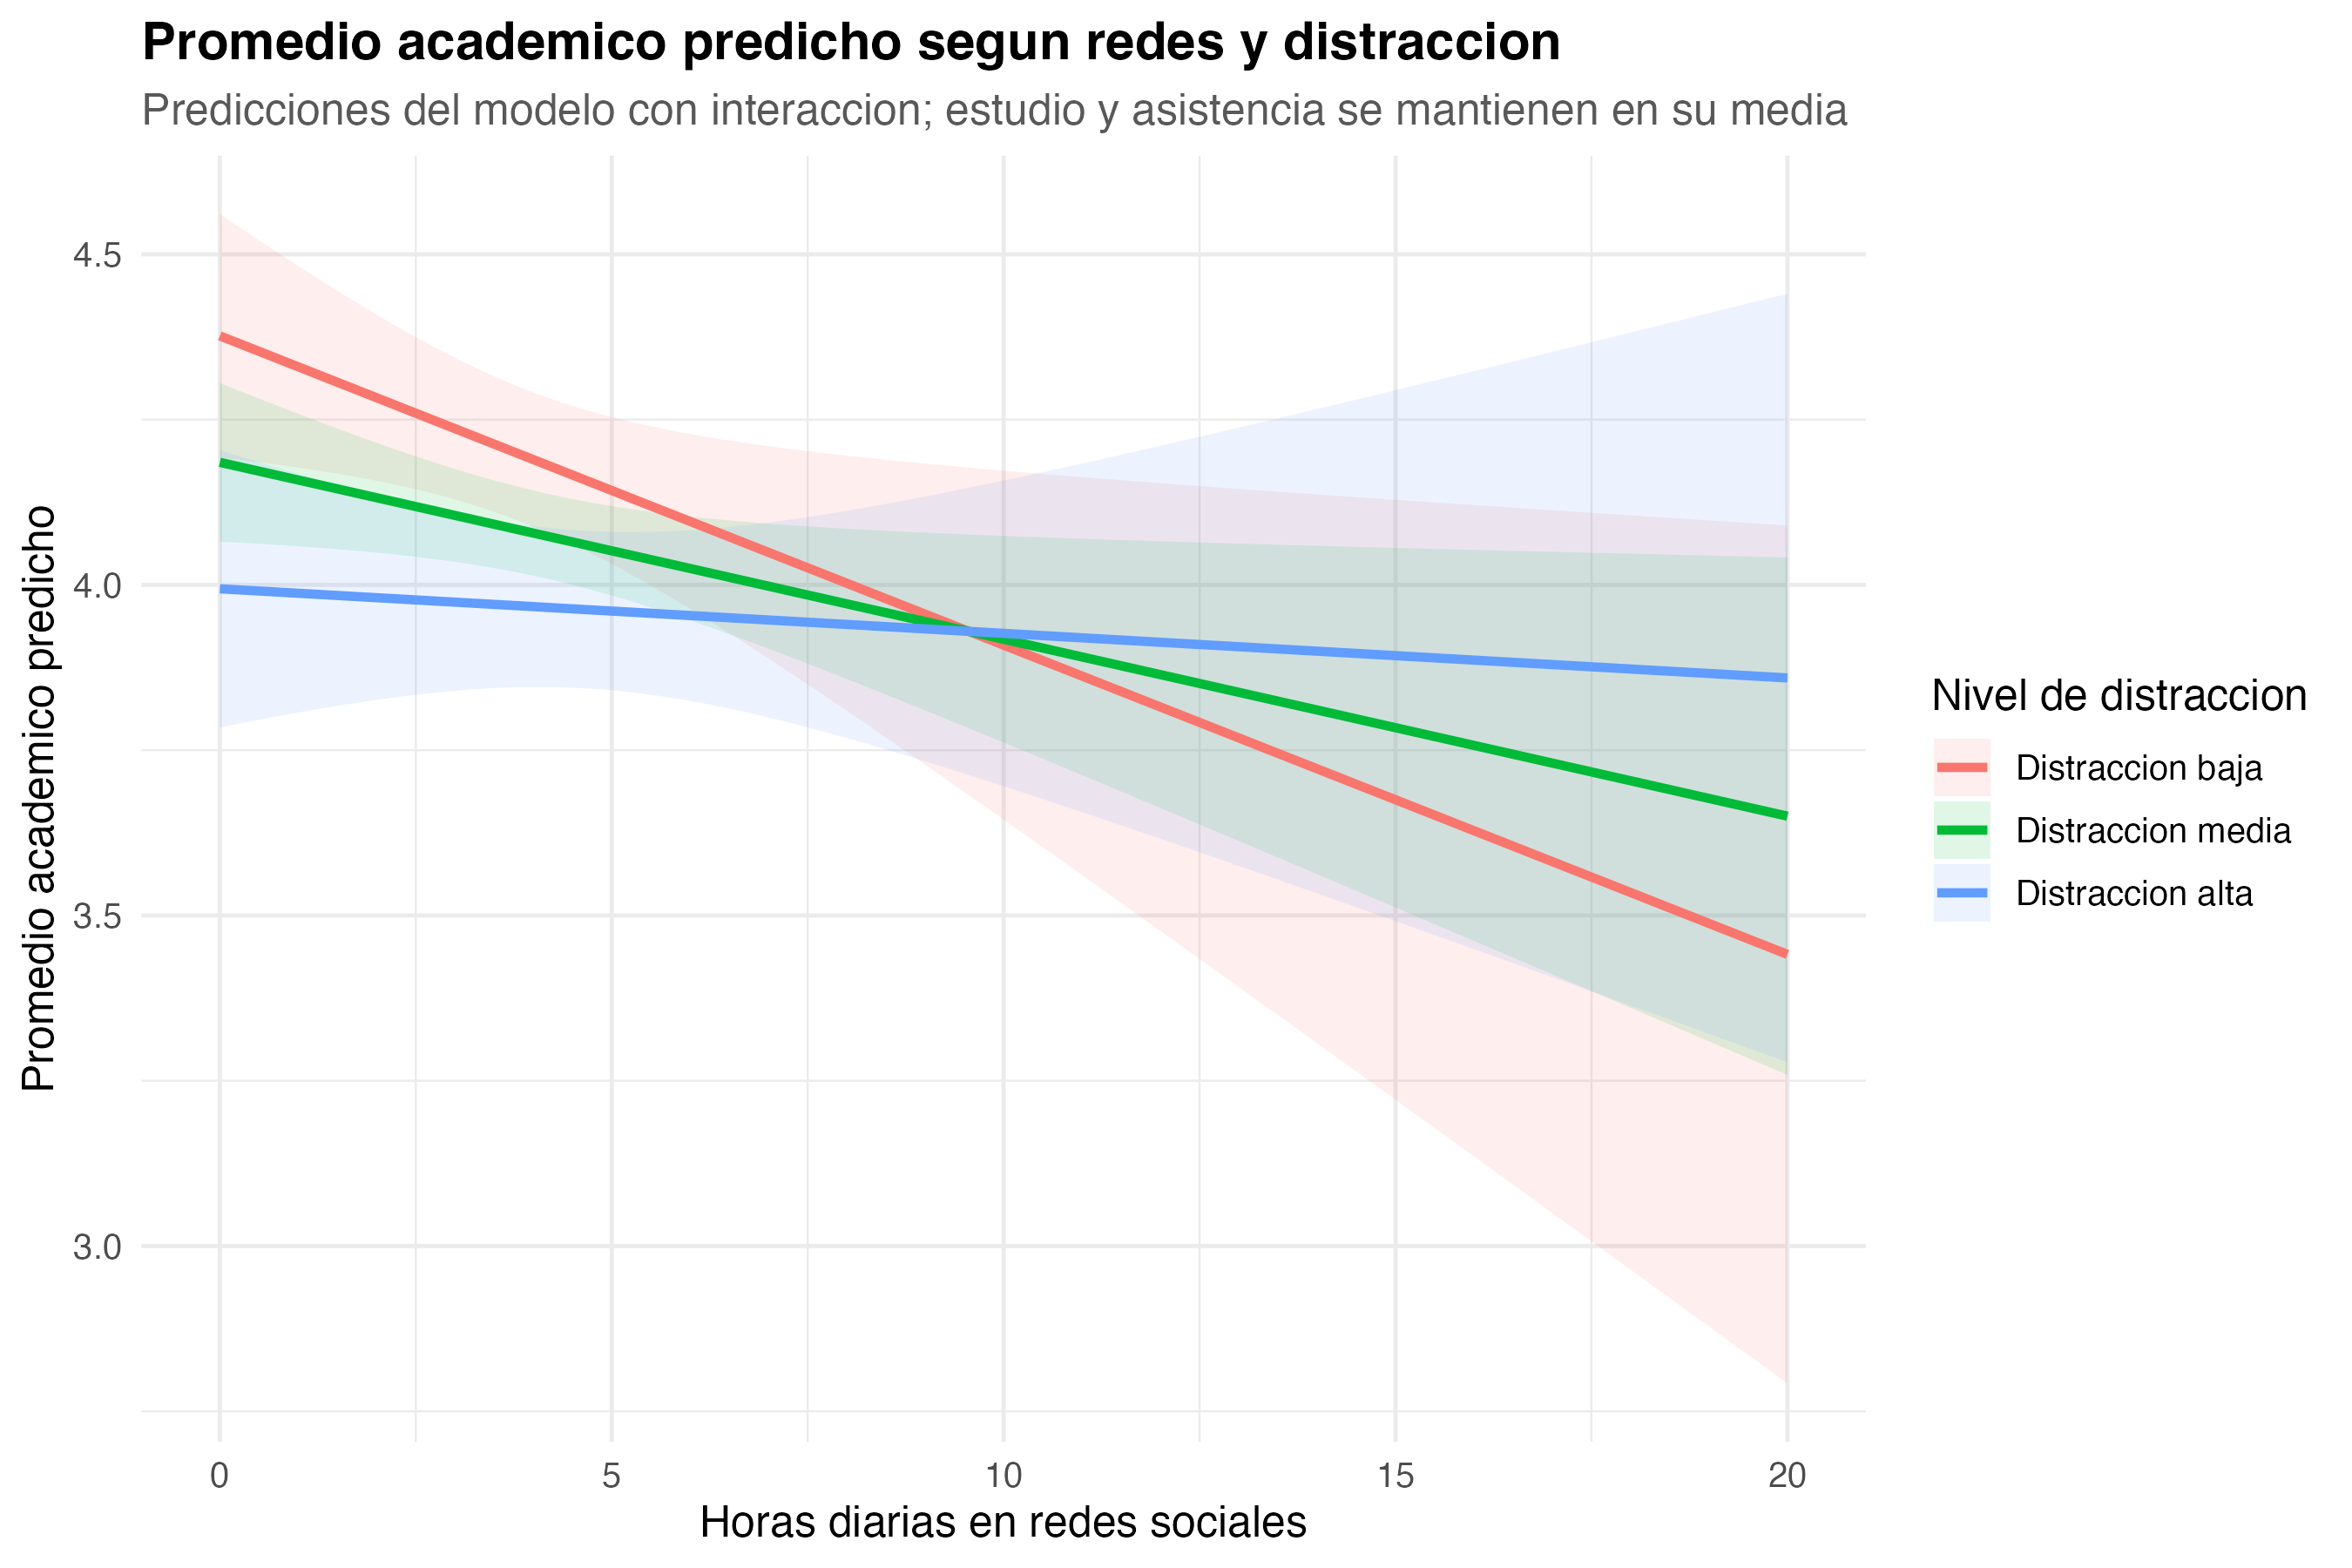
\includegraphics[width=0.85\textwidth]{figuras/figura_06_predicciones_modelo_interaccion.png}
    \caption{Promedio académico predicho según horas en redes sociales y distracción académica}
    \label{fig:predicciones-modelo-interaccion}
\end{figure}

De todos los gráficos generados en esta bitácora, escogimos como imagen principal la Figura \ref{fig:predicciones-modelo-interaccion}, que muestra las predicciones del modelo con interacción. Este gráfico fue seleccionado porque resume la idea central de esta etapa del proyecto: el rendimiento académico no debe analizarse únicamente a partir de las horas en redes sociales, sino también considerando otras variables como la distracción académica, las horas de estudio y la asistencia. A diferencia de los gráficos exploratorios de la Bitácora 2, esta imagen ya incorpora el modelo estadístico y permite observar el comportamiento esperado del promedio académico según distintos niveles de uso de redes y distracción.

Este gráfico es más fuerte que un boxplot o una dispersión simple porque no solo muestra puntos observados, sino una tendencia estimada por el modelo. Al observarlo, una persona podría tomar la decisión de no enfocarse únicamente en reducir el tiempo total en redes sociales, sino también en mejorar la forma en que los estudiantes manejan la distracción durante sus actividades académicas. La imagen ayuda a entender que dos estudiantes pueden usar redes sociales durante una cantidad similar de horas, pero no necesariamente tener el mismo rendimiento si sus hábitos de estudio y niveles de distracción son diferentes.

Desde la Bitácora 2, nuestra comprensión del problema cambió bastante. Al inicio pensábamos que la relación podía explicarse principalmente por el tiempo de uso de redes sociales. Sin embargo, los resultados exploratorios y la modelación muestran que el fenómeno es más complejo. Las horas en redes sí parecen tener una relación con el promedio, pero no explican todo el rendimiento académico. También importan variables académicas como las horas de estudio y la asistencia.

Si este gráfico fuera la portada del artículo, contaría la historia de un problema que no puede reducirse a la idea de que ``más redes sociales significan peores notas''. Más bien, mostraría que el rendimiento académico depende de varios factores que actúan al mismo tiempo. La historia principal sería que el uso de redes sociales debe analizarse junto con el contexto académico del estudiante. Por eso, esta imagen representa bien el avance de la Bitácora 3: pasamos de describir patrones a construir una explicación estadística más completa.

\section{Arco narrativo del proyecto}

El modelo reveló que el uso de redes sociales se relaciona negativamente con el promedio académico, pero que las horas de estudio y la asistencia también tienen un papel importante, lo que significa que el rendimiento académico debe entenderse como un fenómeno multifactorial y no como consecuencia directa de una sola variable.

\section{Parte de escritura}
En las bitácoras anteriores realizamos una revisión bibliográfica sobre la relación entre el uso de redes sociales y el rendimiento académico, además de un análisis exploratorio de la base de datos utilizada en el proyecto. En esta sección buscamos integrar ambas perspectivas para construir una única narrativa sobre el problema estudiado, relacionando lo que han encontrado otros autores con los patrones observados en nuestros propios datos.

\subsection{Redes sociales y rendimiento académico}

El uso de redes sociales se ha convertido en una actividad habitual para la mayoría de estudiantes universitarios. Plataformas como Instagram, TikTok, YouTube o WhatsApp forman parte de su día a día y se utilizan tanto para comunicarse como para entretenerse, informarse o incluso realizar actividades académicas. Debido a esta presencia constante, se ha tratado de determinar si existe alguna relación entre el tiempo dedicado a estas plataformas y el rendimiento académico.
\\

Sin embargo, las conclusiones encontradas en la literatura no son siempre las mismas. Algunos estudios sostienen que un uso elevado de redes sociales puede relacionarse con peores resultados académicos. Entre las explicaciones más frecuentes aparecen la reducción del tiempo disponible para estudiar, las interrupciones durante el estudio o la tendencia a posponer tareas importantes debido al uso frecuente de estas plataformas.
\\

Por otro lado, también encontramos investigaciones que muestran una visión más matizada. León Luyo et al. (2023), por ejemplo, no encuentran una relación significativa entre ambas variables, mientras que Rodelo Moreno y Lizárraga Reyes (2018) señalan que las redes sociales incluso pueden tener efectos positivos cuando se utilizan con fines académicos. Estos resultados sugieren que el tiempo de uso, por sí solo, podría no ser suficiente para explicar las diferencias observadas en el rendimiento académico.
\\

Esta falta de consenso fue una de las principales razones por las que decidimos abordar este tema. Más que partir de la idea de que las redes sociales son beneficiosas o perjudiciales, nos interesaba analizar qué ocurría en nuestra muestra y comprobar si los patrones observados coincidían con alguno de los resultados encontrados en la literatura. Además, nos parecía interesante identificar qué otras variables podían estar influyendo en esta relación.

\subsection{Qué muestran nuestros datos}

Una vez revisada la literatura, comenzamos a explorar la información contenida en nuestra base de datos. El conjunto de datos está formado por estudiantes universitarios e incluye variables relacionadas con el uso de redes sociales, rendimiento académico, hábitos de estudio, horas de sueño y nivel de distracción, entre otras.
\\

Uno de los primeros aspectos que analizamos fue el tiempo de uso diario de redes sociales. Los resultados muestran que se trata de una actividad muy frecuente dentro de la muestra. La mayoría de estudiantes dedica varias horas al día a estas plataformas, aunque existen diferencias importantes entre unos estudiantes y otros. Para esta parte se utilizó la distribución de las horas de uso de redes sociales y la comparación por categorías de uso. Esto permitió observar que el tiempo en redes no se distribuye igual entre todos los estudiantes y que existen grupos con bajo, medio y alto uso diario.
\\

Esta distribución coincide con lo descrito por muchos de los estudios revisados, donde se señala que las redes sociales forman parte de la rutina diaria de la mayoría de estudiantes universitarios. Sin embargo, saber cuántas horas utilizan estas plataformas no permite responder directamente a nuestra pregunta de investigación.
\\

Para profundizar en esta cuestión analizamos conjuntamente las horas de uso de redes sociales y el promedio académico de los estudiantes.

\begin{figure}[H]
    \centering
    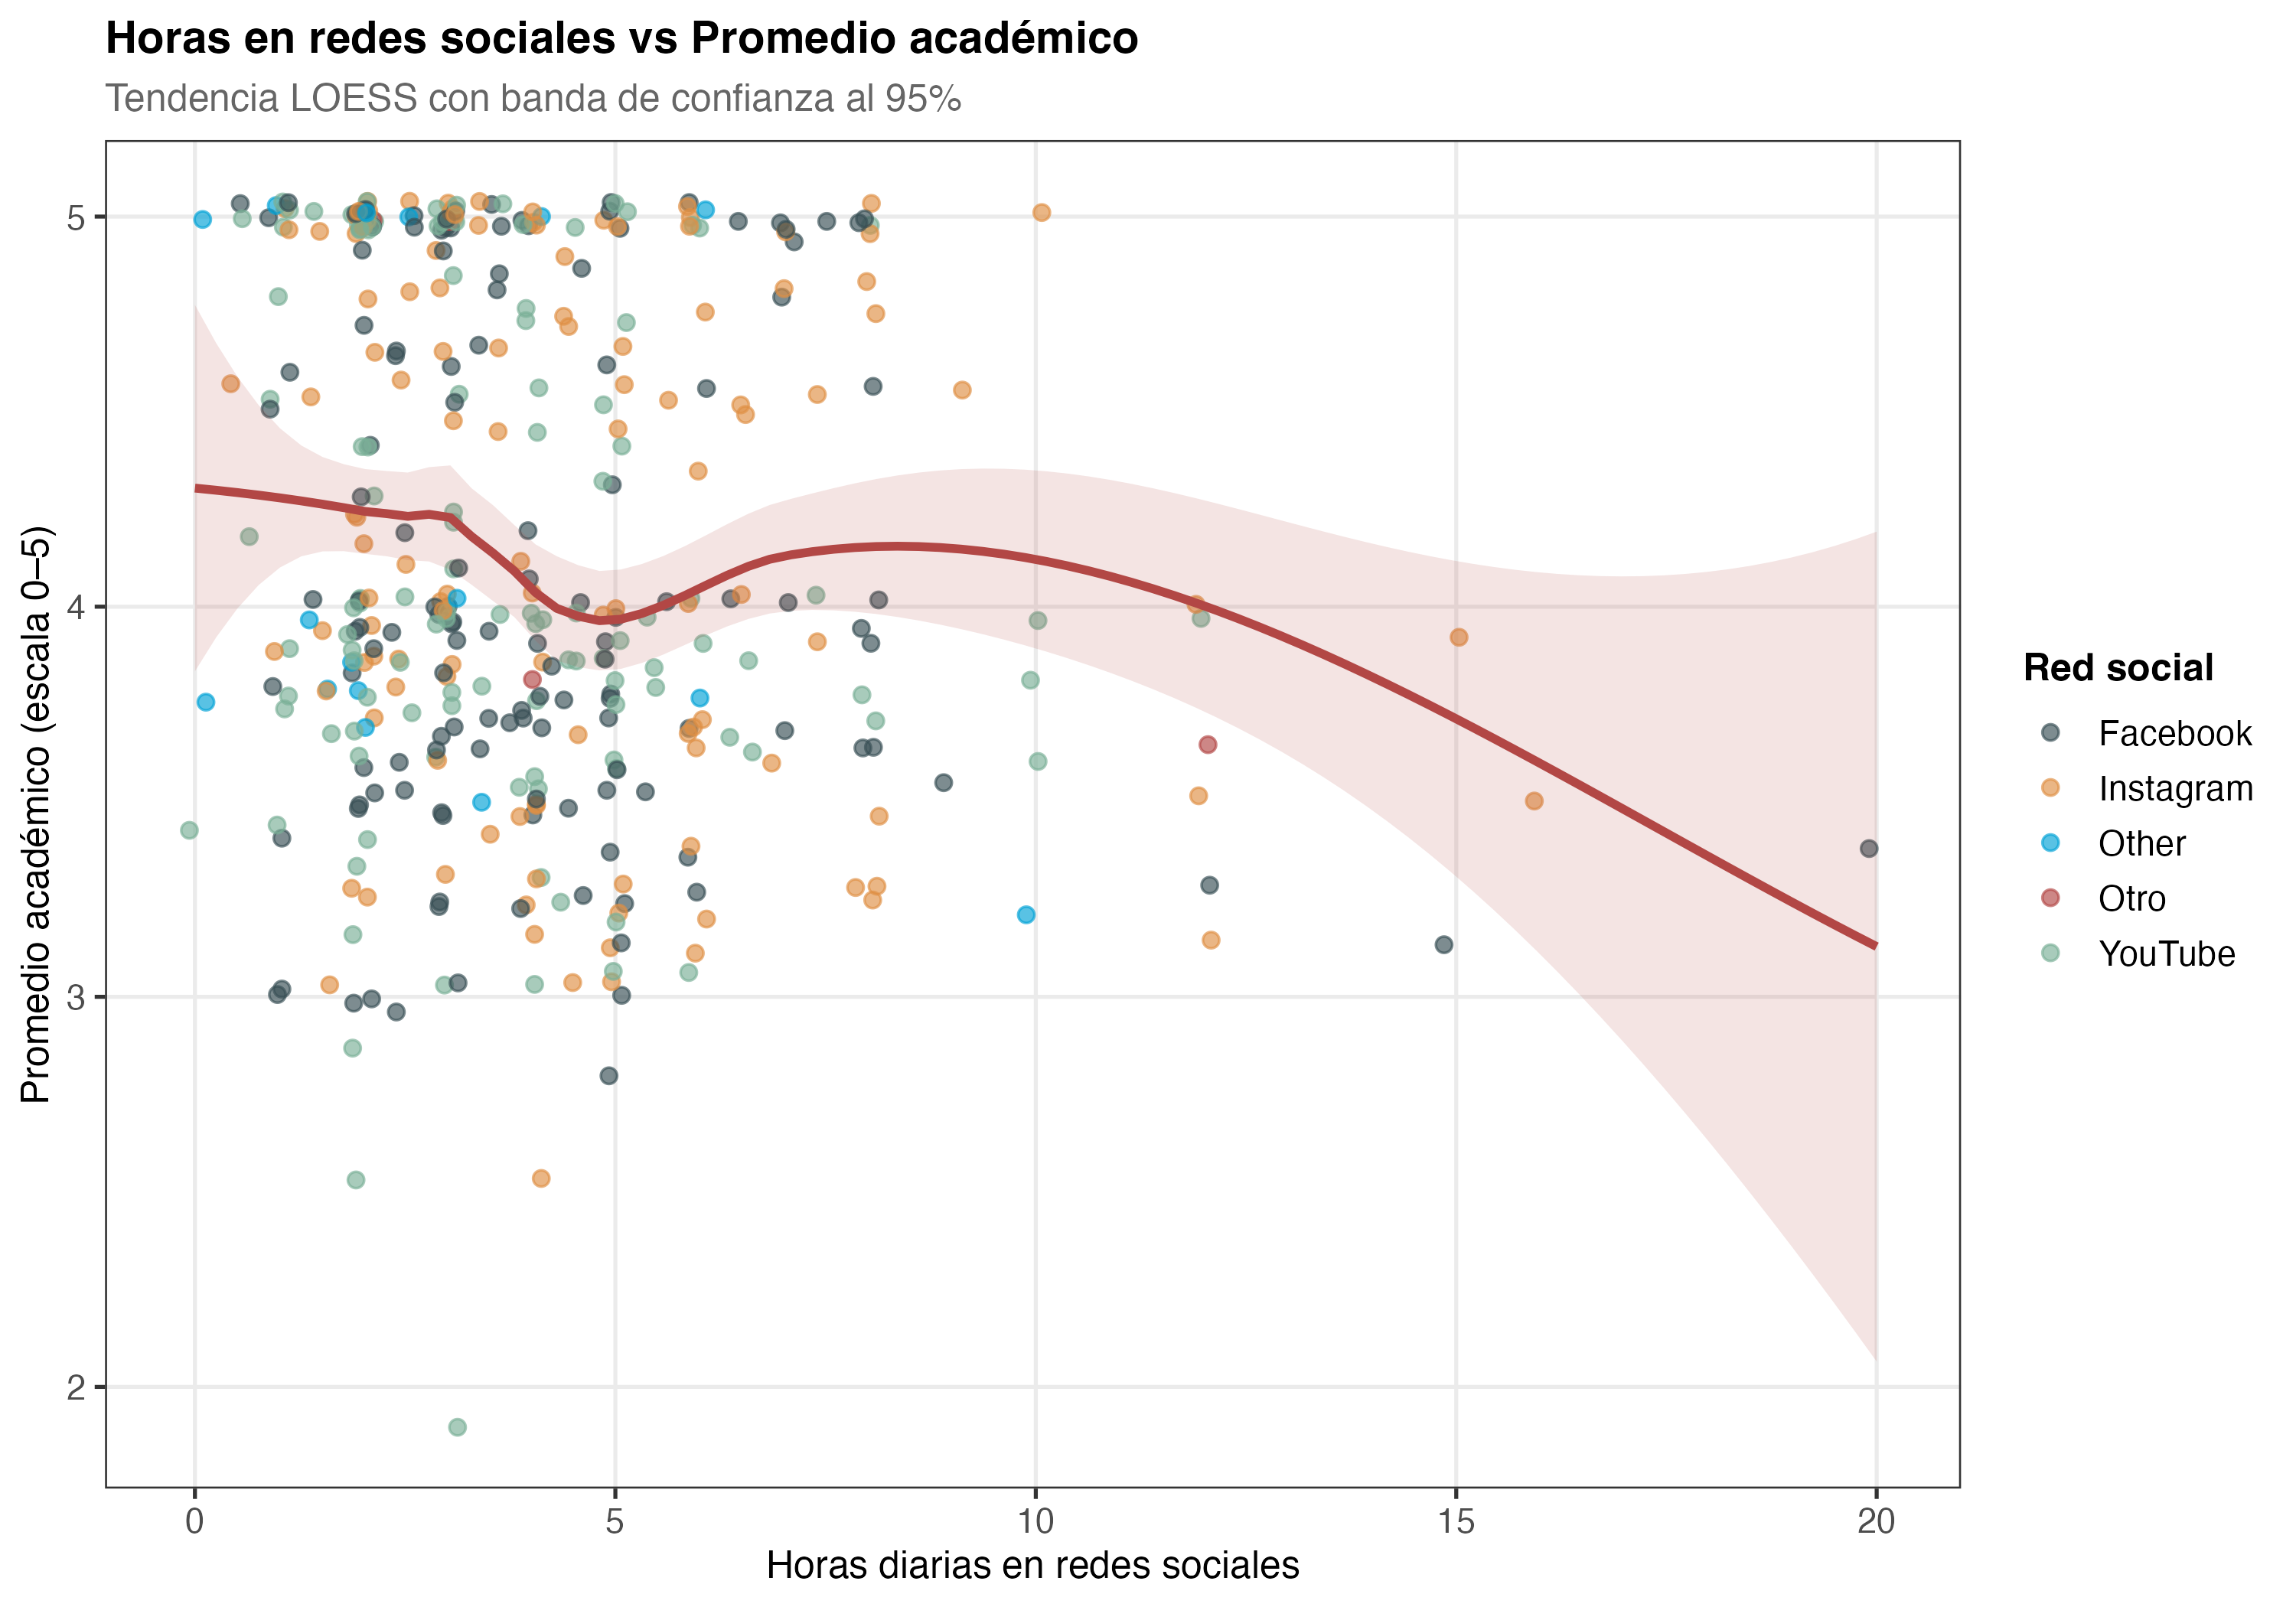
\includegraphics[width=0.7\linewidth]{figuras/grafico_1_horas_redes_vs_promedio.png}
    \caption{Asociación entre el tiempo diario en redes sociales y el promedio académico en estudiantes universitarios}
    \label{fig:redesvsprom}
\end{figure}

Este fue uno de los resultados que más nos llamó la atención durante el análisis exploratorio. Inicialmente esperábamos encontrar una relación más evidente entre ambas variables. Sin embargo, los datos mostraron una situación bastante más compleja. Aunque algunos estudiantes con muchas horas de uso presentan promedios relativamente bajos, también encontramos estudiantes con niveles de uso similares que mantienen buenos resultados académicos.
\\

Si el tiempo de uso fuese el único factor importante, esperaríamos observar una tendencia mucho más clara. No obstante, los datos muestran una gran variabilidad entre estudiantes. Personas con hábitos parecidos respecto al uso de redes sociales pueden presentar desempeños académicos muy diferentes.
\\

A raíz de estas observaciones empezamos a plantearnos si otras variables de la base de datos podían estar influyendo en la relación entre redes sociales y rendimiento académico. Más que proporcionarnos una respuesta definitiva, el análisis exploratorio nos ayudó a formular nuevas preguntas y a identificar aspectos que merecían una atención más detallada en las siguientes etapas del proyecto.



\subsection{La distracción académica como posible explicación}

Conforme analizábamos los datos, vimos que las horas de uso de redes sociales no parecían suficientes para explicar las diferencias observadas en el rendimiento académico. Aunque algunos estudiantes con muchas horas de uso presentaban promedios académicos bajos, también encontramos estudiantes con niveles de uso similares que mantenían buenos resultados. Este fue uno de los aspectos que más nos llamó la atención durante el análisis exploratorio.
\\

Por ello empezamos a fijarnos en otras variables que inicialmente no habíamos considerado tan importantes. Entre ellas, la variable de distracción académica resultó especialmente interesante. Mientras que las horas de uso indican cuánto tiempo pasa un estudiante utilizando redes sociales, la distracción académica intenta reflejar hasta qué punto ese uso interfiere en actividades relacionadas con el estudio, la realización de tareas o la preparación de exámenes.

\begin{figure}[H]
    \centering
    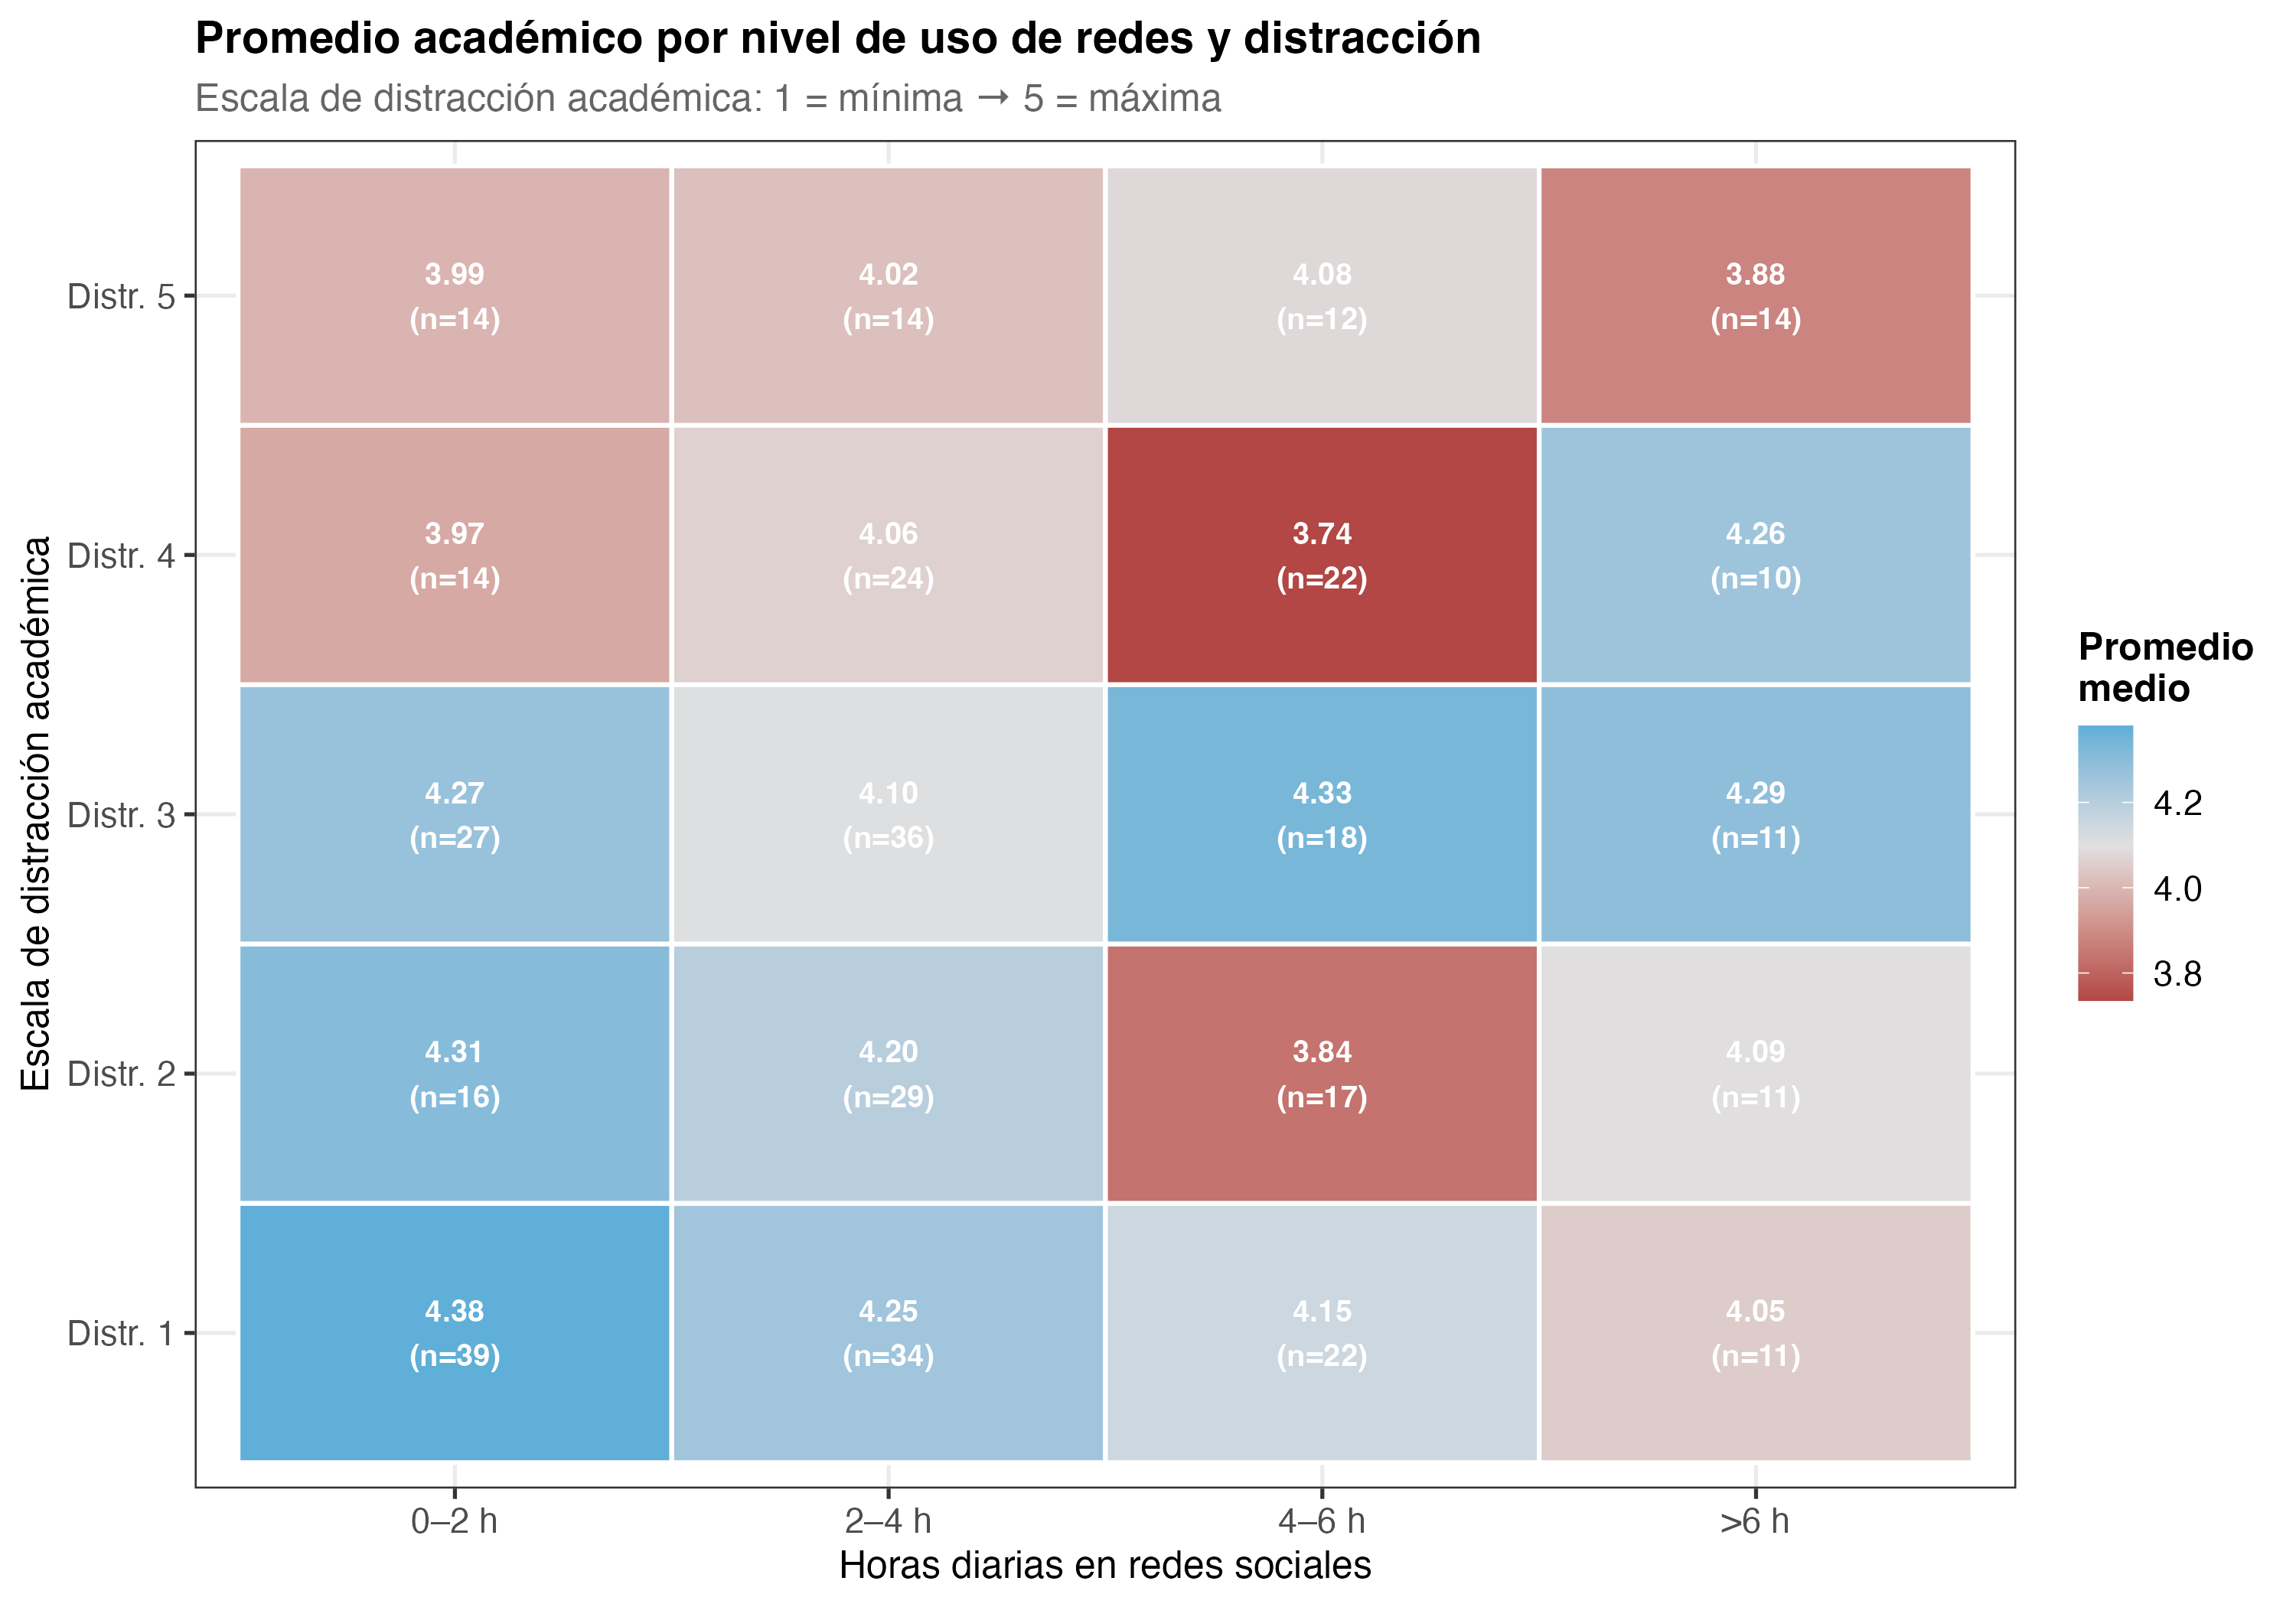
\includegraphics[width=0.7\linewidth]{figuras/grafico_5_heatmap_redes_distraccion_promedio.png}
    \caption{Promedio académico medio según nivel de uso de redes sociales y grado de distracción durante actividades académicas}
    \label{fig:heatmap}
\end{figure}

En los gráficos observamos que los estudiantes con niveles bajos de distracción suelen presentar promedios académicos más altos que aquellos que se consideran más distraídos. Del mismo modo, los niveles elevados de distracción parecen asociarse con peores resultados académicos. Aunque estas observaciones todavía deben ser contrastadas mediante pruebas estadísticas, fueron una de las tendencias más claras que encontramos durante el análisis descriptivo.
\\

Esta idea también aparece en algunos de los trabajos revisados. Ogunbiyi (2024) señala que las redes sociales pueden aportar beneficios académicos cuando se utilizan de forma adecuada, pero que un uso excesivo puede afectar negativamente a la concentración. De forma parecida, Aljemely (2020) plantea que la adicción a redes sociales y teléfonos inteligentes puede terminar influyendo en el rendimiento académico a través de mecanismos relacionados con la atención y la concentración.
\\

Lo que observamos en nuestra base de datos parece ir en esa misma dirección. Más que las horas de uso consideradas de forma aislada, podría ser la capacidad de las redes sociales para distraer al estudiante uno de los factores que mejor ayude a explicar las diferencias observadas en el rendimiento académico. Esto permitiría entender por qué algunos estudiantes mantienen buenas calificaciones a pesar de dedicar varias horas al día a las redes sociales, mientras que otros presentan más dificultades académicas con niveles de uso similares.
\\

Después de observar estos resultados, consideramos que la distracción académica debía ocupar un papel más importante dentro del proyecto. Por ello decidimos incorporarla como una de las variables principales en los análisis posteriores y estudiar no solo su relación individual con el rendimiento académico, sino también cómo interactúa con el uso de redes sociales.

\subsection{Comparación con la literatura}

Después del análisis exploratorio quisimos comparar nuestros resultados con los estudios revisados al inicio del proyecto. Aunque todos ellos analizan la relación entre redes sociales y rendimiento académico, las conclusiones obtenidas no siempre son las mismas.
\\
Por un lado, algunos trabajos encuentran relaciones débiles o incluso inexistentes entre ambas variables. Este es el caso de León Luyo et al. (2023), quienes concluyen que no existe una relación significativa entre el uso de redes sociales y el rendimiento académico de los estudiantes analizados. A pesar de ello, los autores también señalan que algunos estudiantes perciben beneficios derivados del uso de estas plataformas, especialmente cuando se utilizan con fines educativos.
\\

Lo que hemos observado en nuestra muestra encaja bastante bien con esta idea. Durante el análisis exploratorio no encontramos una relación simple ni claramente lineal entre las horas de uso de redes sociales y el promedio académico. La presencia de estudiantes con muchas horas de uso y buenos resultados académicos sugiere que el tiempo dedicado a estas plataformas no determina por sí solo el desempeño académico.
\\
Sin embargo, otros autores sí encuentran evidencias de efectos negativos asociados al uso intensivo de redes sociales. Aljemely (2020) relaciona la adicción tecnológica con una disminución del rendimiento académico, mientras que Ogunbiyi (2024) destaca que un uso excesivo puede afectar a la concentración y dificultar el aprendizaje. Este planteamiento también ayuda a interpretar algunos de los patrones que encontramos en nuestros datos, especialmente cuando analizamos la variable de distracción académica.
\\

También encontramos estudios con resultados más específicos. Rodelo Moreno y Lizárraga Reyes (2018) señalan que las redes sociales pueden incluso presentar asociaciones positivas con el rendimiento académico cuando se utilizan para compartir información, resolver dudas o acceder a contenidos educativos. Esta posibilidad nos parece especialmente interesante porque podría explicar por qué distintos estudios llegan a conclusiones tan diferentes. No todos los estudiantes utilizan las redes sociales de la misma forma y, por tanto, tampoco es razonable esperar que sus efectos sean exactamente iguales.
\\

Después de revisar la literatura y analizar nuestros datos, la principal conclusión a la que hemos llegado es que la relación entre redes sociales y rendimiento académico parece bastante más compleja de lo que pensábamos al inicio del proyecto. Los resultados no apuntan a una explicación única y probablemente intervienen varios factores al mismo tiempo, como la distracción, los hábitos de estudio, la organización del tiempo o el uso académico que cada estudiante hace de estas plataformas.
\\

Precisamente por ello, las pruebas estadísticas seleccionadas constituyen una herramienta fundamental para determinar si las tendencias observadas durante el análisis descriptivo corresponden a relaciones estadísticamente significativas o si pueden explicarse por la variabilidad propia de los datos.\\

\subsection{Discusión preliminar}

A partir de los análisis realizados, podemos decir que la relación entre el uso de redes sociales y el rendimiento académico existe, pero no es una relación simple. Al inicio del proyecto pensábamos que el tiempo diario en redes sociales podía explicar de forma clara las diferencias en el promedio académico. Sin embargo, los resultados muestran que esta explicación es incompleta. Hay estudiantes que usan redes sociales durante varias horas al día y aun así mantienen buenos promedios, mientras que otros con niveles parecidos de uso presentan resultados más bajos.
\\

El modelo ajustado ayuda a entender mejor esta situación. Las horas en redes sociales presentan una relación negativa con el promedio académico. Esto significa que, dentro de la muestra, los estudiantes que pasan más tiempo en redes tienden a tener promedios ligeramente menores. No obstante, esta relación no debe interpretarse como causalidad. Es decir, no podemos afirmar que las redes sociales causen directamente una disminución en el rendimiento académico, sino que ambas variables aparecen asociadas en los datos.
\\

También se observó que la distracción académica tiene una relación negativa con el promedio. Este resultado es importante porque apoya una de las ideas principales que surgió durante el análisis exploratorio: no solo importa cuánto tiempo se usan las redes sociales, sino también si ese uso interrumpe el estudio. Un estudiante puede pasar varias horas en redes, pero si logra organizar su tiempo y no se distrae durante sus actividades académicas, su rendimiento no necesariamente será bajo.
\\

Por otro lado, las horas de estudio y la asistencia muestran una relación positiva con el promedio académico. Esto coincide con lo esperado, ya que estudiar más horas y asistir con mayor frecuencia a clases son hábitos que suelen estar relacionados con un mejor desempeño académico. Estos resultados también muestran que el rendimiento no depende de una sola variable, sino de varios factores que actúan al mismo tiempo.
\\

Uno de los resultados que debe interpretarse con cuidado es la interacción entre horas en redes sociales y distracción académica. Aunque inicialmente esperábamos que la distracción modificara claramente la relación entre redes sociales y promedio, el modelo no mostró evidencia suficiente para afirmar esto. En otras palabras, las horas en redes y la distracción académica se relacionan individualmente con el rendimiento, pero no se pudo comprobar que el efecto de una dependa directamente de la otra.
\\

Este resultado no debilita el proyecto, sino que ayuda a precisar mejor la interpretación. La distracción académica sigue siendo una variable importante, pero no necesariamente funciona como una condición que cambia el efecto de las horas en redes. Más bien, parece ser otro factor que se suma a la explicación del rendimiento académico. Esto refuerza la idea de que el fenómeno es multifactorial.
\\

Al comparar estos resultados con la literatura revisada, encontramos puntos en común con distintos autores. Por una parte, nuestros resultados coinciden parcialmente con los estudios que señalan efectos negativos del uso excesivo de redes sociales, especialmente cuando este uso se relaciona con distracción o falta de concentración. Por otra parte, también coinciden con los estudios que no encuentran una relación completamente clara entre tiempo de uso y rendimiento, ya que en nuestros datos la relación no es fuerte ni suficiente para explicar todo el promedio académico.
\\

Esto permite entender por qué la literatura presenta resultados diferentes. No todos los estudios miden las mismas variables, no todos los estudiantes usan las redes de la misma manera y no todos los contextos académicos son iguales. En algunos casos, las redes pueden funcionar como una distracción; en otros, pueden servir como apoyo para estudiar, comunicarse o buscar información. Por eso, analizar solo el número de horas puede ser limitado.
\\

Una limitación importante de nuestro análisis es que los datos provienen de respuestas de encuesta. Esto significa que variables como horas en redes, distracción, estudio y asistencia dependen de lo que cada estudiante reportó. Por lo tanto, puede haber errores de memoria, diferencias en la forma de interpretar las preguntas o respuestas poco precisas. Además, la base no incluye todos los factores que pueden afectar el rendimiento académico, como situación familiar, dificultad de los cursos, carga académica, salud mental detallada o calidad real del tiempo de estudio.
\\

Otra limitación es que el análisis es transversal. Esto quiere decir que observamos la información en un solo momento, pero no seguimos a los estudiantes durante un periodo largo de tiempo. Por esta razón, no podemos saber si el uso de redes sociales ocurrió antes de los cambios en el promedio académico o si estudiantes con menor rendimiento tienden a usar más redes por otras razones. Por eso, nuestras conclusiones deben entenderse como asociaciones y no como relaciones de causa y efecto.
\\

A pesar de estas limitaciones, los resultados son útiles porque permiten responder la pregunta de investigación de forma más clara. Sí existe evidencia de una relación entre el uso de redes sociales y el rendimiento académico, pero esta relación es moderada y debe interpretarse junto con otras variables. El promedio académico parece estar relacionado no solo con las horas en redes, sino también con la distracción, las horas de estudio y la asistencia.
\\

En conclusión, el proyecto muestra que el problema no puede resumirse en la idea de que ``más redes sociales significan peores notas''. La evidencia sugiere una interpretación más cuidadosa: el rendimiento académico depende de la forma en que los estudiantes organizan su tiempo, controlan la distracción y mantienen hábitos académicos como estudiar y asistir a clases. Por esta razón, el análisis de redes sociales debe considerar no solo la cantidad de uso, sino también el contexto en que ese uso ocurre.

\section{Parte de reflexión}

En esta etapa se actualizó la UVE de Gowin con base en el alcance real del proyecto, la pregunta de investigación, las variables finales y los resultados obtenidos en la modelación.

\clearpage

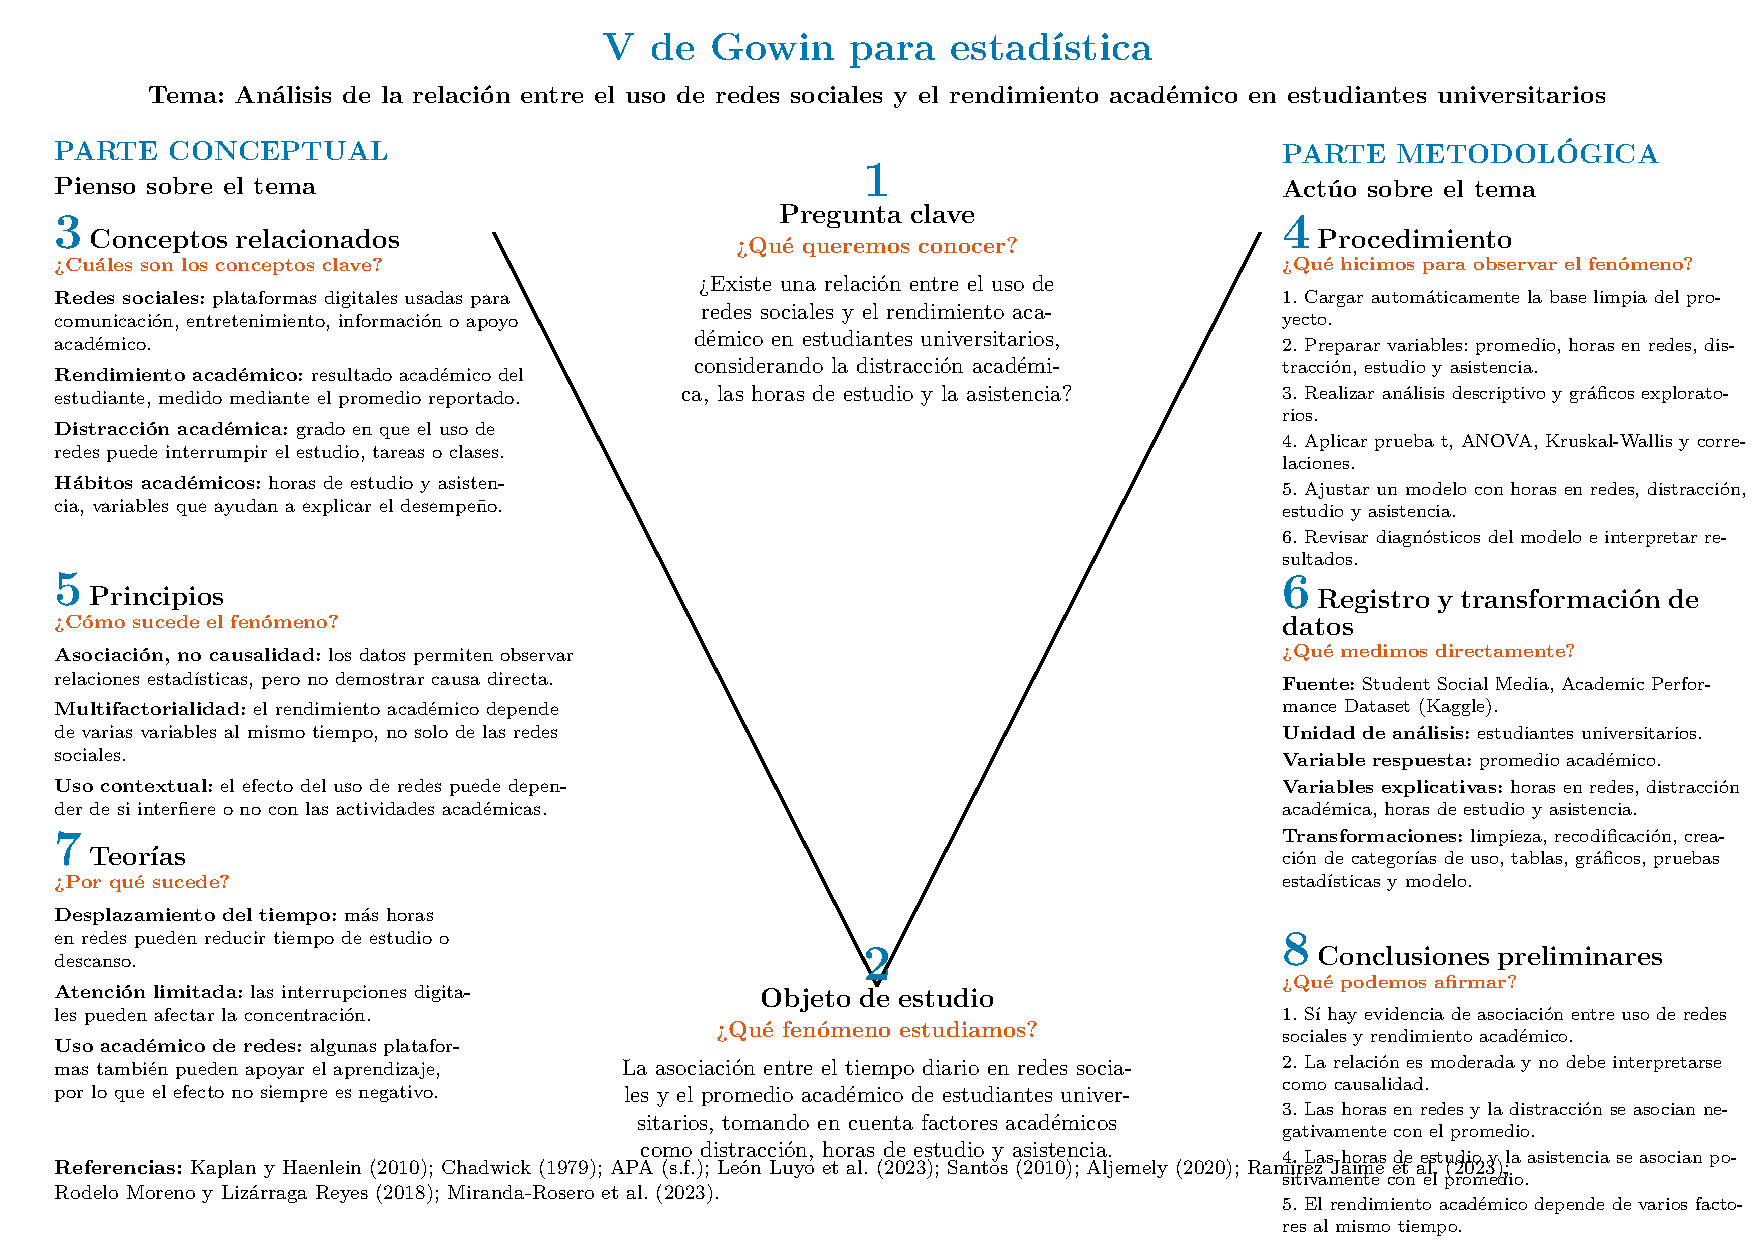
\includepdf[
    pages=1,
    fitpaper=true,
    pagecommand={}
]{uve_actualizada.pdf}

\clearpage

\section{Diario de aprendizaje}

Durante esta etapa aprendimos que observar patrones en gráficos o tablas no es suficiente para concluir que existe una relación entre dos variables. Lo más difícil fue pasar de una interpretación descriptiva a una interpretación estadística, porque tuvimos que decidir qué pruebas usar, cómo justificar el modelo y cómo explicar los resultados sin afirmar causalidad. También vimos que algunas ideas iniciales cambiaron, especialmente la idea de que bastaba con analizar solo las horas de uso de redes sociales. A partir de los resultados obtenidos en la bitácora anterior, comprendimos la importancia de utilizar herramientas estadísticas que permitan evaluar si las diferencias observadas pueden atribuirse realmente a un efecto presente en los datos o si podrían deberse al azar.
\\

También aprendimos que la forma en que se definen y agrupan las variables puede influir en las conclusiones obtenidas. Esto nos llevó a reflexionar sobre las decisiones metodológicas necesarias antes de aplicar cualquier análisis estadístico. El proceso nos ayudó a entender que las decisiones metodológicas, como agrupar variables, revisar supuestos y validar el modelo, son tan importantes como los resultados finales. Ahora sabemos que una investigación no avanza en línea recta, sino que se va ajustando conforme aparecen nuevas preguntas, limitaciones y hallazgos. Finalmente, comprendimos mejor la diferencia entre describir un fenómeno y poner a prueba una hipótesis, entendiendo que la inferencia estadística es una herramienta fundamental para responder preguntas de investigación de manera más rigurosa y fundamentada.


\section{Log de contribuciones}
\section{Registro de uso de IA}

\end{document}
